\documentclass[lang=cn,10pt]{elegantbook}
\usepackage{physics}
\usepackage{unicode-math}
\usepackage{float}
\title{Note for Functional Analysis}

\author{Astolfo}
\version{1.0}

\extrainfo{Too young too simple, sometimes naive.}

\setcounter{tocdepth}{3}

\cover{cover.jpg}

% 本文档命令
\usepackage{array}
\newcommand{\ccr}[1]{\makecell{{\color{#1}\rule{1cm}{1cm}}}}

% 修改标题页的橙色带
% \definecolor{customcolor}{RGB}{32,178,170}
% \colorlet{coverlinecolor}{customcolor}

\begin{document}

\maketitle
\frontmatter


\mainmatter

\chapter*{来自\textit{Astolfo}}
\setcounter{page}{1}
\pagenumbering{roman}
这份讲义是\textit{Astolfo}在大二下旁听\&大三下重修(悲)泛函分析时顺手整理的笔记,\textit{Astolfo}试图通过这种方法让自己好好学习(逃

这份讲义也将作为本人随笔的一部分加入《\textit{Astolfo}的量子化学》系列笔记中,后续其他内容也会陆续加入。

之前忙于学业暂时搁置了该项目,但是最近受迫于升学压力放弃科研加之没什么学业任务后,又重新拾起此书作为摆烂不想科研和学语言时忘记焦虑的办法之一(悲
\begin{flushright}
    \textit{Astolfo} \\ 2023年7月
\end{flushright}
\tableofcontents
\thispagestyle{empty}
\newpage
\setcounter{page}{1}
\pagenumbering{arabic}
\chapter{正式内容前的瞎扯}
回顾常微分方程中的提到的$Picard$定理:

\paragraph*{$Picard$定理} \quad 对初值问题
\[\dv{}{t}x(t)=f(x(t),t) \qquad x(t_0)=x_0 \tag{1-1}\]
如果$f(x(t),t)$在区域$D$上满足$Lipschitz$条件($|f(x_1,t)-f(x_2,t)| \leq L|x_1-x_2|,L>0$对$\forall t \in D$都成立,其实只要在$t_0$的邻域成立即可),
则$\exists \, \varepsilon > 0$,初值问题在$t \in (t_0-\varepsilon,t_0+\varepsilon)$有唯一解$x(t)$。

回顾初等的证法,原初值问题等价于证明积分方程:
\[x(t)=x_0+\int_{t_0}^tf(x(s),s)\dd s \tag{1-2}\]

为证明上述积分方程的存在唯一性,我们可以构造如下函数列$\{x_n(t)\}$(又称$Picard$序列):
\[x_1(t)=x_0+\int_{t_0}^tf(x_0(s),s)\dd s\]
\[x_2(t)=x_0+\int_{t_0}^tf(x_1(s),s)\dd s\]
\[\vdots\]
\[x_{n+1}(t)=x_0+\int_{t_0}^tf(x_n(s),s)\dd s\]
若证得函数列$\{x_n(t)\}$收敛,则其一定会收敛于$x(t)$,即证明初值问题(1)。证明如下:
\begin{equation*}
    \begin{aligned}
        |x_{n+1}-x_n| & =\left|\int_{t_0}^tf(x_n(s),s)\dd s-\int_{t_0}^tf(x_{n-1}(s),s)\dd s\right| \leq \int_{t_0}^t \left| f(x_n(s),s)-f(x_{n-1}(s),s) \right| \dd s \\
        & \leq L\int_{t_0}^t \left| x_n(s)-x_{n-1}(s) \right| \dd s
    \end{aligned}
\end{equation*}
在$t_0$的邻域$(t_0-\varepsilon,t_0+\varepsilon)$上,我们容易得到(取上下确界不改变不等号):
\[|x_{n+1}-x_n| \leq {\mathop {\text{sup}}\limits_{t \in (t_0-\varepsilon,t_0+\varepsilon)}} (L\varepsilon)|x_{n}-x_{n-1}| \leq \cdots \leq {\mathop {\text{sup}}\limits_{t \in (t_0-\varepsilon,t_0+\varepsilon)}} (L\varepsilon)^n|x_1-x_0|\]
由于在$(t_0-\varepsilon,t_0+\varepsilon)$上$f(x(t),t)$满足$Lipschitz$条件,容易得到$f(x(t),t)$在该区间一致连续,故下式有限:
\[|x_1-x_0|=|\int_{t_0}^tf(x_0(s),s)\dd s|<+\infty\]
则:
\[|x_{n+1}-x_n| \leq (L\varepsilon)^nM \ , \ M:={\mathop {\text{sup}}\limits_{t \in (t_0-\varepsilon,t_0+\varepsilon)}} |x_1-x_0| <+\infty\]
进而我们可以得到:
\[|x_m(t)-x_n(t)| \leq M\sum_{i=n}^{m-1}(L\varepsilon)^i\]
取$\varepsilon \leq 1/2L$:
\[|x_m(t)-x_n(t)| \leq M\sum_{i=n}^{m-1}(L\varepsilon)^i \leq M\sum_{i=n}^{m-1}\frac{1}{2^i} < \frac{M}{2^{n-1}}\]
上式两边取极限即证明函数列$\{x_n(t)\}$为一致柯西列,且
\[x_n(t) \rightrightarrows x(t)\]
这时我们回到积分方程
\[x_{n+1}(t)=x_0+\int_{t_0}^tf(x_n(s),s)\dd s\]
对两边取极限,由于$f(x(t),t)$在$(t_0-\varepsilon,t_0+\varepsilon)$上一致连续,积分于极限可交换,(2)得证,进而原初值问题得证。
\[x(t)=\lim_{n \rightarrow +\infty}\left(x_0+\int_{t_0}^tf(x_n(s),s)\dd s\right)=x_0+\int_{t_0}^tf \left (\lim_{n \rightarrow +\infty}x_n(s),s \right )\dd s=x_0+\int_{t_0}^tf(x(s),s)\dd s\]

如果从泛函分析的观点出发,我们可做出如下不严格的说明:

原命题可以写成,取一个连续函数$x(t)$(这里连续意味着可导)满足:
\[x(t)=x_0+\int_{t_0}^tf(x(s),s)\dd s\]

我们记$t_0$的邻域$(t_0-\varepsilon,t_0+\varepsilon)$上全体连续函数的集合为$C(t_0-\varepsilon,t_0+\varepsilon)$,定义一个映射$T$:
\[T \ : \ C(t_0-\varepsilon,t_0+\varepsilon) \rightarrow C(t_0-\varepsilon,t_0+\varepsilon)\]
\[T[x(t)]=x_0+\int_{t_0}^tf(x(s),s)\dd s\]
这时我们的目标就变成了找一个$x(t)$满足$T[x(t)]=x(t)$,即不动点。

我们继续定义$C(t_0-\varepsilon,t_0+\varepsilon)$上的距离(函数空间上的距离):
\[d(x(t),y(t))={\mathop {\text{sup}}\limits_{t \in (t_0-\varepsilon,t_0+\varepsilon)}} |x(t)-y(t)|\]
则:
\[d(T[x(t)],T[y(t)])={\mathop {\text{sup}}\limits_{t \in (t_0-\varepsilon,t_0+\varepsilon)}} \left|\int_{t_0}^tf(x(s),s)\dd s-\int_{t_0}^tf(y(s),s)\dd s \right| \leq L\varepsilon d(x(t),y(t))\]
当取$L\varepsilon < 1$时,我们得到一个压缩映射,由$Banach$不动点定理即证明完毕:
\[d(T[x(t)],T[y(t)]) < d(x(t),y(t))\]

很显然上述只能叫说明,我们并没有定义一个$Banach$不动点定理适用的距离空间出来。不过也足以说明在泛函分析中我们比较感兴趣的两个对象:函数空间和函数空间上的映射。
在上述的说明中,我们通过距离这个几何概念诱导出了这个函数空间的拓扑结构,当然除此之外还有许多其他的拓扑结构也值得讨论,我们在泛函分析中一般默认讨论的函数空间的代数结构是无穷维线性空间。

还有一个值得思考的问题,我们在初等的证明中使用了柯西收敛定理,那么,在函数空间中柯西列一定收敛吗?
答案是否定的,函数空间中只有完备函数空间的柯西列才是收敛的,这个在后续的学习中会涉及。
\chapter{距离空间与拓扑空间}
\begin{introduction}
    \item 距离空间~\ref{def:Metric}
    \item 距离空间的点集~\ref{pointset}
    \item 距离空间的完备性~\ref{complete}
    \item $Baire$定理~\ref{the:Baire}
    \item 压缩映射定理~\ref{zip}
    \item 拓扑空间~\ref{topo}
    \item 距离空间上的紧集~\ref{compact}
    \item $Arzela-Ascoli$定理~\ref{the:AA}
  \end{introduction}
\section{距离空间 $Metric \ Space$}
\subsection{定义及举例}
事实上,我们可以通过定义距离这个几何上的概念很好地定义收敛和连续这两个我们关心的分析上的概念。
例如,在欧氏空间$\mathbb{R}^n$上,我们定义距离:
\[\mathbb{R}^n=\{\overrightarrow{x}=(x_1,x_2,\cdots,x_n)|x_i \in \mathbb{R} \ (i=1,2,\cdots,n)\}\]
\[d(\overrightarrow{x},\overrightarrow{y})=\sqrt{\sum_{i=1}^n\left|x_i-y_i\right|^2}\]
\paragraph*{收敛性} \quad $\overrightarrow{x}_m \rightarrow \overrightarrow{x}$:
\[\overrightarrow{x}_m \rightarrow \overrightarrow{x} \Leftrightarrow d(\overrightarrow{x},\overrightarrow{y}) \rightarrow 0 \Leftrightarrow x_{m,i} \rightarrow x_i \ (i=1,2,\cdots,n)\]
\paragraph*{连续性} \quad 定义函数$f$:
\[f:\mathbb{R}^n \rightarrow \mathbb{R}^m\]
如果$f$满足
\[\overrightarrow{x}_0 \in \mathbb{R}^n\ , \ \forall \varepsilon >0 \ , \ \exists \, \delta >0 \ , \quad s.t. \quad d_{\mathbb{R}^n}(\overrightarrow{x},\overrightarrow{x}_0)<\delta \ , \ d_{\mathbb{R}^m}(f(\overrightarrow{x}),f(\overrightarrow{x}_0))<\varepsilon\]
则称$f$在点$\overrightarrow{x}_0$连续,进而可以推广到处处连续。

从欧氏空间出发,我们可以定义抽象距离空间:
\begin{definition}[抽象距离空间] \label{def:Metric}
    $X$是一个非空集合,$d$是一个定义在$X \times X$上的函数,满足:\\
    1、非负性:$d(x,y) \geq 0$且$d(x,y)=0$当且仅当$x=y$;\\
    2、对称性:$d(x,y)=d(y,x)$;\\
    3、三角不等式:$d(x,y) \leq d(x,z)+d(z,y)$
\end{definition}

下面我们看几个距离空间的例子:
\paragraph*{例1} \quad $C[a,b]$,定义距离
\[d(x(t),y(t))=\mathop{\text{sup}}\limits_{t \in [a,b]}\left|x(t)-y(t)\right|\]
前两个性质显然成立,主要证第三条:

由于由三角不等式恒成立:
\[\left|x(t)-y(t)\right| \leq \left|x(t)-z(t)\right|+\left|z(t)-y(t)\right|\]
两边取上确界即证毕:
\[\mathop{\text{sup}}\limits_{t \in [a,b]}\left|x(t)-y(t)\right| \leq \mathop{\text{sup}}\limits_{t \in [a,b]}\left|x(t)-z(t)\right|+\mathop{\text{sup}}\limits_{t \in [a,b]}\left|z(t)-y(t)\right|\]
\[d(x,y) \leq d(x,z)+d(z,y)\]

\paragraph*{例2} \quad 空间$s=\{x=\{\xi_i\}_{i=1}^{+\infty} \ , \ \xi_i \in \mathbb{R}\}$(规定后续符号对应:$x,t,z \rightarrow \xi,\eta,\psi$),定义距离
\[d(x,y)=\sum_{i=1}^{+\infty}\frac{1}{2^i}\frac{|\xi_i-\eta_i|}{1+|\xi_i-\eta_i|}\]
同样,前两条性质显然,下证第三条:

同样由三角不等式:
\[\left|\xi_i-\eta_i\right| \leq \left|\xi_i-\psi_i\right|+\left|\psi_i-\eta_i\right|\]
\[\sum_{i=1}^{+\infty}\frac{1}{2^i}\frac{|\xi_i-\eta_i|}{1+|\xi_i-\eta_i|} \leq \sum_{i=1}^{+\infty}\frac{1}{2^i}\frac{\left|\xi_i-\psi_i\right|+\left|\psi_i-\eta_i\right|}{1+\left|\xi_i-\psi_i\right|+\left|\psi_i-\eta_i\right|}\]
\[=\sum_{i=1}^{+\infty}\frac{1}{2^i}\frac{\left|\xi_i-\psi_i\right|}{1+\left|\xi_i-\psi_i\right|+\left|\psi_i-\eta_i\right|}+\sum_{i=1}^{+\infty}\frac{1}{2^i}\frac{\left|\psi_i-\eta_i\right|}{1+\left|\xi_i-\psi_i\right|+\left|\psi_i-\eta_i\right|}\]
\[\leq \sum_{i=1}^{+\infty}\frac{1}{2^i}\frac{\left|\xi_i-\psi_i\right|}{1+\left|\xi_i-\psi_i\right|}+\sum_{i=1}^{+\infty}\frac{1}{2^i}\frac{\left|\psi_i-\eta_i\right|}{1+\left|\psi_i-\eta_i\right|}=d(x,z)+d(z,y)\]

\paragraph*{例3} \quad 空间$S(E) \ E \subseteq \mathbb{R}$是$E$上$Lebesgue$可积函数全体,定义距离
\[d(x,y)=\int_E\frac{\left|x(t)-y(t)\right|}{1+\left|x(t)-y(t)\right|}dt\]

证明类似例2。

顺便一说,在这个距离定义下的收敛等价于依测度收敛,下一小节会证明。

\paragraph*{例4} \quad 空间$L^2(E)=\{f\text{在$E$上可测} \ , \ \int_E|f|^2<+\infty\}$上,我们定义距离
\[d(x,y)=\sqrt{\int_E|x(t)-y(t)|^2dt}\]
同样,前两条性质显然,下证第三条:

\[d^2(x,y)=\int_E|x(t)-y(t)|^2dt=\int_E(x^2(t)+y^2(t)-2x(t)y(t))dt\]
\[\leq \int_Ex^2(t)dt+\int_Ey^2(t)dt+2\int_E|x(t)||y(t)|dt \leq \int_Ex^2(t)dt+\int_Ey^2(t)dt+2\sqrt{\int_Ex^2(t)dt}\sqrt{\int_Ey^2(t)dt}\]
\[\leq \left(\sqrt{\int_Ex^2(t)dt}+\sqrt{\int_Ey^2(t)dt}\right)^2\]
此时,如果我们令$x=f-h \ , \ y=g-h$,则上式可改写为
\[d^2(f,g) \leq (d(f,h)+d(g,h))^2\]
原不等式即证。

欧氏空间是距离空间也可类似证明。

上面的几个例子都是函数空间,当然我们也可以来看几个不是函数空间的距离空间的例子。

\paragraph*{例5} \quad 离散空间$X$为任意集合,定义距离
\[d(x,y)=\left \{
\begin{array}{c}
1 \ , \ x \neq y \\ 0 \ , \ x=y
\end{array}   
\right .
\]

\paragraph*{例6} \quad 图($Graph$)

图包含顶点集$V=\{v_1,v_2,\cdots,v_n\}$,边集$E=\{e_{ij}\}$,定义$d(v_i,v_j)$为$v_i$和$v_j$之间最短的路线长度。

\subsection{距离空间的性质}
在上一小节我们介绍了距离空间以及距离的概念,我们可以很自然地引入一般度量意义下的收敛。

\paragraph*{距离空间$(X,d)$上的收敛} \quad 我们称$x_n$收敛于$x$,当其满足
\[\lim_{n \rightarrow \infty}d(x_n,x)=0\]

这里我们回顾一下之前接触过的函数列收敛的种类。

\paragraph*{逐点收敛} \quad $f_n(x) \rightarrow f(x) \ , \ x \in [a,b] \ , \ (n \rightarrow \infty)$
\[\forall x \in [a,b] \ , \ \forall \varepsilon>0 \ , \ \exists \, N(\varepsilon,x)>0 \ , \quad s.t. \quad n \geq N \ , \ |f_n(x)-f(x)|<\varepsilon\]

\paragraph*{一致收敛} \quad $f_n(x) \rightrightarrows f(x) \ , \ (n \rightarrow \infty)$
\[\forall x \in [a,b] \ , \ \forall \varepsilon>0 \ , \ \exists \, N(\varepsilon)>0 \ , \quad s.t. \quad n \geq N \ , \ |f_n(x)-f(x)|<\varepsilon\]

\paragraph*{依测度收敛} \quad $f_n(x) \rightarrow f(x)\textbf{ in measure} \ , \ (n \rightarrow \infty)$
\[\forall \sigma>0 \ , \ \lim_{n \rightarrow \infty}m\{|f_n(x)-f(x)| \geq \sigma\}=0\]

逐点收敛和一致收敛的区别仅在$N$是否与$x$有关,现在我们来考察一下这些收敛跟距离的关系。
我们知道距离这个概念能诱导出收敛,但是收敛并不意味着一定有距离意义。很显然,逐点收敛没有对应的距离意义,因为$N$与$x$有关。

下面我们来看其他两种收敛对应的距离空间上的收敛。

\paragraph*{例1} \quad $X=C[a,b]$
\[d(x(t),y(t))=\mathop {\text{sup}}\limits_{t \in [a,b]}|x(t)-y(t)|\]
\[x_n(t) \rightarrow x(t) \quad (n \rightarrow \infty) \qquad \lim_{n \rightarrow \infty}d(x_n(t),x)=\lim_{n \rightarrow \infty}\mathop {\text{sup}}\limits_{t \in [a,b]}|x_n(t)-x(t)|=0\]
\[\forall \varepsilon>0 \ , \ \exists \, N(\varepsilon)>0 \ , \quad s.t. \quad n \geq N \ , \ \mathop {\text{sup}}\limits_{t \in [a,b]}|x_n(t)-x(t)|<\varepsilon\]
即
\[\forall t \in [a,b] \ , \ \forall \varepsilon>0 \ , \ \exists \, N(\varepsilon)>0 \ , \quad s.t. \quad n \geq N \ , \ |x_n(t)-x(t)|<\varepsilon\]
可见该空间下距离的收敛等价于一致收敛。

\paragraph*{例2} \quad 空间$S(E) \ E \subseteq \mathbb{R}$是$E$上$Lebesgue$可积函数全体
\[d(x,y)=\int_E\frac{\left|x(t)-y(t)\right|}{1+\left|x(t)-y(t)\right|}dt\]
证明:Part 1
\[\lim_{n \rightarrow \infty}d(x_n(t),x(t))=\lim_{n \rightarrow \infty}\int_E\frac{\left|x_n(t)-x(t)\right|}{1+\left|x_n(t)-x(t)\right|}dt=0\]
记$M=\{|x_n(t)-x(t)| \geq \sigma\}\cap E$
\[\int_E\frac{\left|x_n(t)-x(t)\right|}{1+\left|x_n(t)-x(t)\right|}dt \geq \int_M\frac{\left|x_n(t)-x(t)\right|}{1+\left|x_n(t)-x(t)\right|}dt \geq \int_M\frac{\sigma}{1+\sigma}dt=\frac{\sigma}{1+\sigma}m(M)\]
则有
\[0 \leq m(M) \leq \frac{1+\sigma}{\sigma}d(x_n(t),x(t))\rightarrow 0 \quad n \rightarrow \infty\]
于是有
\[f_n(x) \rightarrow f(x)\textbf{ in measure} \ , \ (n \rightarrow \infty)\]
Part 2
\[\int_E\frac{\left|x_n(t)-x(t)\right|}{1+\left|x_n(t)-x(t)\right|}dt=\int_M\frac{\left|x_n(t)-x(t)\right|}{1+\left|x_n(t)-x(t)\right|}dt+\int_{E-M}\frac{\left|x_n(t)-x(t)\right|}{1+\left|x_n(t)-x(t)\right|}dt\]
\[\leq m(M)+\frac{\sigma}{1+\sigma}m(E-M) \leq m(M)+\frac{\sigma}{1+\sigma}m(E)\]
\[\forall \varepsilon>0 \ , \ let \ \sigma=\frac{\varepsilon}{m(E)} \ (assume \ m(E)>1) \ , \ \exists \, N>0 \quad s.t. \quad n \geq N \ , \ m(M)<\varepsilon\]
\[d(x_n(t),x(t)) \leq \varepsilon+\frac{\varepsilon}{1+\sigma}<2\varepsilon\]
\[\lim_{n \rightarrow \infty}d(x_n(t),x(t))=0\]
证毕。

距离空间还有其他的性质如下:

1) 极限存在必定唯一;

2) $x_n \rightarrow x$,则$\{x_{n,i}\} \subset \{x_n\} \quad s.t. \quad x_{n,i} \rightarrow x$ (距离意义下的收敛)

3) $x_n \rightarrow x$,$x_n \rightarrow x$,则有$d(x_n,y_n) \rightarrow d(x,y)$

前两个性质容易得到,我们下证第三条。

由三角不等式
\[d(x_n,y_n) \leq d(x_n,x)+d(x,y)+d(y,y_n) \Leftrightarrow d(x_n,y_n)-d(x,y) \leq d(x_n,x)+d(y_n,y)\]
\[d(x,y) \leq d(x,x_n)+d(x_n,y_n)+d(y_n,y) \Leftrightarrow d(x_n,y_n)-d(x,y) \geq d(x_n,x)+d(y_n,y)\]
\[\Rightarrow \ |d(x_n,y_n)-d(x,y)|=d(x_n,x)+d(y_n,y) \ \rightarrow 0 \ (n \rightarrow \infty)\]
证毕。

我们也可以定义一般度量意义下的连续性。
\paragraph*{距离空间$(X,d)$上的连续} \quad 设$f:(X,d_X) \rightarrow (Y,d_Y)$是距离空间中的映射。我们称$f$在$x_0$处连续,如果其满足
\[\forall x_0 \in X \ , \ \forall \varepsilon>0 \ , \ \exists \, \delta>0 \ , \quad s.t. \quad d_Y(f(x),f(x_0))<\varepsilon \ , \ if \ d_X(x,x_0)<\delta\]

定义了单点连续后我们容易得到如果$f$在任意$x_0 \in X$上都连续我们就称$f$在$X$上连续。

还有一个比较值得探讨的东西是等距映射。
\paragraph*{等距映射} \quad 设$f:(X,d_X) \rightarrow (Y,d_Y)$是距离空间中的映射,若满足
\[\forall x,y \in X \ , \ d_Y(f(x),f(y))=d_X(x,y)\]
则称$f$为等距映射,称$(X,d_X)$与$(Y,d_Y)$等距($isometry$)。

显然,等距映射是连续且单射的,且$x \rightarrow f(x)$是双射。

举个例子,$\mathbb{R}^n \rightarrow \mathbb{R}^n$的等距映射有且仅有合同变换一种。
\[f(\overrightarrow{x})=A\overrightarrow{x}+\overrightarrow{x}_0 \quad A \in O(n)(\text{正交矩阵})\]

\subsection{距离空间的点集} \label{pointset}
这一小节主要是想说明一般度量空间内的如下几个定义:开集、内部、闭集、闭包、稠密性、可分性。这些概念在拓扑学中有更广泛的定义。

首先我们想在度量空间内定义开集,我们首先需要定义开球:
\begin{definition}[开球]
    我们称$B_r(x)=S(x,r)=\{y \in X \ , \ d(x,y)<r\}$为以$x$为球心$r$为半径的开球。
\end{definition}
\begin{definition}[开集]
    设$A \subset X$,如果$A$满足
    \[\forall x \in A \ , \ \exists \, \varepsilon>0 \quad s.t. \quad B_{\varepsilon}(x) \subset A\]
    则称$A$为$X$中的开集。
\end{definition}
进而,我们还能定义内点和内部。
\begin{definition}[内点]
    设$A \subset X$是开集,若
    \[x \in X \ , \ \exists \, \varepsilon>0 \quad s.t. \quad B_{\varepsilon}(x) \subset A\]
    则称$x$是$A$的内点。
\end{definition}
\begin{definition}[内部]
    $A$的全部内点构成的集合称为$A$的内部,记作\AA。
\end{definition}
容易看出$A$是开集$ \ \Leftrightarrow \ A=$\AA。

下面我们来看看开集的基本性质。
\begin{theorem}
    设$(X,d)$是距离空间,则有:\\
    1、$X$,$\varnothing$是开集;\\
    2、任意多个开集的并是开集;\\
    3、有限多个开集的交是开集。
\end{theorem}

前两个性质是显然的,下面我们来看看第三个性质的证明。

假设$G_i \ (i=1,2,\cdots,k)$都是开集。
\[\bigcap_{i=1}^kG_i \neq \varnothing \ \Leftrightarrow \ x \in \bigcap_{i=1}^kG_i \ and \ \exists \, \varepsilon_i >0 \ , \ B_{\varepsilon_i}(x) \subset G_i \quad (i=1,2,\cdots,k)\]
则,我们可以取
\[\varepsilon=\text{min}\{\varepsilon_1,\varepsilon_2,\cdots,\varepsilon_k\} \tag{2-1}\]
使得
\[B_{\varepsilon}(x) \subset B_{\varepsilon_i}(x) \subset G_i \qquad (i=1,2,\cdots,k)\]
即
\[B_{\varepsilon}(x) \subset \bigcap_{i=1}^kG_i\]
证毕。

为什么必须是有限个开集的交?从2-1式我们应该能看出来。
如果是取无限个开集的交,2-1式中的min将无法取到,而应取inf,而取inf的后果将有可能使得$\varepsilon=0$,让后续证明失效。
\begin{definition}[接触点]
    设$A \subset X$是开集,若
    \[x \in X \ , \ \forall \varepsilon>0 \quad s.t. \quad B_{\varepsilon}(x) \cap A \neq \varnothing\]
    则称$x$是$A$的接触点。
\end{definition}

当$x \in A$时,$x$一定是$A$的接触点,$A$的接触点不一定属于$A$。

\begin{definition}[闭包]
    $A$的全部接触点构成的集合称为$A$的闭包,记作$\bar{A}$。
\end{definition}
\begin{definition}[闭集]
    定义1:若$A=\bar{A}$则称$A$为闭集。\\
    定义2:若$A^c$为开集,则$A$为闭集。
\end{definition}

下面我们来看看闭包的性质。
\begin{theorem}
    设$(X,d)$是距离空间,$A,B \subset X$,则有
    \[1)\bar{\varnothing}=\varnothing \, ; \quad 2)A \subset \bar{A} \, ; \quad 3)\bar{\bar{A}}=\bar{A} \, ; \quad 4)\overline{A \cup B}=\bar{A} \cup \bar{B}\]
\end{theorem}

前两点是显然的,我们来证明一下第三第四点。

Proof (2):设
\[x \in \bar{\bar{A}} \ , \ \forall \varepsilon>0 \ , \ B_{\varepsilon}(x) \cap \bar{A} \neq \varnothing\]
\[\Rightarrow \ \exists \, y \in B_{\varepsilon}(x) \cap \bar{A} \ \Rightarrow \ B_{\varepsilon}(y) \cap A \neq \varnothing \ \Rightarrow \ B_{\varepsilon}(y) \subset B_{2\varepsilon}(x) \ \Rightarrow \ B_{2\varepsilon}(x) \cap A \neq \varnothing \ \Rightarrow \ x \in \bar{A}\]

Proof (3):设$x \in \overline{A \cup B}$
\[\forall \varepsilon>0 \ , \ B_{\varepsilon}(x) \cap (A \cup B) \neq \varnothing \ \Rightarrow \ B_{\varepsilon}(x) \cap A \neq \varnothing \ or \ B_{\varepsilon}(x) \cap B \neq \varnothing\]
假设$x \notin \bar{A} \cup \bar{B}$则
\[\exists \, \varepsilon_1,\varepsilon_2>0 \quad s.t. \quad B_{\varepsilon_1}(x) \cap A=\varnothing \ , \ B_{\varepsilon_2}(x) \cap B=\varnothing\]
\[\varepsilon:=\text{min}\{\varepsilon_1,\varepsilon_2\} \ s.t. B_{\varepsilon_1}(x) \cap A=\varnothing \ and \ B_{\varepsilon_2}(x) \cap B=\varnothing\]
矛盾,故$x \in \bar{A} \cup \bar{B}$。

反之,设$x \in \bar{A} \cup \bar{B}$,不妨设$x \in A$,
\[\forall \varepsilon>0 \ , \ B_{\varepsilon}(x) \cap A \neq \varnothing \ \Rightarrow \ \forall \varepsilon>0 \ , \ B_{\varepsilon}(x) \cap (A \cup B) \neq \varnothing \ \Rightarrow  \ x \in \overline{A \cup B}\]
证毕。

下面我们来看闭集的一些性质。
\begin{theorem}
    设$(X,d)$是距离空间,则有:\\
    1、$X$,$\varnothing$是闭集;\\
    2、任意多个闭集的交是闭集;\\
    3、有限多个闭集的并是闭集。
\end{theorem}

这些性质的证明可以通过$De \ Morgan's \ Law$证明类似例2。
\begin{theorem}[$De \ Morgan's \ Law$]
\[\left(\bigcup\limits_{\lambda \in \Lambda}A_{\lambda}\right)^c=\bigcap\limits_{\lambda \in \Lambda}A_{\lambda}^c \qquad \left(\bigcap\limits_{\lambda \in \Lambda}A_{\lambda}\right)^c=\bigcup\limits_{\lambda \in \Lambda}A_{\lambda}^c\]
\end{theorem}

闭集还有如下性质,同时它也是闭集的另一种定义方式:
\begin{theorem}
    设$(X,d)$是距离空间,$A$为闭集,$\{x_n\} \in A$,若$x_n \rightarrow x$,则$x \in A$。
\end{theorem}

下面我们来看稠密性和可分性。

\paragraph*{例1} \quad $\mathbb{R}$中,$\mathbb{Q}$是稠密的($\mathbb{R}$上任意小的区间都有$x \in \mathbb{Q}$);$\mathbb{Q}$是可数的。
\begin{definition}[稠密性]
    若$A \subset X$且$\bar{A}=X$则称$A$在$X$中是稠密的(原本应该是$X \subseteq \bar{A}$,当$X$取全空间的时候只能是$\bar{A}=X$)。
\end{definition}
\begin{definition}[可分性]
    若$X$有可数的稠密子集则称$X$是可分的。
\end{definition}
\paragraph*{例2} \quad $C[a,b]$是可分的

\textbf{Proof:}利用$Weierstrass$定理
\begin{theorem}[$Weierstrass$定理]
    设$f(x)$是$[a,b]$上的连续函数,那么存在一列多项式$\{P_n(x)\}$,使得
    \[P_n(x) \rightrightarrows f(x) \quad (n \rightarrow \infty)\]
\end{theorem}
$\forall P_n(x)$,存在有理多项式列$\{q_{n,i}(x)\}_{i=1}^{\infty}$使得$q_{n,i}(x) \rightrightarrows P_n(x) \ (i \rightarrow \infty)$,则
\[\forall k \in \mathbb{N}_+ \ , \ \exists \, n_k,i_k \ , \ q_{n_k,i_k}(x) \rightrightarrows f(x)\]
再多证明一步即可:
\[d(q_{n_k,i_k}(t),f(t)) \rightarrow 0 \ (n \rightarrow \infty) \ \Leftrightarrow \ q_{n_k,i_k}(x) \rightrightarrows f(x) \tag{*}\]
Proof (*):
\[\forall k \in \mathbb{Z}_+ \ , \ \exists \, n_k>0 \quad s.t. \quad n \geq n_k \ , \ |P_n(t)-f(t)|<\frac{1}{k} \ , \ \forall t \in [a,b]\]
\[\exists \, i_k>0 \ , \quad s.t. \quad i \geq i_k \ , \ |q_{n_k,i_k}(t)-P_{n_k}(t)|<\frac{1}{k} \ , \ \forall t \in [a,b]\]
\[|q_{n_k,i_k}(t)-f(t)| \leq |q_{n_k,i_k}(t)-P_{n_k}(t)|+|P_n(t)-f(t)|<\frac{1}{k}+\frac{1}{k}=\frac{2}{k} \ , \ \forall t \in [a,b]\]
上述是要证的两个条件的共同$\varepsilon-\delta$语言的描述,故(*)证毕。

对上述证明做一下形象化证明,上述的证明实质上是相当于取一个对角线子列$\{a_{i,j}\}$:
\[
\begin{array}{cccccc}
    a_{1,1} & a_{1,2} & a_{1,3} & \cdots & \rightarrow & a_1 \\
    a_{2,1} & a_{2,2} & a_{2,3} & \cdots & \rightarrow & a_2 \\
    \vdots & \vdots & \vdots & \vdots & \rightarrow & \vdots \\
      &   &   &   &   & \downarrow \\
    \vdots & \vdots & \vdots & \vdots & \rightarrow & a_{\infty}
\end{array}    
\]

\paragraph*{例2} \quad $l^{\infty}=\{x|\left\{\xi_i\right\}_{i=1}^{\infty} \ (\xi_i \in \mathbb{R}) \ , \ d(x,0)<\infty\}$,$x$为实数列且$l^{\infty} \in \{\text{所有实数列}\}$,定义$l^{\infty}$上的距离:
\[d(x,y)=\mathop {\text{sup}}\limits_{i=1,2,\cdots}|x_i-y_i| \qquad let \ x=\left\{x_i\right\}_{i=1}^{\infty} \ , \ y=\left\{y_i\right\}_{i=1}^{\infty}\]
是不可分的。

其中有
\[d(x,0)<\infty \Leftrightarrow \mathop {\text{sup}}\limits_{i=1,2,\cdots}|\xi_i|<\infty\]

\textbf{Proof:}易知有:
\[D=\{\left\{\xi_i\right\}_{i=1}^{\infty} \ , \ \xi_i=0 \ or \ 1\} \quad \forall x,y \in D \ , \ d(x,y)=0 \ or \ 1\]
显然,如果我们把$D$中的每一位放到$0.$后面,可以看出就是一个$[0,1]$区间上的二进制表示,故$D$的基数与$\mathbb{R}$相同。
\[card(D)=card([0,1])=card(\mathbb{R})\]

我们利用反证法,假设$l^{\infty}$是可分的,则其可以表示为一个可数稠密子集的闭包
\[l^{\infty}=\bar{A}\]
由于$A$稠密且可数,我们可以知道
\[l^{\infty} \in \bigcup_{a \in A}B_{\frac{1}{3}}(a) \tag{*}\]
(Proof(*): 
\[\forall x \in l^{\infty} \ , \ l^{\infty}=\bar{A} \ \Rightarrow \ x\text{是}A\text{的接触点} \ \Rightarrow \ B_{\frac{1}{4}}(x)\cap A \neq \varnothing\]
\[let \ y \in B_{\frac{1}{4}}(x)\cap A \ \Rightarrow \ x \in B_{\frac{1}{3}}(y) \ \Rightarrow \ x \in \bigcup_{a \in A}B_{\frac{1}{3}}(a)\]
\textbf{Q.E.D.})
\begin{figure}[htbp]
    \center
    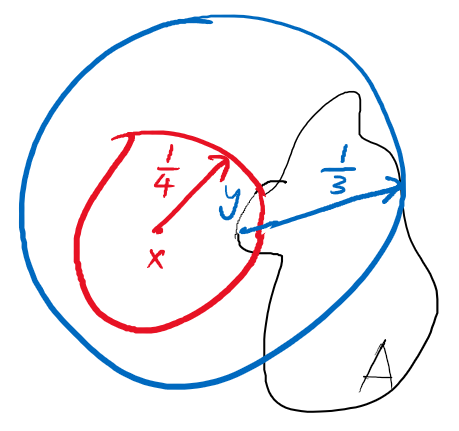
\includegraphics[scale=0.5]{./fig/2.1.3_1.png}
\end{figure}

$A$可数,$D$不可数,且有$D \in l^{\infty} \in \bigcup_{a \in A}B_{\frac{1}{3}}(a)$:
\[\Rightarrow \ \exists \, x \neq y \ , \ x,y \in D \ , \quad s.t. \quad x,y \in \bigcup_{a \in A}B_{\frac{1}{3}}(a) \ (a \in A)\]
\[\Rightarrow \ d(x,y)=1 \leq d(x,a)+d(y,a) \leq \frac{2}{3} \qquad \text{矛盾}\]
故$l^{\infty}$不可分。

\subsection{距离空间的完备性}\label{complete}
\begin{definition}[柯西列]
    设$(X,d)$是距离空间,若$X$中的点列$\{x_n\}_{n=1}^{\infty}$满足:
    \[\{x_n\}_{n=1}^{\infty} \in X \ , \ \forall \varepsilon>0 \ , \ \exists \, N>0 \ , \quad s.t. \quad n,m \geq N \ , \ d(x_n,x_m)<\varepsilon\]
    则称$\{x_n\}_{n=1}^{\infty}$为柯西列。
\end{definition}

\paragraph*{例1} \quad 收敛点列一定是柯西列,柯西列是否一定收敛?

$\mathbb{R}^n$中是,一般距离空间不成立。
\begin{definition}[完备距离空间]
    设$(X,d)$是距离空间。若该距离空间中所有柯西列都收敛,则称距离空间$(X,d)$是完备的。
\end{definition}

\paragraph*{例2} \quad $S=(C[0,1],d_1) \quad d_1(x,y)=\int_0^1|x(t)-y(t)|dt$这个距离空间是不完备的。

找反例,令
\[x_n(t)=\left \{
\begin{array}{ll}
    0 & ,t \in [0,\frac{1}{2}-\frac{1}{n}) \\
    \frac{n}{2}x-\frac{n}{4}+\frac{1}{2} & ,t \in [\frac{1}{2}-\frac{1}{n},\frac{1}{2}+\frac{1}{n}] \\
    1 & ,t \in (\frac{1}{2}+\frac{1}{n},1]
\end{array}
\right .\]
\begin{figure}[htbp]
    \center
    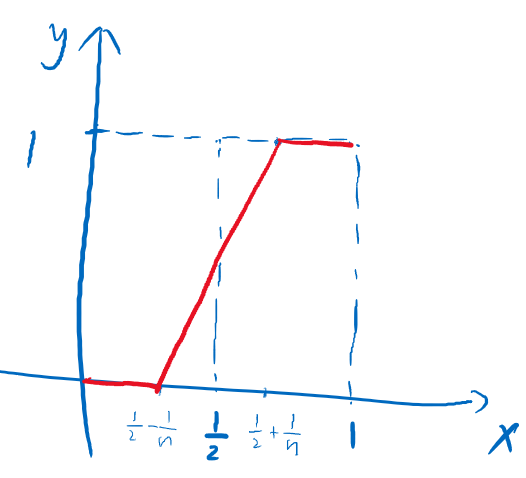
\includegraphics[scale=0.4]{./fig/2.1.4_1.png}
    \caption{$x_n(t)$的图像}
\end{figure}
\[m>n \ , \ d_1(x_n,x_m)=\int_0^1|x_n(t)-x_m(t)|dt \leq \int_{\frac{1}{2}-\frac{1}{n}}^{\frac{1}{2}+\frac{1}{n}}|x_n(t)-x_m(t)|dt \leq \frac{2}{n} \cdot 1=\frac{2}{n}\]
\[\forall \varepsilon>0 \ , \ let \ N>\frac{2}{\varepsilon} \ , \ s.t. m>n \geq N \ d_1(x_m,x_n) \leq \frac{2}{n} < \varepsilon\]
$\{x_n(t)\}$是柯西列。且可以看出$x_n(t)$是逐点收敛(先固定t)于下列函数$x_{\infty}(t)$。
\[x_n(t) \rightarrow x_{\infty}(t)=\left \{
\begin{array}{ll}
    0 & ,t \in [0,\frac{1}{2}) \\
    \frac{1}{2} & ,t=\frac{1}{2} \\
    1 & ,t \in (\frac{1}{2},1]
\end{array}
\right . \qquad (n \rightarrow \infty)\]

采用反证法,假设
\[y \in S \quad s.t. \quad d_1(x_n,y) \rightarrow 0 \ (n \rightarrow \infty) \ \Leftrightarrow \ \int_0^1|x_n(t)-y(t)|dt \rightarrow 0 \ (n \rightarrow \infty)\]
则有
\[d_1(x_{\infty},y) \leq d_1(x_{\infty},x_n)+d_1(x_n,y) \rightarrow 0 \ \Rightarrow \ x_{\infty}(t)=y(t)\]
由$y \in S \ \Rightarrow \ y \in C[0,1]$可得矛盾。

故上述函数列$\{x_n(t)\}$并不在距离空间$(S,d_1)$中收敛。

\paragraph*{例3} \quad $L^2[0,1]$完备
\[L^2[0,1]=\{f\text{在$[0,1]$上可测} \ , \ \int_0^1|f|^2<+\infty\} \quad d(x,y)=\sqrt{\int_0^1(x(t)-y(t))^2dt}\]
\textbf{Proof:}假设$\{x_n(t)\} \in L^2[0,1]$是柯西列,要证其在距离空间收敛$L^2[0,1]$只需证其有收敛子列。
\[\forall k \in \mathbb{Z}_+ \ , \ \exists \, n_k>0 \ , \quad s.t. \quad n,m>n_k \ , \ d(x_n,x_m)<\frac{1}{2^k} \quad (\text{取}n_{k+1}>n_{k})\]
考虑子列$\{x_{n_k}\}_{k=1}^{\infty}$,
\[\int_0^1|x_{n_k}|dt=\int_0^1|x_{n_1}+\sum_{i=2}^k(x_{n_i}-x_{n_{i-1}})|dt \leq \int_0^1|x_{n_1}|dt+\sum_{i=2}^k\int_0^1|x_{n_i}-x_{n_{i-1}}|dt\]
\[\leq \int_0^1|x_{n_1}|dt+\sum_{i=2}^k\left(\int_0^1|x_{n_i}-x_{n_{i-1}}|^2dt\right)^{\frac{1}{2}} \leq \int_0^1|x_{n_1}|dt+\sum_{i=2}^k\frac{1}{2^i}<+\infty\]
由$Fatou$引理:
\[\int_0^1|x_{n_{\infty}}|dt=\int_0^1\varliminf_{k \to \infty}|x_{n_1}+\sum_{i=2}^k(x_{n_i}-x_{n_{i-1}})|dt \leq \varliminf_{k \to \infty}\int_0^1|x_{n_1}+\sum_{i=2}^k(x_{n_i}-x_{n_{i-1}})|dt<+\infty\]
\[\int_0^1\varliminf_{k \to \infty}|x_{n_1}+\sum_{i=2}^k(x_{n_i}-x_{n_{i-1}})|dt<+\infty \ \Rightarrow \ \varliminf_{k \to \infty}|x_{n_1}+\sum_{i=2}^k(x_{n_i}-x_{n_{i-1}})|<+\infty \quad a.e.\]
\[a.e. \ \text{单调有界} \ \Rightarrow \ a.e. \ \text{收敛}\]
\[\varliminf_{k \to \infty}|x_{n_1}+\sum_{i=2}^k(x_{n_i}-x_{n_{i-1}})|=\varliminf_{k \to \infty}|x_{n_k}|<+\infty \quad a.e. \ \text{收敛}\]
极限记为$x_{\infty}(t)$,同样由$Fatou$引理:
\[\int_0^1|x_{\infty}(t)|^2dt \leq \varliminf_{k \to \infty}\int_0^1|x_{n_k}(t)|^2dt<+\infty\]
由控制收敛定理得:
\[\lim_{k \to \infty}\int_0^1|x_{n_k}(t)-x_{\infty}(t)|^2dt=0\]
\textbf{Q.E.D.}
\begin{theorem}[$Fatou$引理]
    设$(S,\Sigma,\mu)$是测度空间,$\{f_n(x)\}$是测度空间上的实值非负可测函数列,则
    \[\int_E\varliminf_{n \to \infty}f_n(x)dx \leq \varliminf_{n \to \infty}\int_Ef_n(x)dx\]
    其中函数极限是在逐点收敛的意义上的极限,函数取值和积分可以是无穷大。
\end{theorem}
\begin{theorem}[控制收敛定理]
    设$(X,\mathscr{F},\mu)$是测度空间,$\{f_n\}$是测度空间上的可测函数列,满足
    \[f_n \xrightarrow{p} f \ or \ f_n \xrightarrow{a.e.} f \ , \ \text{且}\exists \, g \in L^1 \ , \quad s.t. \quad |f_n| \leq g\]
    则
    \[\int f_nd\mu \to \int fd\mu \ (n \to \infty)\]
\end{theorem}

\paragraph*{例4} \quad $L^1[0,1] \quad d_1(x,y)=\int_0^1|x(t)-y(t)|dt \ \{f\text{可测},\int|f|<+\infty\}$完备
\[S=\left(C^1[0,1],d_1\right) \xrightarrow{\text{完备化}} L^1[0,1]\]

\begin{theorem}
    设$(X,d)$是完备距离空间,则\\
    1、所有柯西列收敛; \ 2、闭球套定理; \ 3、$Baire$纲定理
\end{theorem}
\begin{theorem}[闭球套定理]
设$(X,d)$是完备距离空间,假设存在一列闭球
\[\{\bar{B}_{r_i}(x_i)\} \ (i=1,2,\cdots) \ , \quad s.t. \quad \bar{B}_{r_1}(x_1) \supset \bar{B}_{r_2}(x_2) \supset \cdots \quad (r_i \to 0)\]
则
\[\exists \, ! \ x \in \bigcap_{i=1}^{\infty}\bar{B}_{r_i}(x_i)\]
\end{theorem}

\textbf{Proof:}\\
\textbf{Claim 1:$\{x_i\}$是柯西列。}\\
(\textbf{Proof:}
\[r_i \to 0 \ \Leftrightarrow \ \forall \varepsilon>0 \ , \ \exists \, N>0 \ , \quad s.t. \quad i \geq N \ , \ r_i<\varepsilon\]
\[\forall j>i>N \ , \ x_j \in \bar{B}_{r_j}(x_j) \subset \bar{B}_{r_i}(x_i) \ \Rightarrow \ d(x_i,x_j)<r_i<\varepsilon\]
\textbf{Q.E.D.})

下证存在唯一性:\\
(a)存在性:\\
由完备性
\[\exists \, x \in X \ , \quad s.t. \quad d(x_i,x) \rightarrow 0 \ (i \rightarrow \infty)\]
(b)唯一性:\\
假设
\[\exists \, y \in \bigcap_{i=1}^{\infty}\bar{B}_{r_i}(x_i)\]
则
\[d(x,y) \leq d(x,x_i)+d(x_i,y) \rightarrow 0 \ (i \rightarrow \infty)\]
\textbf{Q.E.D.} 

在介绍$Baire$定理之前,我们需要介绍一些定义:
\begin{definition}[疏集]
    设$E \subset X$,若$\bar{E}$不包含任何开球,则称$E$为疏集。
\end{definition}
\paragraph*{例} \quad $\mathbb{Z} \subset \mathbb{R} \ , \ \bar{\mathbb{Z}}=\mathbb{Z}$无开区间,为疏集。
\begin{definition}[第一纲集,第二纲集]
    距离空间$X$可以分成可数个疏集的并,则称$X$为第一纲集,否则称为第二纲集。
\end{definition}
\paragraph*{例} \quad $\mathbb{Q}$是第一纲集,$\mathbb{R}$是第二纲集。
\begin{theorem}[$Baire$定理] \label{the:Baire}
    完备距离空间一定是第二纲集。
\end{theorem}
\textbf{Proof:}\\
反证法:假设完备距离空间$X$是第一纲集,即
\[X=\bigcup_{n=1}^{\infty}E_n \ , \ E_n\text{是疏集}\]
\[\bar{E}_1\text{中无开集} \ \Rightarrow \ \forall x_0 \in X \ , \ r_0>0 \ , \ B_{r_0}(x_0) \nsubseteq \bar{E}_1\]
\begin{figure}[htbp]
    \center
    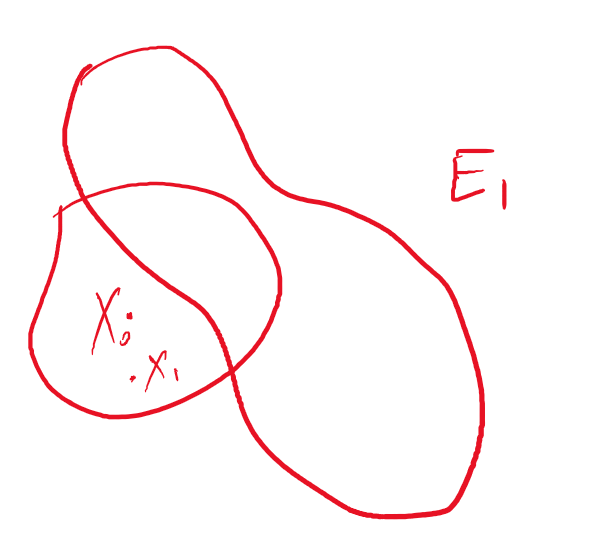
\includegraphics[scale=0.4]{./fig/2.1.4_2.png}
\end{figure}
\[\text{取}x_1 \in B_{r_0}(x_0)-\bar{E}_1=B_{r_0}(x_0)\cap\bar{E}_1^c\text{是个开集,则}\exists \, r_1>0 \ , \quad s.t. \quad B_{2r_1}(x_1) \subset B_{r_0}(x_0)-\bar{E}_1\]
\[\Rightarrow \ \bar{B}_{r_1}(x_1) \subset B_{2r_1}(x_1) \subset B_{r_0}(x_0)-\bar{E}_1\]
\[\text{由于}\bar{E}_2\text{也是疏集} \ , \ B_{r_1}(x_1) \nsubseteq \bar{E}_2\text{则}\exists \, r_2>0 \ , \quad s.t. \quad B_{2r_2}(x_2) \subset B_{r_1}(x_1)-\bar{E}_2\]
\[\Rightarrow \ \bar{B}_{r_2}(x_2) \subset B_{2r_2}(x_2)\cap(\bar{E}_1\cup\bar{E}_2)^c \qquad (\bar{B}_{r_2}(x_2) \subset \bar{B}_{r_1}(x_1) \ and \ \bar{B}_{r_2}(x_2)\cap(\bar{E}_1\cup\bar{E}_2)=\varnothing)\]
由归纳得存在一系列闭球$\{\bar{B}_{r_n}(x_n)\}_{n=1}^{\infty}$
\[s.t. \ \bar{B}_{r_1}(x_1) \supset \bar{B}_{r_2}(x_2) \supset \bar{B}_{r_3}(x_3) \supset \cdots \quad and \quad \bar{B}_{r_n}(x_n)\subset(\bar{E}_1\cup\bar{E}_2\cup\cdots\cup\bar{E}_n)^c=\bigcap_{i=1}^n\bar{E}_i^c\]
\[\Rightarrow \ \bigcap_{i=1}^{\infty}\bar{B}_{r_i}(x_i) \subset \bigcap_{i=1}^{\infty}\bar{E}_i^c=\left(\bigcup_{i=1}^{\infty}\bar{E}_i\right)^c=X^c=\varnothing \quad \text{推出矛盾,故假设不成立}\]
Q.E.D

\subsection{距离空间的完备化与压缩映射} \label{zip}
\paragraph*{例} \quad $S=(C[0,1],d_1) \subset (L^1[0,1],d_1) \ $,$ \ C[0,1]$在$L^1[0,1]$中稠密,称$L^1[0,1]$是$C[0,1]$完备化。\\
\textbf{Proof:}
\[\text{令}x \in L^1[0,1]\text{可积} \ \Leftrightarrow \ \int_0^1|x(t)|dt<+\infty\]
\[\int_0^1|x(t)|dt=\sum_{n=0}^{+\infty} \ \int\limits_{[0,1]\cap\{n \leq |x| \leq n+1\}}|x(t)|dt<+\infty \]
\[ \Rightarrow \ \exists \, N>0 \quad s.t. \quad n \geq N \ , \ \int\limits_{[0,1]\cap\{|x|>N\}}|x(t)|dt<\frac{1}{n}\]
令
\[\tilde{x}(t)=\left \{
\begin{array}{ll}
    x(t) & , x \leq N \\ 0 & , x>N
\end{array}    
\right .\]
由$Lusin$定理,存在连续函数$g_n(t)$,满足
\[m([0,1]/\{\tilde{x}(t)=g_n(t)\})<\frac{1}{nN}\]
\[d_1(g_n(t),x(t)) \leq d_1(g_n(t),\tilde{x}(t))+d_1(\tilde{x}(t),x(t))=\int_0^1|g_n(t)-\tilde{x}(t)|dt+\int_0^1|\tilde{x}(t)-x(t)|dt\]
\[\leq \frac{1}{nN} \cdot N+\int\limits_{[0,1]\cap\{|x(t)|>N\}}|x(t)|dt=\frac{1}{n}+\frac{1}{n}=\frac{2}{n}\]
\[\Rightarrow \ d_1(g_n(t),x(t)) \to 0 \ (n \to \infty)\]
\textbf{Q.E.D.}
\begin{theorem}[$Lusin$定理]
    设$A \in \mathscr{L} \ , \ m(A)<+\infty \ , \ f:A \to \mathbb{R}$是处处有限的$Lebesgue$可测函数,则
    \[\forall \varepsilon>0 \ , \ \exists \, g \in C(A):A\to \mathbb{R} \ , \quad s.t. \quad m(\{g \neq f\}) \leq \varepsilon\]
\end{theorem}
$Lusin$定理实际上表明连续函数和可测函数没太大的差别。

下面我们来介绍一个极其破防的定理以及它更加破防的证明。
\begin{theorem}[完备化定理]
    设$(X,d)$是距离空间,则存在$(\tilde{X},\tilde{d})$是完备距离空间,以及等距映射$F:(X,d) \rightarrow (\tilde{X},\tilde{d})$,且$F(x) \subset (\tilde{X},\tilde{d})$是稠密的。
    称$(\tilde{X},\tilde{d})$是$(X,d)$的完备化。若$(\tilde{Y},\tilde{d}_Y)$是另一个完备化,那么$(\tilde{X},\tilde{d})$与$(\tilde{Y},\tilde{d}_Y)$等距(等距意义下的唯一)。
\end{theorem}
\textbf{Proof:}($\mathbb{Q} \to \mathbb{R}$类似,补全$\mathbb{Q}$中所有柯西列的极限)\\
\textbf{Claim 1 等价类$[\{x_n\}]$}\\
考虑X中所有柯西列的集合,我们称$[\{x_n\}]$和$[\{y_n\}]$等价,如果其满足:
\[\lim_{x \to \infty}d(x_n,y_n)=0 \quad \text{(收敛到同一个点认为是同一类极限)}\]
我们令$\tilde{X}=\{\tilde{x}=[\{x_n\}],\{x_n\}\text{是}X\text{中的柯西列}\} \ $,$ \ [ \quad ]$表示等价类;定义距离
\[\tilde{d}(\tilde{x},\tilde{y})=\lim_{n \to \infty}d(x_n,y_n)\]
下面,我们要证明三件事:1、极限存在;2、$\tilde{d}$的取值与代表元素$x_n,y_n$无关;3、$\tilde{d}$为距离。

1、
\[|d(x_n,y_n)-d(x_m,y_m)| \leq d(x_n,x_m)+d(y_n,y_m)\]
\[\Rightarrow \ \{d(x_n,y_n)\}_{n=1}^{\infty}\text{是}\mathbb{R}\text{中的柯西列} \ \Rightarrow \ \text{收敛} \ \Rightarrow \ \text{该极限存在}\]

2、
\[|d(\tilde{x}_n,\tilde{y}_n)-d(x_n,y_n)| \leq d(\tilde{x}_n,x_n)+d(\tilde{y}_n,y_n)\to 0 \quad (n \to \infty)\]
\[\text{即$\tilde{d}$的收敛性与$[\{x_n\}]$和$[\{x_n\}]$的选取无关}\]

3、
\[\tilde{d}(\tilde{x},\tilde{y})=\lim_{n \to \infty}d(x_n,y_n) \leq \lim_{n \to \infty}d(x_n,z_n)+\lim_{n \to \infty}d(z_n,y_n)=\tilde{d}(\tilde{x},\tilde{z})+\tilde{d}(\tilde{z},\tilde{y})\]
\textbf{Claim 2 $(\tilde{X},\tilde{d})$是完备的}\\
\[\text{设}\{\tilde{x}_n\}\text{是}\tilde{X}\text{中的柯西列,对}\forall \tilde{x} \in \tilde{X}\text{可取代表元}\{x_n\}\text{满足}d(x_n,x_m)\leq \frac{1}{2^k} \ , \ (n,m \geq k)\]
\[(\forall k \ , \ \exists \, n_k>k \ , \quad s.t. \quad n,m \geq n_k \ , \ d(x_n,x_m)<\frac{1}{2^k} \ , \ \text{选取}n_{k+1}>n_k \ , \ \text{则子列}\{x_n\}\text{满足要求})\]
记$\tilde{x}_n=[\{x_{n_i}\}_{i=1}^{\infty}]$,那么我们剩下的事情就是证明任取一个$X$中的柯西列$\{x_n\}$都可以收敛到$\tilde{x}_n$,考虑任取的柯西列的子列$\{x_{n_n}\}$,我们要证明它也是柯西列
\[d(x_{n_n},x_{m_m}) \leq d(x_{n_n},x_{n_m})+d(x_{n_m},x_{m_m}) \leq \frac{1}{2^n}+d(x_{n_m},x_{m_m}) \quad (m>n)\]
其中,对$d(x_{n_m},x_{m_m})$:
\[\forall k \ , \ \exists \, n_k>k \ , \quad s.t. \quad n,m \geq n_k \ , \ \tilde{d}(\tilde{x}_n,\tilde{x}_m)=\lim_{i \to \infty}d(x_{n_i},x_{m_i})<\frac{1}{2^k}\]
\[\Rightarrow \ \exists \, I_k>0 \quad s.t. \quad i \geq I_k \ , \ d(x_{n_i},x_{m_i})<\frac{1}{2^k}\]
\[\Rightarrow \ d(x_{n_m},x_{m_m}) \leq d(x_{n_m},x_{n_{I_k}})+d(x_{n_{I_k}},x_{m_{I_k}})+d(x_{m_{I_k}},x_{m_m}) \leq \frac{1}{2^m}+\frac{1}{2^k}+\frac{1}{2^m} \leq \frac{3}{2^k}\]
\[\Rightarrow \ m,n \geq n_k \ , \ d(x_{n_n},x_{m_m}) \leq \frac{4}{2^k} \ \Rightarrow \ \{x_{n_n}\}\text{为}X\text{中的柯西列}\]
记$\tilde{x}=[\{x_{n_n}\}_{n=1}^{\infty}]$,我们想证明$\tilde{d}(\tilde{x}_n,\tilde{x}) \to 0$
\[\tilde{d}(\tilde{x}_n,\tilde{x})=\lim_{i \to \infty}d(x_{n_i},x_{i_i}) \leq \lim_{i \to \infty}d(x_{n_i},x_{n_n})+\lim_{i \to \infty}d(x_{n_n},x_{i_i}) \leq \frac{1}{2^n}+\frac{1}{2^n}=\frac{2}{2^n}\]
\[\Rightarrow \ \tilde{d}(\tilde{x}_n,\tilde{x}) \to 0 \quad (n \to \infty)\]
\textbf{Claim 3 映射$F:(X,d) \rightarrow (\tilde{X},\tilde{d})$是等距映射,且$F(x) \subset (\tilde{X},\tilde{d})$是稠密的}\\
我们这里定义映射$F$
\[F:(X,d) \to (\tilde{X},\tilde{d}) \quad x \mapsto \tilde{x}=\{x,x,x,\cdots\}\]
$F$是等距映射
\[\tilde{d}(F(x),F(y))=\lim_{n \to \infty}d(\tilde{x},\tilde{y})=d(x,y)\]
记
\[\tilde{x}=[\{x_n\}_{n=1}^{\infty}] \in \tilde{X} \ , \ \tilde{k}_n=\{x_n,x_n,\cdots\} \in F(X)\]
对于$F(x)$的稠密性,我们只需证明,$\forall \tilde{x} \in \tilde{X} \ , \ \exists \, \tilde{k}_n \in F(X) \ , \quad s.t. \quad \tilde{d}(\tilde{k}_n,\tilde{x}) \to 0 \ (n \to \infty)$
\[\tilde{d}(\tilde{k}_n,\tilde{x})=\lim_{i \to \infty}d(k_{n_i},x_i)=\lim_{i \to \infty}d(x_n,x_i) \leq \frac{1}{2^n} \ \Rightarrow \ \tilde{d}(\tilde{k}_n,\tilde{x}) \to 0 \quad (n \to \infty)\]

至此,我们完成了完备化定理存在性部分的证明,我们构造了一个(类)完备距离空间$(\tilde{X},\tilde{d})$,并指出了从原空间$(X,d)$到完备距离空间$(\tilde{X},\tilde{d})$的映射为等距映射,还顺便证明了在等价类意义下,$(X,d)$到$(\tilde{X},\tilde{d})$的映射$F$是一个单射,也即到$(\tilde{X},\tilde{d})$的一个子空间$F(X)$的映射$F$是一个双射。下证唯一性。\\
\textbf{Claim 4 等距意义下的唯一性}\\
设$(\tilde{Y},\tilde{d}_Y)$是$X$的另一个完备化,定义$G:\tilde{Y} \to \tilde{X} \quad y \mapsto [\{x_n\}]$其中$\{x_n\}$是$X$中的一个柯西列,满足
\[\tilde{d}_Y(x_n,y) \to 0 \quad (n \to \infty)\]
因为$\tilde{Y}$,$\tilde{X}$是完备的,故任意给定两个$X$中的柯西列在$\tilde{Y}$,$\tilde{X}$中都能找到对应的像,分别记作$y_1,y_2$和$[\{x_n\}_1],[\{x_n\}_2]$,则
\[\tilde{d}_Y(G(y_1),G(y_2))=\tilde{d}_Y([\{x_n\}_1],[\{x_n\}_2])=\lim_{n \to \infty}\tilde{d}_Y(x_{n_1},x_{n_2})=\tilde{d}_Y(y_1,y_2)\]
即$G$为等距映射(是单射)。\\
\textbf{Q.E.D.}

唯一性证明的部分是想证明所有完备化的距离空间在等距意义下唯一,可以说是想证明等距映射的复合还是等距映射,放到本定理的证明中就是证明$F_x=G \circ F_y$。
\newpage
在完备空间上我们可以定义压缩映射:
\begin{definition}[压缩映射]
    设$(X,d)$是距离空间。若有一映射$T:X \to X$满足
    \[\exists \, \theta \in (0,1) \quad s.t. \quad \forall x,y \in X \ , \ d(T(x),T(y)) \leq \theta d(x,y)\]
    则称$T$为压缩映射。
\end{definition}
\begin{definition}[不动点]
    若$T(x)=x$则称$x$为$T$的不动点。
\end{definition}
\begin{theorem}[压缩映射原理]
    设$(X,d)$是完备距离空间,压缩映射$T:X \to X$,那么$T$有唯一不动点。
\end{theorem}
\textbf{Proof:}\\
\textbf{Claim 1 设$T$是压缩映射(这里不要求完备),$x \in X \ , \ \{T^n(x)\}_{n=0}^{\infty}$是柯西列}\\
(\textbf{Proof:}设$m>n$,
\[d(T^n(x),T^m(x)) \leq \sum_{i=0}^{m-n-1}d(T^{n+i}(x),T^{n+i+1}(x)) \leq \sum_{i=0}^{m-n-1}\theta^{n+i}d(x,T(x))\]
\[=\theta^nd(x,T(x))\sum_{i=0}^{m-n-1}\theta^i=\frac{\theta^n(1-\theta^{m-n})}{1-\theta}d(x,T(x)) < \frac{\theta^n}{1-\theta}d(x,T(x))\]
\[\forall \varepsilon>0 \ , \ \exists \, N>0 \ , \quad s.t. \quad n>N \ , \ \theta^n<\frac{(1-\theta)\varepsilon}{d(x,T(x))} \ \Rightarrow \ \forall m,n \geq N \ , \ d(T^n(x),T^m(x))<\varepsilon\]
)\\
\textbf{存在性}
\[\{T^n(x)\}_{n=0}^{\infty}\text{是柯西列,}X\text{完备} \ \Rightarrow \ \exists \, x_{\infty} \in X \ , \ d(T^n(x),x_{\infty}) \to 0\]
\[T^n(x)=T\left(T^{n-1}(x)\right) \ (n \to \infty) \ \Rightarrow \ x_{\infty}=T(x_{\infty}) \quad (\text{需要}T\text{连续,容易证明})\]
\[\text{上一小步完整证明:}x_{\infty}=\lim_{n \to \infty}T^n(x)=\lim_{n \to \infty}T(T^{n-1}(x))=T(\lim_{n \to \infty}T^{n-1}(x))=T(x_{\infty})\]
\textbf{唯一性}
\[\text{设}T(x)=x \ , \ T(y)=y\]
\[d(x,y)=d(T(x),T(y)) \leq \theta d(x,y) \ \Rightarrow \ d(x,y)=0\]
\begin{proposition}[推广的压缩映射原理]
    设$(X,d)$是完备距离空间,$T:X \to X$满足
    \[\exists \, n_0 \in \mathbb{Z} \ , \ \theta \in (0,1) \ , \quad s.t. \quad d(T^{n_0}(x),T^{n_0}(y))<\theta d(x,y) \ , \ \forall x,y \in X\]
    则$T$有唯一不动点。(不要求$T$是压缩映射,但$T$复合$n_0$次后是压缩映射)
\end{proposition}
\textbf{Proof:}
\[\exists \, ! \, x \in X \quad s.t. \quad T^{n_0}(x)=x \ \Rightarrow \ T \circ T^{n_0}(x)=T(x) \ \Leftrightarrow \ T^{n_0}(T(x))=T(x) \Rightarrow \ T(x)\text{是}T^{n_0}\text{的不动点}\]
\[\text{由唯一性可得}T(x)=x\]

\textbf{Q.E.D.}

下面我们来看几个压缩映射原理应用的例子(证明方程解的唯一性)。
\paragraph*{例1}
\[\vec{\xi}-A\vec{\xi}=\vec{b} \ (\vec{\xi},\vec{b}\in\mathbb{R}^n \ , \ A=[A]_{n \times n}) \ , \ \text{设}A=\{a_{ij}\}\text{且满足} \ 0<\sum_{i=1}^n\sum_{j=1}^na_{ij}^2<1\]
证明:方程存在唯一解。\\
\[X=\mathbb{R}^n\text{ (完备)} \quad T(\vec{\xi})=A\vec{\xi}+\vec{b} \quad \vec{\xi},\vec{\eta} \in X\]
\[d(\vec{\xi},\vec{\eta})=|T(\vec{\xi})-T(\vec{\eta})|=|A(\vec{\xi}-\vec{\eta})|=\sqrt{\sum_{i=1}^n\left(\sum_{j=1}^na_{ij}(\xi_j-\eta_j)\right)^2}\]
\[\leq \sqrt{\sum_{i=1}^n\left(\sum_{j=1}^na_{ij}\right)^2\left(\sum_{k=1}^n(\xi_k-\eta_k)\right)^2}=\sqrt{\sum_{i=1}^n\sum_{j=1}^na_{ij}^2}|\vec{\xi}-\vec{\eta}|=\theta|\vec{\xi}-\vec{\eta}| \quad (\theta \in (0,1))\]
后续证明略
\paragraph*{例2} \quad $Fredholm$积分方程
\[x(t)=\psi(t)+\lambda\int_a^bK(t,s)x(s)ds \ , \ K(t,s) \in C[a,b] \times [a,b] \ , \ \psi(t) \in C[a,b]\]
证明:当$\lambda$足够小的时候方程有唯一解。\\
\[X=C[a,b]\text{ (完备)} \quad d(x,y)=\mathop {\text{sup}}\limits_{t \in [a,b]}|x(t)-y(t)| \ (x(t),y(t) \in X)\]
\[\text{定义}T:C[a,b] \to C[a,b] \quad T(x(t))=\psi(t)+\lambda\int_a^bK(t,s)x(s)ds\]
\[d(T(x(t)),T(y(t)))=\mathop {\text{sup}}\limits_{t \in [a,b]}|T(x(t))-T(y(t))|=\lambda\mathop {\text{sup}}\limits_{t \in [a,b]}\left|\int_a^bK(t,s)(x(s)-y(s))ds\right|\]
$K(t,s)$在闭区域上连续,可得$K(t,s)$有界。
\[d(T(x(t)),T(y(t))) \leq \lambda\mathop {\text{sup}}\limits_{t \in [a,b]}\int_a^b|K(t,s)||x(s)-y(s)|ds \leq \lambda\mathop {\text{sup}}\limits_{t \in [a,b]}|K(t,s)|d(x,y)(b-a)\]
\[\text{当}\lambda\mathop {\text{sup}}\limits_{t \in [a,b]}|K(t,s)|(b-a)<1\text{时,$T$为压缩映射} \ \Rightarrow \ d(T(x(t)),T(y(t))) \leq \theta d(x,y)\]
后续证明略
\paragraph*{例3} \quad $Volterra$积分方程
\[x(t)=\psi(t)+\lambda\int_a^tK(t,s)x(s)ds \ , \ K(t,s) \in C(([a,b] \times [a,b])\cap\{s<=t\}) \ , \ \psi(t) \in C[a,b]\]
\begin{figure}[htbp]
    \center
    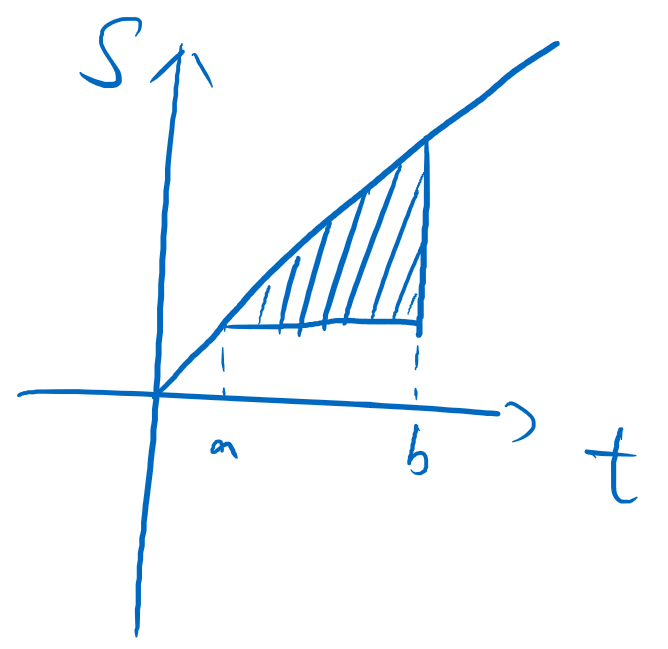
\includegraphics[scale=0.25]{./fig/2.1.5-1.png}
\end{figure}
证明:方程有唯一解。\\
\[T:C[a,b] \to C[a,b] \quad T(x(t))=\psi(t)+\lambda\int_a^tK(t,s)x(s)ds\]
\[d(T(x(t)),T(y(t)))=\lambda\mathop {\text{sup}}\limits_{t \in [a,b]}\left|\int_a^tK(t,s)(x(s)-y(s))ds\right| \leq \lambda\mathop {\text{sup}}\limits_{t \in [a,b]}\left|K(t,s)\right|d(x,y)(t-a)\]
\[d(T^2(x(t)),T^2(y(t)))=\lambda\mathop {\text{sup}}\limits_{t \in [a,b]}\left|\int_a^tK(t,s)\lambda\left|\int_a^tK(t,s)(x(s)-y(s))ds\right|ds\right|\]
\[\leq \lambda^2\left(\mathop {\text{sup}}\limits_{t \in [a,b]}\left|K(t,s)\right|\right)^2d(x,y)\mathop {\text{sup}}\limits_{t \in [a,b]}\left|\int_a^t\int_a^sd\tilde{s}ds\right|\]
\[=\lambda^2\left(\mathop {\text{sup}}\limits_{t \in [a,b]}\left|K(t,s)\right|\right)^2d(x,y)\mathop {\text{sup}}\limits_{t \in [a,b]}\left(\frac{(t-a)^2}{2}\right)=\lambda^2\left(\mathop {\text{sup}}\limits_{t \in [a,b]}\left|K(t,s)\right|\right)^2d(x,y) \cdot \frac{(b-a)^2}{2}\]
易得
\[d(T^n(x(t)),T^n(y(t))) \leq \left(\mathop {\text{sup}}\limits_{t \in [a,b]}\left|K(t,s)\right|\right)^n \cdot \frac{\lambda^n(b-a)^n}{n!}d(x,y):=\frac{\lambda^nM^n(b-a)^n}{n!}d(x,y)\]
\[\lim_{n \to \infty}\frac{\lambda^nM^n(b-a)^n}{n!}=0 \ \Rightarrow \ \exists \, n_0 \ , \quad s.t. \quad \theta=\frac{\lambda^{n_0}M^{n_0}(b-a)^{n_0}}{{n_0}!}<1 \ \Rightarrow \ T^{n_0}\text{是压缩映射}\]
后续证明略
\paragraph*{例extra} \quad $C[a,b]$的完备性 \\
一般来说$C[a,b]$默认的距离应该是
\[d(x,y)=\mathop {\text{sup}}\limits_{t \in [a,b]}|x(t)-y(t)|\]
我们设$\{x_n(t)\}_{i=1}^{\infty}$是柯西列:
\[\forall t \in [a,b] \ , \ \forall \varepsilon>0 \ , \ \exists \, N>0 \ , \ s.t. \forall m,n \geq N \ , \ d(x_n(t),x_m(t))<\varepsilon\]
\[\Leftrightarrow \ \forall t \in [a,b] \ , \ \forall \varepsilon>0 \ , \ \exists \, N>0 \ , \ s.t. \forall m,n \geq N \ , \ |x_n(t)-x_m(t)|<\varepsilon \tag{*}\]
即$x_n(t) \xrightarrow{\text{逐点}} x(t)$
\[\text{令(*)式中 }m \to \infty \ , \ \forall \varepsilon>0 \ , \ \exists \, N>0 \ , \quad s.t. \quad \forall n \geq N \ , \ |x_n(t)-x(t)|<\varepsilon\]
即$x_n(t) \rightrightarrows x(t)$(连续函数一致收敛到连续函数上)
\paragraph*{例4}
\[\left\{
\begin{array}{c}
    \frac{\partial}{\partial t}f(x,t)=\Delta f(x,t)+G(f(x,y)) \quad x \in \mathbb{R}^n \ , \ t \in [0,+\infty) \\
    f(x,0)=\phi(x)
\end{array}
\right.\]
\[\text{设}\phi(x),G(s)\text{有界连续},G(s)\text{在}\mathbb{R}\text{上} 𝐿𝑖𝑝𝑠𝑐ℎ𝑖𝑡𝑧 \text{连续,即}|G(a)-G(b)| \leq L|a,b| \ \forall a,b \in \mathbb{R}\]
令
\[f_0(x,t)=\int_{\mathbb{R}^n}H(x,y,t)\phi(y)dy\]
热方程的解$=$热核$*$(卷)上初始条件。热核:
\[H(x,y,t)=\frac{1}{(4 \pi t)^{\frac{n}{2}}}e^{-\frac{|x-y|^2}{4t}}\]
满足
\[\frac{\partial}{\partial t}f_0=\Delta f_0 \quad \eval{f_0(x,t)}_{t=0}=\phi(x)\]
令
\[T(f(x,t))=f_0(x,t)+\int_0^t\int_{\mathbb{R}^n}H(x,y,t-s)G(f(y,s))dyds\]
后面老师没讲我不会了(寄)。

\section{拓扑空间$Topological \ Space$} \label{topo}
\subsection{真·拓扑空间不完全简介}
在距离空间中,我们是通过距离这个概念引入了开球、开集等集合概念与距离空间中的收敛这个概念,由开球和开集进而导出连续性、紧性;由收敛性我们给出完备性的概念。
\begin{figure}[htbp]
    \center
    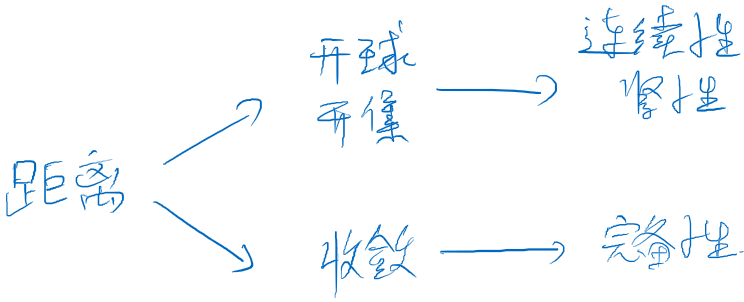
\includegraphics[scale=0.4]{./fig/2.2.1.png}
\end{figure}
但实际上,我们知道(可能不知道)连续性、紧性不一定需要由距离这个概念诱导得到,定义他们只需要开集。

以及在收敛中,我们也发现了弱收敛、逐点收敛并不具有距离概念。

显然距离空间并不是一个足够广泛的空间可以支撑得起这些概念,因此,我们需要考虑一个更广泛的空间,这里我们讲简要介绍拓扑空间。
\begin{definition}[拓扑]
    设$X \neq \varnothing$,记$P(X)=\{X\text{的所有子集}\}$,设$\tau \in P(X)$满足:\\
    \textbf{1.} $\varnothing,X \in \tau$; \qquad \textbf{2.} $\tau$中任意个集合的并属于$\tau$; \qquad \textbf{3.} $\tau$中有限个集合的交属于$\tau$。\\
    则称$\tau$是$X$上的拓扑,$\tau$中的集合称为开集。(拓扑就是指定集合上的哪些子集是开集)
\end{definition}
\paragraph*{例1} $(X,d)$是距离空间,$\tau_d=\{x\text{中的开集}\}$
\paragraph*{例2} $X=\{0,1\}$,令
\[\tau_1=\{\varnothing,X\}\text{(平凡拓扑)} \quad \tau_2=\{\varnothing,\{0\},X\}\text{(是个拓扑)}\]
\[\tau_3=\{\varnothing,\{0\},\{1\},X\}\text{(离散拓扑,由$X$的所有子集组成的拓扑,包含$X$的所有单点集)}\]

若在$X$上,$\tau_1 \subset \tau_2$,则称$\tau_2$强于$\tau_1$。
\begin{definition}[闭集]
    若$A^c \in \tau$,则称$A$是闭集。($A$是闭集$\ \Leftrightarrow \ A=\bar{A}$)
\end{definition}
\begin{definition}[邻域]
    设$x \in X \ , \ U_x \subset \tau \ , \ x \in U_x$,则称$U_x$是$x$的一个邻域(包含$x$的开集)
\end{definition}
\begin{definition}[连续]
    定义$f:X \to Y$是拓扑空间到拓扑空间的映射,设$x_0 \in X$,若对任意$f(x_0)$的邻域$V_{f(x_0)}$都存在$X$中$x_0$的邻域$U_{x_0}$使得$f(U_{x_0}) \subset V_{f(x_0)}$,则$f$称在$x_0$处连续。
\end{definition}
\begin{theorem}
    若$X,Y$是拓扑空间,$f:X \to Y$是连续映射当且仅当开集的原像是开集。
\end{theorem}
这里我们规定符号$f^{-1}$仅表示原像
\[f:X \to Y \ (A \subseteq Y) \quad f^{-1}(A)=\{x \in X \ , \ f(x) \in A\}\]
最后给个奇怪的例子作为这一小节的总结,在下一小节虽然我们也将介绍一些拓扑空间中可以定义的概念,但我们更愿意将他放到距离空间的背景下来考量,因为这门课是泛函分析(乐)。
\paragraph*{奇怪的例子} 定义如下拓扑

$X=\{0,1\} \quad \tau_D=\{\varnothing,\{0\},\{1\},X\}$单点集在$\mathbb{R}^n$和距离空间中是闭集,但这里是开集。

\subsection{紧集}
在介绍距离空间上的紧性之前,我们需要介绍一下四种分离公理并指认距离空间所属的公理。
\begin{proposition}[分离公理]
    $T_1$公理:$\forall x \neq y \ , \ \exists \, U_x,U_y \ , \quad s.t. \quad x \in U_x \ , \ y \notin U_x \ ; \ y \in U_y \ , \ x \notin U_y$\\
    $T_2$公理:$\forall x \neq y \ , \ \exists \, U_x \cap U_y=\varnothing \ , \quad s.t. \quad x \in U_x \ , \ y \notin U_x \ ; \ y \in U_y \ , \ x \notin U_y$\\
    $T_3$公理:$\forall$ 闭集$A \cap x=\varnothing \ , \ \exists \, U_x \cap U_A=\varnothing \ , \quad s.t. \quad x \in U_x \ , \ A \notin U_x \ ; \ A \in U_A \ , \ x \notin U_A$\\
    $T_4$公理:$\forall$ 闭集$A \cap B=\varnothing \ , \ \exists \, U_A \cap U_B=\varnothing \ , \quad s.t. \quad A \in U_A \ , \ B \notin U_A \ ; \ B \in U_B \ , \ B \notin U_A$
\end{proposition}
很显然,这四个公理的限制逐级加强,下面我们可以来看看这几个公理的形象化描述:
\begin{figure}[htbp]
    \center
    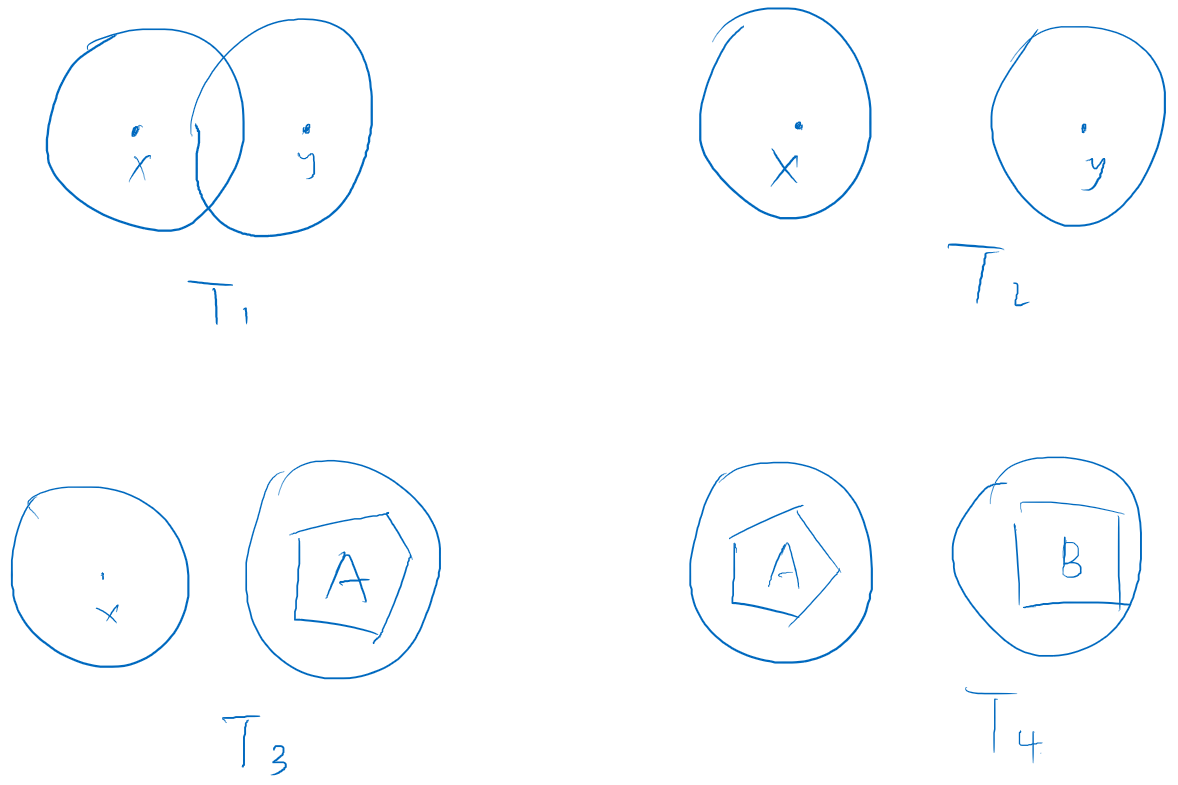
\includegraphics[scale=0.4]{./fig/2.2.2.png}
\end{figure}
对应$T_2$公理,我们又将其称为$Hausdorff$性质,距离空间是满足$T_4$公理的,对于这件事我们可以来证明一下。
\begin{theorem}
    距离空间满足$T_4$公理。
\end{theorem}
Proof(反证法):先预设一些对象:
\[\bar{A}=A \ , \ \bar{B}=B \ , \ A \cap B=\varnothing \ , \ f_A(x):=\mathop {\text{inf}}\limits_{y \in A}d(x,y) \ , \ f_B(x):=\mathop {\text{inf}}\limits_{y \in B}d(x,y)\]
\textbf{Claim} \quad $f_A(x)>0 \ \Rightarrow \ x \notin A$\\
(\textbf{Proof:}反证法

若$f_A(x)=0 \ \Rightarrow \ \exists \, \{y_n\} \subset A \quad s.t. \quad d(x,y_n) \to 0 \ \Rightarrow \ x$是$A$的接触点$ \ \Rightarrow \ x \in \bar{A}=A$\\
矛盾)\\
记
\[U_B=\bigcup_{x \in B}B_{\frac{1}{2}f_A(x)}(x) \ , \ B \subset U_B \qquad U_A=\bigcup_{x \in A}B_{\frac{1}{2}f_B(x)}(x) \ , \ A \subset U_A \quad \text{都是开集}\]
假设
\[\exists \, z \in U_A \cap U_B \ \Rightarrow \ \exists \, x \in A \quad s.t. \quad z \in B_{\frac{1}{2}f_B(x)}(x) \ , \ \exists \, y \in B \quad s.t. \quad z \in B_{\frac{1}{2}f_A(y)}(y)\]
\[\Rightarrow \ d(x,z)<\frac{1}{2}f_B(x) \ , \ d(z,y)<\frac{1}{2}f_A(y)\]
\[d(x,y) \leq d(x,z)+d(z,y)<\frac{1}{2}f_B(x)+\frac{1}{2}f_A(y)<\frac{1}{2}d(x,y)+\frac{1}{2}d(x,y)=d(x,y)\]
矛盾。
\begin{definition}[子集拓扑]
    $(X,\tau)$为拓扑空间,$A \subset X$,令$\tau_A=\{U \cap A \ , \ U \in \tau\}$,则称$\tau_A$为$X$上的子集拓扑(诱导拓扑)。
\end{definition}
下面,我们将要开始引入我们我们这小节的主要内容,刻画距离空间的紧性,接着上面的内容,我们先看看拓扑空间下紧性的定义。
\begin{definition}[紧(致)性]
    $(X,\tau)$为拓扑空间,若$X$的任意开覆盖都有有限子覆盖,则称$X$是紧(致)的。
    \[X \subset \bigcup_{\lambda \in \Lambda}A_{\lambda} \ \text{$A_{\lambda}$是开集} \ \Rightarrow \ X \subset \bigcup_{i=1}^kA_{\lambda_i}\]
\end{definition}
\paragraph*{例} $\mathbb{R}^n$上的闭区间(有界闭集)是紧的。
\begin{definition}[紧集]
    $(X,\tau)$为拓扑空间,$A \subset (X,\tau)$,若$(A,\tau_A)$是紧的,则称$A$是$X$中的紧集。
\end{definition}
下面我们将讨论拓扑空间下闭集和紧集的关系,我们知道欧氏空间中紧集就是有界闭集,那么这个性质在一般的拓扑空间中还成立吗?
\begin{theorem}
    紧空间的闭子集一定是紧集。
\end{theorem}
\textbf{Proof:}设$X$是一紧空间(或者拓扑空间中的紧子集),$A \subset X$,设
\[A \subset \bigcup_{\lambda \in \Lambda}U_{\lambda} \ \Rightarrow \ X \subset \left(\bigcup_{\lambda \in \Lambda}U_{\lambda}\right) \cup A^c\]
因为$X$是紧的,有
\[\exists \, \lambda_1,\lambda_2,\cdots,\lambda_k>0 \quad s.t. \quad X \subset \left(\bigcup_{i=1}^kU_{\lambda_i}\right) \cup A^c\]
\[A \subset X \subset \left(\bigcup_{i=1}^kU_{\lambda_i}\right) \cup A^c\]
故$A$是紧的。\\
\textbf{Q.E.D.}
\begin{theorem}
    $T_2$空间的紧子集是闭集。
\end{theorem}
\textbf{Proof:}设$X$是$T_2$空间,$A \subset X$,需证明$A^c$为开集,即需证$\forall x \in A^c \ , \ \exists \, U_x \subset A^c$。

设$y \in A \ , \ x \in A^c$,由$T_2$公理,存在$x$的开邻域$U_{x,y}$,$y$的开邻域$V_{x,y}$($U_{x,y},V_{x,y}$选取与$x,y$都有关)满足$U_{x,y} \cap V_{x,y}=\varnothing$
\[\Rightarrow \ A \subset \bigcup_{y \in A}V_{x,y} \ , \ \text{由紧性} \ , \ \exists \, y_1,y_2,\cdots,y_k \in A \quad s.t. \quad A \subset \bigcup_{i=1}^kV_{x,y_i}\]
\[\text{令}U_x=\bigcup_{i=1}^kU_{x,y_i} \ \Rightarrow \ U_x \cap \bigcup_{i=1}^kV_{x,y_i}=\varnothing \ \Rightarrow \ U_x \cap A=\varnothing \ \text{即} \ U_x \cap A^c\]
\textbf{Q.E.D.}

可以看到,在一般拓扑空间下紧和闭是两个等同的概念,紧比闭更强一点。下面我们来看一个紧的性质结束这一小节。
\begin{theorem}
    紧空间(子集)在连续映射下的像也是紧的。
\end{theorem}
\textbf{Proof:}
\begin{figure}[htbp]
    \center
    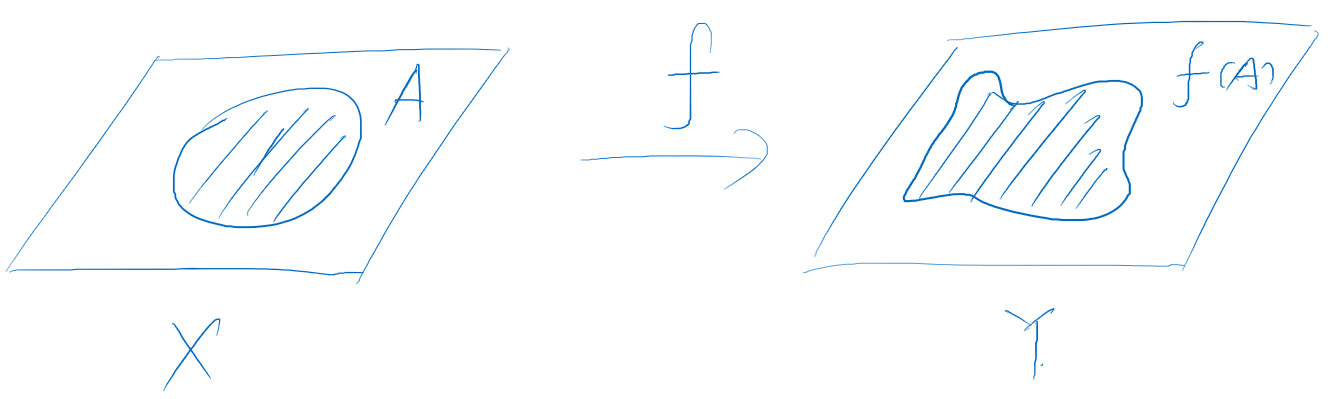
\includegraphics[scale=0.2]{./fig/2.2.2-1.png}
\end{figure}
\[\text{设}A \subset X\text{是紧的,}f(A) \subset \bigcup_\alpha G_\alpha \ , \ \{G_{\alpha}\}\text{为}Y\text{中的一族开集}\]
\[\text{由$f$为连续映射可得}f^{-1}(G_{\alpha})\text{是开集且}A \subset \bigcup_{\alpha}f^{-1}(G_{\alpha})\]
\[\text{由$A$紧可得} \exists \, \alpha_1,\alpha_2,\cdots,\alpha_k \quad s.t. \quad A \subset \bigcup_{i=1}^kf^{-1}(G_{\alpha_1}) \ , \ f(A) \subset \bigcup_{i=1}^kG_{\alpha_i}\]

\textbf{Q.E.D.}

\subsection{刻画距离空间上的紧集} \label{compact}
下面我们来看距离空间中的紧集是如何定义的。
\begin{definition}[距离空间中的紧集]
    $(X,d)$为距离空间,$A \subset X$,
    \[A \subset \bigcup_{\lambda \in \Lambda}B_{r_{\lambda}}(x_{\lambda})\text{是$A$的任一开球覆盖必有一有限子覆盖}\bigcup_{i=1}^kB_{r_{\lambda_i}}(x_{\lambda_i})\]
    则称$A$是$X$中的紧集。
\end{definition}
顺便再额外看一下有界性的定义。
\begin{definition}[距离空间中的有界性]
    $(X,d)$为距离空间,$A \subset X$,
    \[\exists \, R>0 \ , \ x \in X \ , \quad s.t. \quad A \subset B_R(x)\]
    则称$A$有界。
\end{definition}
\paragraph*{例1} $\mathbb{R}^n$上的紧集是有界闭集,但在一般距离空间中不再成立。

\paragraph*{例2} $l^2$空间是完备的,其上的闭球$\bar{B}_1(0)$不是紧集。
\[l^2=\left\{\{x_n\}_{n=1}^{\infty} \ , \ x_n \in \mathbb{R} \ , \ \sum_{n=1}^{\infty}x_n^2<\infty\right\} \quad d(x,y)=\sqrt{\sum_{n=1}^{\infty}(x_n-y_n)^2}\]
\textbf{Proof:}令$x_n=\{0,0,\cdots,1,0,\cdots\}$(第$n$个为$1$) \quad $x_n \in \bar{B}_1(0) \ (d(x_n,0)=\sqrt{1^2}=1)$
\[\forall n \neq m \ , \ d(x_n,x_m)=\sqrt{1^2+1^2}=\sqrt{2} \ \text{当$m,n$足够大的时候并不趋于0} \ \Rightarrow \ \bar{B}_1(0)\text{不是列紧的}\]
在后续的介绍中,我们会证明,度量空间中列紧的闭集就是紧集,所以这里我们就能看出$\bar{B}_1(0)$不是紧集。当然我们需要解释一下什么是列紧。
\begin{definition}[(相对)列紧性]
    若集合$A$中的任意点列都有收敛子列,则称$A$是列紧的,不要求极限也在$A$中(当$A$为闭时,则极限必然在$A$中,但列紧性要求极限在集合中)。
\end{definition}
在上述例子中我们可以看出列紧是比紧更弱一点的条件。下面我们给出一般距离空间和完备距离空间中紧集的完整刻画,并证明他们。
\begin{theorem}
    距离空间中的子集是紧集当且仅当它是列紧的闭集。
\end{theorem}
\textbf{Proof:}(紧$ \ \Rightarrow \ $列紧闭)
\[A \text{是列紧的闭集} \ \Leftrightarrow \ \forall\{y_n\} \subset A\text{都有收敛子列}y_{n_k} \to y \in A\]

反证法:设$\{y_n\} \subset A$,它的任意子列不收敛于$A$中的点。
\[\forall x \in A \ , \ \exists \, r_x>0 \ , \ B_{r_x}(x) \cap \{y_n\}=\{y_{n_1},y_{n_2},\cdots,y_{n_k}\} \ (k<\infty) \ , \ A \subset \bigcup_{x\in A}B_{r_x}(x)\]
由$A$的紧性:
\[\exists \, x_1,x_2,\cdots,x_k \in A \ , \quad s.t. \quad A \subset \bigcup_{i=1}^kB_{r_{x_i}}(x_i) \ \Rightarrow \ A \cap \{y_n\}=\{y_{n_1},y_{n_2},\cdots,y_{n_j}\} \ (j<\infty)\]
推出矛盾。\\
\textbf{Q.E.D.}

另外一半比较难证明,我们需要先引入全有界的概念,然后通过几个引理逐步证明。
\begin{definition}[全有界性]
    $(X,d)$是距离空间,$A \subset X$,
    \[\forall \varepsilon>0 \ , \ \exists \, k<\infty \ , \ x_i \in A \ (i=1,2,\cdots,k) \quad s.t. \quad A \subset \bigcup_{i=1}^kB_{\varepsilon}(x_i) \ (k\text{与$\varepsilon$有关})\]
    则称$A$是全有界的。
\end{definition}
\begin{figure}[htbp]
    \center
    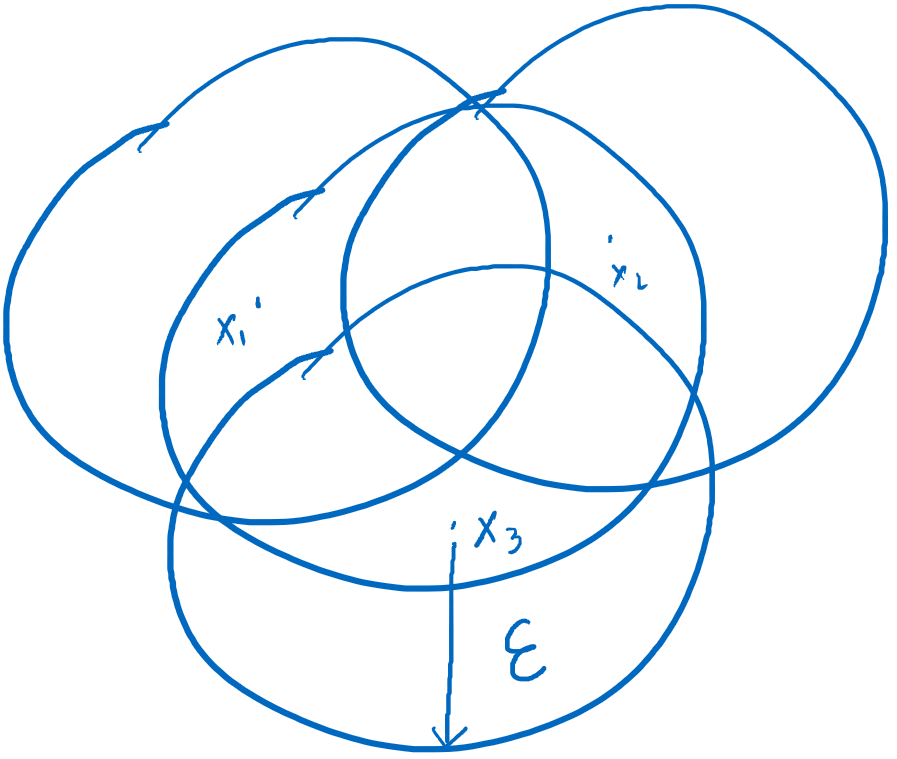
\includegraphics[scale=0.25]{./fig/2.2.3.png}
\end{figure}
显然,全有界集一定是有界集。
\paragraph*{例} \quad $\mathbb{R}^n$中的有界集$\ \Leftrightarrow \ $全有界集。
\begin{definition}[有限$\varepsilon$-网]
    $\{x_i\}_{i=1}^k$称为$A$的有限$\varepsilon$-网。
\end{definition}
接下来我们来证明另外一半:\\
\textbf{Proof:}(列紧闭$ \ \Rightarrow \ $紧)\\
\textbf{Claim 1 全有界集可分}\\
\textbf{Proof:}设$A$为全有界集,对任意$n \in \mathbb{Z}_+$,存在$A$的有限$\varepsilon$-网$B_n$,不妨取$B_n \subset A$
\[\text{考虑}B=\bigcup_{n=1}^{\infty}B_n \ , \ (\text{想证}\bar{B}=A)\]
\[\forall x \in A \ , \ \varepsilon>0 \ , \ \exists \, n_{\varepsilon}=\left[\frac{1}{\varepsilon}\right]+1 \quad s.t. \quad \exists \, y \in B_{n_{\varepsilon}} \ , \ d(x,y)<\frac{1}{n_{\varepsilon}}<\varepsilon\]
\[\Rightarrow \ B_{\varepsilon}(x) \cap B_{n_{\varepsilon}} \neq \varnothing \ \Rightarrow \ B_{\varepsilon}(x) \cap B \neq \varnothing \ \Rightarrow \ x \in \bar{B} \ \Rightarrow \ A \subset \bar{B} \ \Leftrightarrow \ A\text{可分}\]
\textbf{Q.E.D.}\\
\textbf{Claim 2 距离空间中的列紧集是全有界的}\\
\textbf{Proof:}反证:若列紧的$A$不是全有界的,则存在$\varepsilon_n>0$,$A$没有有限$\varepsilon_n$-网。
\[\forall x_0 \in A \ , \ A-B_{\varepsilon_n}(x_0) \neq \varnothing\]
\[\forall x_1 \in A-B_{\varepsilon_n}(x_0) \ , \ A-\bigcup_{i=0}^1B_{\varepsilon_n}(x_i) \neq \varnothing\]
由归纳得存在点列$\{x_n\}_{n=0}^{\infty} \subset A$不收敛$(\forall i \neq j \ , \ d(x_i,x_j)>\varepsilon_n)$,即$A$中点列不全有收敛子列,与题设矛盾。\\
\textbf{Q.E.D.}\\
\textbf{Claim 3 距离空间中的子集是全有界的,那子集的任一开覆盖必有有限子覆盖}\\
\textbf{Proof:}设$A$为全有界集,由引理1可得$A$是可分的,我们设$A$的稠密可数子集为$S$
\[\text{假设有开覆盖}A \subset \bigcup_{\alpha}G_{\alpha} \ , \ \forall x \in A \ , \ \exists \, \alpha \ , \quad s.t. \quad x \in G_{\alpha}(\text{开集}) \ \Rightarrow \ \exists \,r>0 \ , \quad s.t. \quad B_r(x) \subset G_{\alpha}\]
\[B_{\frac{1}{4}r}(x) \cap S \neq \varnothing \ \text{(稠密要求不能有"空洞",不然闭包盖不住全集)} \ \Rightarrow \ y \in B_{\frac{1}{4}r}(x) \cap S\]
\[\text{取}r' \in \left(\frac{r}{4},\frac{r}{2}\right) \cap \mathbb{Q} \ , \ \text{则有} \ x \in B_{r'}(y) \ \text{且} \ B_{r'}(y) \subset B_{r}(x) \subset G_{\alpha}\]
\[\Rightarrow \ A \subset \bigcup_{r' \in \mathbb{Q}}\bigcup_{y \in S}B_{r'(y)}(y) \ \Rightarrow \ A\text{被可数个}B_{r'}(y)\text{覆盖} \ \Rightarrow \ A\text{被可数个}G_{\alpha}\text{覆盖}\]
\textbf{Q.E.D.}\\
下面我们开始正式证明刻画1的另一半:\\
\textbf{Proof (body):}
\[A\text{是列紧闭集,可知}A\text{是全有界的,且其任意开覆盖} \ A \subset \bigcup_{\alpha}G_{\alpha} \ \text{必有可数子覆盖} \ A \subset \bigcup_{i=1}^{\infty}G_{\alpha_i}\]
采用反证法,假设$A$不是紧的,则存在一个$A$的开覆盖无有限子覆盖:
\[\exists \, \{G_{\alpha_i}\}_{i=1}^{\infty} \ , \ \forall n \in \mathbb{Z}_+ \ , \ A \nsubset \bigcup_{i=1}^nG_{\alpha_i} \ \Rightarrow \ \text{取}x_n \in A-\bigcup_{i=1}^nG_{\alpha_i} \ (n=1,2,\cdots)\]
易知,$\forall n \in \mathbb{Z}_+$,$G_{\alpha_n}$中只包含$\{x_n\}$中的有限个点。\\
\[\text{由}A\text{是列紧的闭集可知,} \ \exists \, \{x_{n_k}\}_{k=1}^{\infty} \subset \{x_n\}_{n=1}^{\infty} \ , \quad s.t. \quad \lim_{k \to \infty}x_{n_k}=x \in A\]
\[\Rightarrow \ \exists \, n_0>0 \quad s.t. \quad x \in G_{\alpha_{n_0}} \ \Rightarrow \ \exists \, r>0 \quad s.t. \quad B_r(x) \subset G_{\alpha_{n_0}} \ \Rightarrow \ \exists \, N>0 \quad s.t. \quad k \geq N \ , \ x_{n_k} \in B_r(x)\]
与题设矛盾。\\
\textbf{Q.E.D.}
\begin{theorem}
    完备距离空间中的子集是紧集当且仅当它是全有界闭集。
\end{theorem}
在上一个定理的证明中,我们结合前半部分的证明与后半部分的Claim 2,即证毕该定理的前一半,下面我们只需证明另一部分。其实这里已经可以看出三个条件的强弱:
\[\text{紧}>\text{列紧}>\text{全有界}\]
Proof (完备距离空间中的全有界闭集是紧集):\\
\textbf{Claim 完备距离空间中全有界集是列紧的}\\
\textbf{Proof:}设$A$全有界,$\{x_n\} \subset A$,
\[\exists \, A\text{的有限}1\text{-网}N_1 \ \Rightarrow \ \exists \, x \in N_1 \ , \ B_1(x) \cap \{x_n\}\text{有无限多个点,取其中一个点记作}x_{n_1}\]
\[B_1(x) \cap A\text{也是全有界的} \ , \ \exists \, A\text{的有限}\frac{1}{2}\text{-网}N_2 \ , \ \text{同理取其中一个点记作}x_{n_2}\]
\[\vdots\]
由归纳得
\[\exists \, \{x_{n_k}\}_{k=1}^{\infty} \quad s.t. \quad d(x_{n_k},x_{n_{k+m}})<\frac{1}{2^k} \ \Rightarrow \ \{x_{n_k}\}\text{是柯西列}\]
由完备性,$\exists \, x \in A \quad s.t. \quad x_{n_k} \to x \ , \ (k \to \infty)$。\\
\textbf{Q.E.D.}\\
再由上一个定理后半部分证明的结论可知,距离空间中的列紧闭集是紧集,则证毕。\\
\textbf{Q.E.D.}
\begin{figure}[htbp]
    \center
    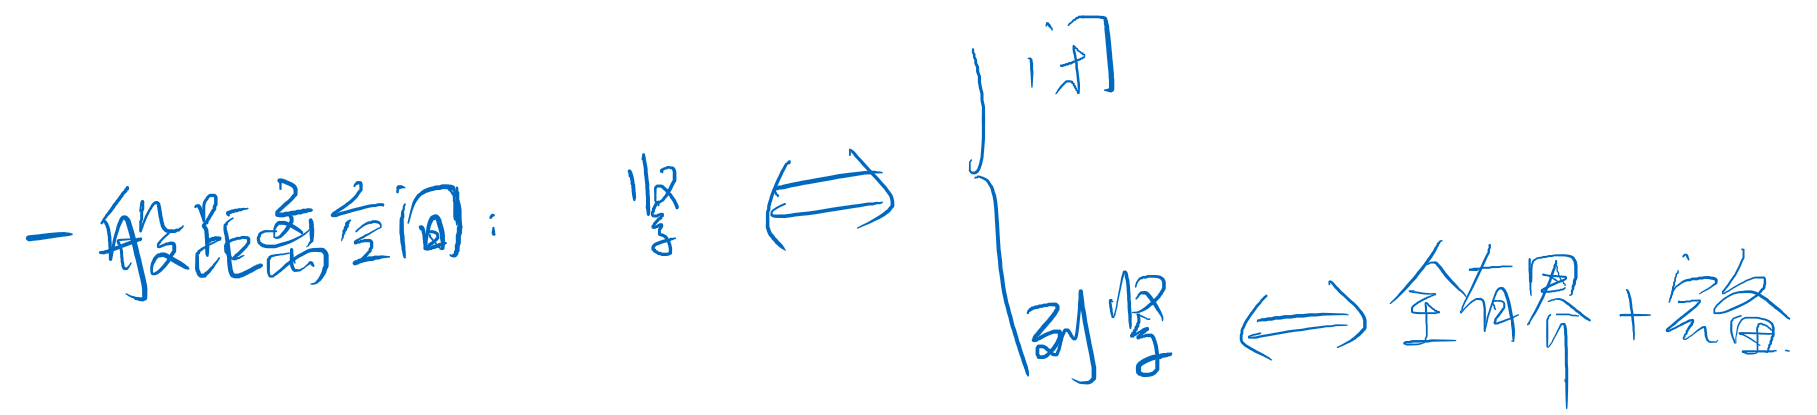
\includegraphics[scale=0.25]{./fig/2.2.3-1.png}
\end{figure}

接下来我们可以看看具体完备距离空间中的(列)紧性的刻画。

\paragraph*{例} \quad $C[a,b]$上的(列)紧性的刻画($Arzela-Ascoli$定理)

为此,我们需要先铺垫一些定义:
\begin{definition}[一致有界]
    $A \subset C[a,b]$,且满足
    \[\exists \, k>0 \ , \ \forall x(t) \in A \ , \ t \in [a,b] \quad s.t. \quad |x(t)| \leq k\]
    则称$A$为一致有界的(与距离空间中的有界是同一回事)。
\end{definition}
\begin{definition}[等度(一致)连续]
    $\forall \varepsilon>0 \ , \ \exists \, \delta>0 \ $,
    \[\forall x(t) \in A \ , \ t_1,t_2 \in [a,b] \ , \ |t_1-t_2|<\delta \quad s.t. \quad |x(t_1)-x(t_2)|<\varepsilon\]
    则称$A$是等度(一致)连续的。
\end{definition}
可以看出,等度(一致)连续是对一族函数的“一致连续”,其$\varepsilon,\delta$的取值与函数无关,容易看出它比一致连续强。

\paragraph*{例1} \quad $\exists \, M>0 \ , \ \forall x(t) \in A \ , \ \forall t \in [a,b] \quad s.t. \quad |x'(t)| \leq M \ $,则$A$是等度连续。\\
\textbf{Proof:}
\[|x(t_1)-x(t_2)|=|x'(\xi)||t_1-t_2| \leq M|t_1-t_2| \quad \xi \in (t_1,t_2) \ : \ |t_1-t_2| \to 0 \ , \ |x(t_1)-x(t_2)| \to 0\]
\textbf{Q.E.D.}

这个命题还能推广,证明也类似。

\paragraph*{例2} \quad $A \subset C^1[a,b]$且$A$在$C^1[a,b]$,则$A$在$C[a,b]$是等度连续。
\begin{theorem}[$Arzela-Ascoli$定理] \label{the:AA}
    $C[a,b]$的子集是列紧的当且仅当它是一致有界且等度连续的。
\end{theorem}
Proof ($C[a,b]$列紧$ \ \Rightarrow \ $全有界$ \ \Rightarrow \ $有界):
\[\forall \varepsilon>0 \ , \ \exists \, A\text{的有限}\frac{\varepsilon}{3}\text{-网}N\text{满足} \ \forall x_i \in N \ , \ \exists \,\delta_i \ , \ t_1,t_2 \in [a,b] \ , \ |t_1-t_2|<\delta_i \quad s.t. \quad |x(t_1)-x(t_2)|<\varepsilon\]
\[\text{取}\delta=\mathop \text{min}\limits_{N}\{\delta_i\} \ , \ \exists \, i \quad s.t. \quad x(t) \subset B_{\frac{\varepsilon}{3}}(x_i(t)) \quad \text{则当}|t_1-t_2|<\delta \ , \ \forall x(t) \in A \ \text{时,有}\]
\[|x(t_1)-x(t_2)| \leq |x(t_1)-x_i(t_1)|+|x_i(t_1)-x_i(t_2)|+|x_i(t_2)-x(t_2)|<\frac{\varepsilon}{3}+\frac{\varepsilon}{3}+\frac{\varepsilon}{3}=\varepsilon\]
\textbf{Q.E.D.}

Proof ($C[a,b]$等度连续,一致有界$ \ \Rightarrow \ $列紧):\\
由于$C[a,b]$完备,故只需证明$C[a,b]$全有界。
\[\forall \varepsilon>0 \ , \ \exists \, \delta>0 \ , \ |t_1-t_2|<\delta \ , \ \forall x(t) \in A \quad s.t. \quad |x(t_1)-x(t_2)|<\varepsilon\]
\[\exists \, k>0 \ , \ \forall x(t) \in A \ , \ t \in [a,b] \quad s.t. \quad |x(t)|<k \quad \text{一致有界}\]
\[\text{取$[-k,k]$划分}:\{y_0,y_1,\cdots,y_n\}:y_0=-k \ , \ y_n=k \ , \ 0<y_{i+1}-y_i<\frac{\varepsilon}{5}\]
\[\text{取$[a,b]$划分}:\{t_0,t_1,\cdots,t_m\}:t_0=a \ , \ t_m=b \ , \ 0<y_{i+1}-y_i<\delta\]
\[\text{若}x(t_i) \in [y_k,y_{k+1}] \ , \ \text{令}f(t_i)=y_k \ , \ \text{其他地方用直线连接,则}\forall t \in [a,b] \ , \ \exists \, t_i \quad s.t. \quad t \in [t_i,t_{i+1}]\]
\begin{figure}[htbp]
    \center
    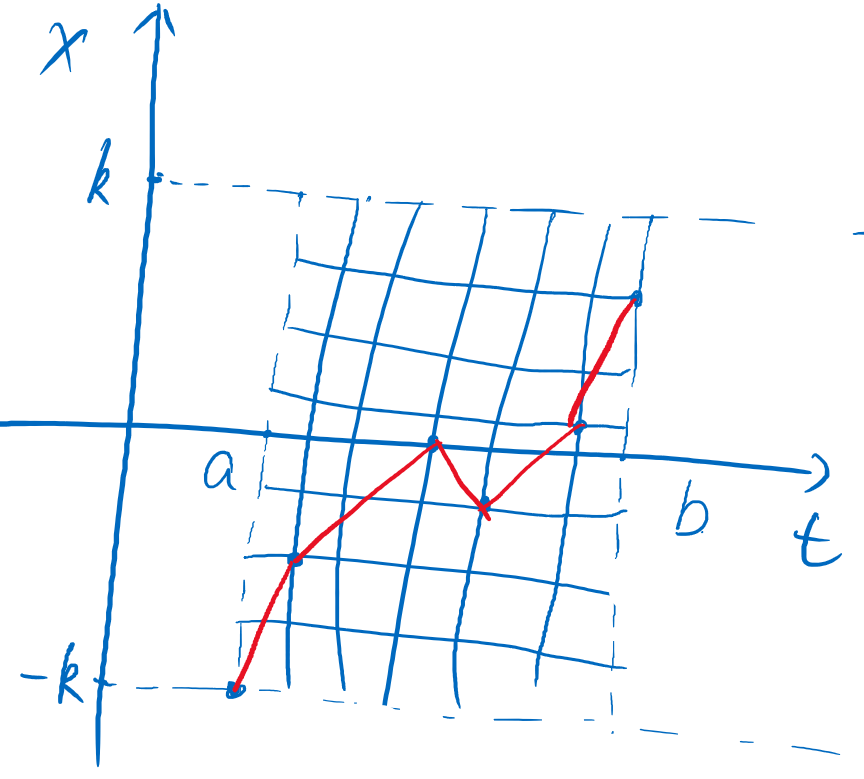
\includegraphics[scale=0.3]{./fig/2.2.3-2.png}
\end{figure}
\[|x(t)-f(t)| \leq |x(t)-x(t_i)|+|x(t_i)-f(t_i)|+|f(t_i)-f(t)|<\frac{\varepsilon}{5}+\frac{\varepsilon}{5}+|f(t_i)-f(t)|\]
\[<\frac{2}{5}\varepsilon+|f(t_i)-f(t_{i+1})|<\frac{2}{5}\varepsilon+|f(t_i)-x(t_i)|+|x(t_i)-x(t_{i+1})|+|x(t_{i+1})-f(t_{i+1})|\]
\[<\frac{2}{5}\varepsilon+\frac{1}{5}\varepsilon+\frac{1}{5}\varepsilon+\frac{1}{5}\varepsilon=\varepsilon\]
\[\text{因$f$至多有限个}(n+1)^{m+1} \ \Rightarrow \ \text{这些$f$构成$A$的一个有限$\varepsilon$-网}\]
\textbf{Q.E.D.}

至此,一般空间的部分我们已经叙述完成,在这一章中我们介绍了距离空间和拓扑空间的一些性质,这些性质将对后续我们叙述具体的距离空间有很大的帮助。
\chapter{赋范线性空间}
\begin{introduction}
    \item $Banach$空间~\ref{Banach}
    \item 有界变差函数~\ref{bounded variation}
    \item $L^p$空间~\ref{lp}
    \item $L^{\infty}$空间~\ref{infty}
    \item 赋范线性空间的基~\ref{baseset}
    \item 有限维赋范线性空间~\ref{the:B}
    \item $Riesz$引理~\ref{Riesz}
  \end{introduction}
\section{赋范线性空间概述}
\subsection{范数,赋范线性空间,$Banach$空间} \label{Banach}
在泛函分析中我们大多处理的都是线性的函数空间,这是基于很多函数空间都是无穷维的线性空间这一事实。
无穷维线性空间区别于有限维线性空间,一些在有限维线性空间中成立的事情在无穷维线性空间中不一定成立:
例如,单位闭球在有限维线性空间中是紧致的但在无穷维线性空间中不一定紧致,这点在上一章的讨论中有证明。

在线性代数中,我们定义过$\mathbb{R}^n$上(有限维线性空间)的模长:
\[\mathbb{R}^n \ : \ \vec{v} \in \mathbb{R}^n \ , \ |\vec{v}|=\sqrt{\sum_{i=1}^nx_i^2}\]

在无限维线性空间我们也同样可以定义类似的概念——范数($norm$)可以看作是模长的推广(其实都是距离空间中的距离)。
\begin{definition}[范数]
    设$X$是定义在$\mathbb{R}$或者$\mathbb{C}$上的线性空间,函数$|| \cdot ||:X \to \mathbb{R}$如果满足\\
    \qquad 1. $\forall x \in X \ , \ ||x|| \geq 0 \ \text{and} \ ||x||=0 \ \text{if and only if} \ x=0 \ $(非负性)\\
    \qquad 2. $\forall x \in X \ , \ \forall a \in \mathbb{R} \ or \ \mathbb{C} \ , \ ||ax||=|a|||x|| \ $(齐次性)\\
    \qquad 3. $\forall x,y \in X \ , \ ||x+y|| \leq ||x||+||y|| \ $(三角不等式)\\
    则称$||\cdot||$是$X$上的一个范数,$(X,||\cdot||)$称为赋范线性空间。
\end{definition}
容易证明,赋范线性空间是距离空间。
\begin{definition}[强收敛(依范数收敛)]
    若$d(x_n,x) \to 0 \ (n \to \infty)$即$||x_n-x|| \to 0 \ (n \to \infty)$,则称$x_n$强收敛于$x$或称依范数收敛。
\end{definition}
我们将完备的赋范线性空间称为$Banach$空间。

同一个集合上可以定义不同的范数:
\[(\mathbb{R}^2,|\vec{x}|) \ , \ |\vec{x}|=\sqrt{x_1^2+x_2^2} \qquad \qquad \qquad (\mathbb{R}^2,|\vec{x}|) \ , \ |\vec{x}|=|x_1|+|x_2|\]
\begin{figure}[H]
    \centering
    \begin{minipage}[t]{0.3\textwidth}
    \centering
    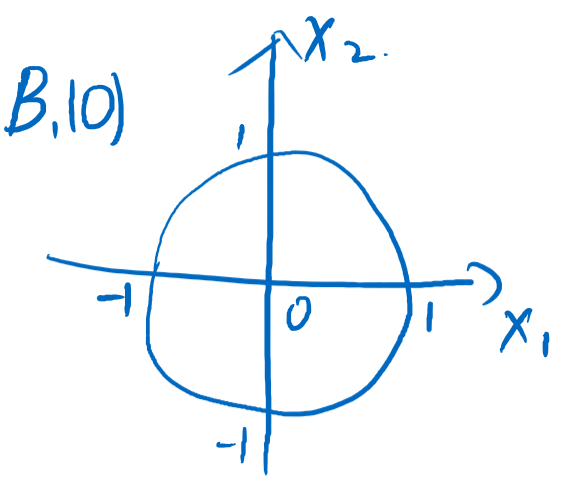
\includegraphics[width=3.5cm]{./fig/3.1.1-1.png}
    \end{minipage}
    \begin{minipage}[t]{0.3\textwidth}
    \centering
    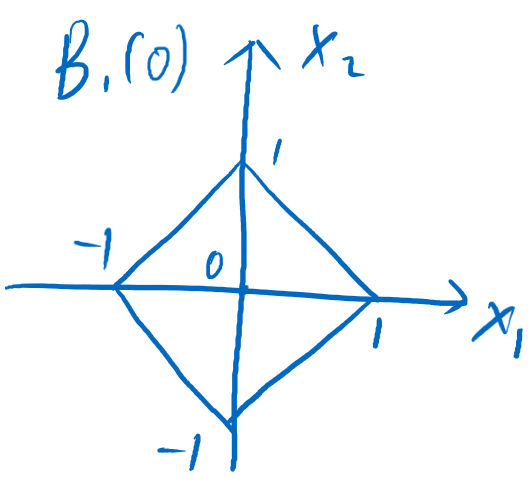
\includegraphics[width=3.5cm]{./fig/3.1.1-2.png}
    \end{minipage}
\end{figure}
下面我们来看几个赋范线性空间的例子。
\paragraph*{例1}$C[a,b] \ , \ ||x(t)||=\mathop \text{sup}\limits_{t \in [a,b]}|x(t)|$是$Banach$空间,无穷维且可分。\\
验证:
\[||x(t)|| \leq 0 \ , \ \text{若}||x(t)||=0 \ \Rightarrow \ \mathop \text{sup}\limits_{t \in [a,b]}|x(t)|=0 \ \Leftrightarrow \ \forall t \in [a,b] \ , \ |x(t)|=0 \ \Rightarrow \ x(t)=0\]
\[||ax(t)||=\mathop \text{sup}\limits_{t \in [a,b]}|ax(t)|=\mathop \text{sup}\limits_{t \in [a,b]}|a||x(t)|=|a|||x(t)||\]
\[||x(t)+y(t)||=\mathop \text{sup}\limits_{t \in [a,b]}|x(t)+y(t)| \leq \mathop \text{sup}\limits_{t \in [a,b]}|x(t)|+\mathop \text{sup}\limits_{t \in [a,b]}|y(t)|=||x(t)||+||y(t)||\]

\paragraph*{例2}$l^{\infty}$是所有有界数列构成的集合,设$X=(x_1,x_2,\cdots)$,设$||X||=\mathop \text{sup}\limits_{i \in \mathbb{N}_+}|x_i|$。容易验证:\\
1、$||\cdot||$是范数; \quad 2、$(l^{\infty},||\cdot||)$是$Banach$空间,无穷维且不可分。

\paragraph*{例3}$L^1[a,b]$是$[a,b]$上所有可积函数(等价类)构成的集合($Lebesgue$积分无法得到严格的相等,只能用等价类来表示,例如若$f=g \ a.e.$,则认为$f$与$g$在$L^1[a,b]$中相同),定义范数
\[||x(t)||_{L^1[a,b]}=\int_a^b|x(t)|\dd t \quad (Lebesgue\text{积分})\]
验证:
\[||x(t)||_{L^1[a,b]}=\int_a^b|x(t)|\dd t \geq 0 \ \text{若}||x(t)||_{L^1[a,b]}=0 \ \Rightarrow \ |x(t)|=0 \ a.e. \ \Rightarrow \ x(t)=0 \ a.e.\]
其余两点容易验证,故$L^1[a,b]$是$Banach$空间。

由此联想,我们也容易想到一个不是$Banach$空间的例子:
\paragraph*{例4}$(C^1[a,b],||\cdot||_{L^1[a,b]})$不完备,故不是$Banach$空间。这件事可以通过范数诱导出的距离加以证明:
\[d(x(t),y(t))=\int_a^b|x(t)-y(t)|\dd t\]

\paragraph*{例5}$V[a,b]$是$[a,b]$上的有界变差函数构成的集合,是$Banach$空间。

当然我们需要先知道有界变差函数是什么。
\begin{definition}[全变差,有界变差函数] \label{bounded variation}
    \[\mathop \text{V}\limits_a^b(x(t))=\mathop \text{sup}\limits_p \sum |x(t_{i+1})-x(t_i)|\]
    其中$p$为$[a,b]$上的任意有限划分$a=t_0<t_1<t_2<\cdots<t_n=b$。\\
    若函数$x(t)$满足
    \[\mathop \text{V}\limits_a^b(x(t))<\infty\]
    则称$x(t)$为有界变差函数。
\end{definition}
首先定义$V[a,b]$上的范数:
\[||x(t)||=|x(a)|+\mathop \text{V}\limits_a^b(x(t))\]
验证其是定义良好的范数:\\
正定性:
\[\text{显然} \ ||x(t)|| \geq 0 \ \text{若} \ ||x(t)||=0 \ \Rightarrow \ x(a)=0 \ \text{且} \ \mathop \text{V}\limits_a^b(x(t))=0 \quad \text{取对半划分:} \ \forall t \in [a,b] \ \text{有:}\]
\[|x(a)-x(t)|+|x(t)-x(b)| \leq \mathop \text{V}\limits_a^b(x(t))=0 \ \Rightarrow \ |x(a)-x(t)|=|x(t)-x(b)|=0 \ \Rightarrow \ x(t)=x(a)=0\]
齐次性显然。\\
三角不等式(注意:这里利用了不等式$\text{sup}(A+B) \leq \text{sup}A+\text{sup}B$)
\[||x(t)+y(t)||=|x(a)+y(a)|+\mathop \text{V}\limits_a^b(x(t)+y(t))=|x(a)+y(a)|+\mathop \text{sup}\limits_p \sum|x_{i+1}(t)-x_i(t)+y_{i+1}(t)-y_i(t)|\]
\[\leq |x(a)|+|y(a)|+\mathop \text{sup}\limits_p \sum|x_{i+1}(t)-x_i(t)|+\mathop \text{sup}\limits_p \sum|y_{i+1}(t)-y_i(t)|=||x(t)||+||y(t)||\]
下面验证$V[a,b]$是$Banach$空间。\\
\textbf{Proof:}\\
设$\{x_n\}$是$V[a,b]$中的柯西列。
\[\forall \varepsilon>0 \ , \ \exists \, N>0 \quad \text{s.t.} \quad n,m \geq N \ , \ ||x_m-x_n||<\varepsilon\]
即对$[a,b]$上的任意有限划分$a=t_0<t_1<t_2<\cdots<t_n=b$都有
\[|x_m(a)-x_n(a)|+\mathop \text{sup}\limits_p \sum |x_m(t_{i+1})-x_n(t_{i+1})-x_m(t_i)+x_n(t_i)|<\varepsilon\]
由此可以得出两件事:一、$\{x_n(a)\}_{n=1}^{\infty}$是柯西列;二、类似的取对半划分:$ \ \forall t \in [a,b] \ $有:
\[|x(a)-x(t)|+|x(t)-x(b)| \leq \mathop \text{V}\limits_a^b(x(t))<\varepsilon \ \Rightarrow \ |x(a)-x(t)|<\varepsilon \ \Rightarrow \ \{x_n(t)-x_n(a)\}_{n=1}^{\infty}\text{是柯西列}\]
有限个柯西列的和还是柯西列,故我们可以得到:$\{x_n(t)\}_{n=1}^{\infty}$是柯西列,即
\[\forall t \in [a,b] \ , \ x_n(t) \xrightarrow{\text{逐点}} x(t)\]
在此基础上,如果我们想进一步证明$x_n(t)$强收敛于$x(t)$,我们需先证明柯西列极限$x(t)$在$V[a,b]$中(利用了有限加和与极限可交换):
\[\mathop \text{V}\limits_a^b(x(t))=x(a)+\mathop \text{sup}\limits_p \lim_{n \to \infty}\sum |x_n(t_{i+1})-x_n(t_i)|=\lim_{n \to \infty} \left ( x_n(a)+\mathop \text{sup}\limits_p \sum |x_n(t_{i+1})-x_n(t_i)| \right )\]
因为$\{x_n(t)\}_{n=1}^{\infty}$是$V[a,b]$中的柯西列,故$\{x_n(t)\}_{n=1}^{\infty}$是$V[a,b]$中的有界集:
\[\forall n \in \mathbb{N}_+ \ , \ \exists \, M>0 \quad \text{s.t.} \quad ||x_n(t)|| \leq M \ \Rightarrow \ \mathop \text{V}\limits_a^b(x(t)) \leq M \ \Leftrightarrow \ \mathop \text{V}\limits_a^b(x(t)) \in V[a,b]\]
下面我们可以开始证明$x_n(t)$强收敛于$x(t)$:
\[||x_n(t)-x(t)||=|x_n(a)-x(a)|+\mathop \text{sup}\limits_p \sum |x_n(t_{i+1})-x(t_{i+1})-x_n(t_i)+x(t_i)|\]
$\exists \, N>0$当$n>N$时:
\[|x_n(a)-x(a)|=\lim_{m \to \infty}|x_n(a)-x_m(a)|<\varepsilon\]
对任意划分$p$:
\[\mathop \text{sup}\limits_p \sum |x_n(t_{i+1})-x(t_{i+1})-x_n(t_i)+x(t_i)|=\lim_{m \to \infty}\mathop \text{sup}\limits_p \sum |x_n(t_{i+1})-x_m(t_{i+1})-x_n(t_i)+x_m(t_i)|\]
\[\leq \lim_{m \to \infty}\mathop \text{sup}\limits_p \sum |x_n(t_{i+1})-x_n(t_i)|+\lim_{m \to \infty}\mathop \text{sup}\limits_p \sum |x_m(t_{i+1})-x_m(t_i)|<\varepsilon+\varepsilon=2\varepsilon\]
\[\Rightarrow \ \forall \varepsilon>0 \ , \ \exists \, N>0 \quad \text{s.t.} \quad n>N \ , \ ||x_n(t)-x(t)||<3\varepsilon \ \Leftrightarrow \ x_n \to x \ (n \to \infty)\]
\textbf{Q.E.D.}

赋范线性空间中一般用$x_n \to x \ (n \to \infty)$表示强收敛。

\subsection{赋范线性空间的基本性质}
下面我们来看一些赋范线性空间的基本性质:
\begin{theorem}
    设$(X,||\cdot||)$是线性赋范空间,则:\\
    1. 范数是连续函数,即$x_n \to x \ \Rightarrow \ ||x_n|| \to ||x|| \ (n \to \infty)$\\
    2. 线性运算是连续映射\\
    i) \ \ $x_n \to x \ , \ y_n \to y \ \Rightarrow \ x_n+y_n \to x+y$\\
    ii) \ $x_n \to x \ , \ a_n \to a \ (\in \mathbb{R} \ or \ \mathbb{C}) \ \Rightarrow \ a_nx_n \to ax$
\end{theorem}
\textbf{Proof}\\
(1):
\[||x_n||=||x_n-x+x|| \leq ||x_n-x||+||x|| \ \Rightarrow \ ||x_n||-||x|| \leq ||x_n-x||\]
\[||x||=||x-x_n+x_n|| \leq ||x-x_n||+||x_n|| \ \Rightarrow \ ||x||-||x_n|| \leq ||x_n-x||\]
\[\Rightarrow \ \text{\Large|} ||x||-||x_n|| \text{\Large|} \leq ||x_n-x|| \to 0 \ (n \to \infty) \ \Rightarrow \ ||x_n|| \to ||x|| \ (n \to \infty)\]
(2.i):
\[||x_n+y_n-x-y|| \leq ||x_n-x||+||y_n-y|| \to 0\]
(2.ii):
\[||a_nx_n-ax|| \leq ||a_nx_n-ax_n+ax_n-ax|| \leq ||a_nx_n-ax_n||+||ax_n-ax||\]
\[=|a_n-a|||x_n||+|a|||x_n-x|| \to 0\]
\textbf{Q.E.D.}

在线性空间中可以利用加法定义级数,赋范线性空间中当然也可以定义级数:
\begin{definition}[级数,部分和,级数收敛]
    设赋范线性空间中的函数列$\{x_n\}_{n=1}^{\infty}$,定义级数为
    \[\sum_{n=1}^{\infty}x_n=x_1+x_2+x_3+\cdots\]
    定义部分和$S_n$
    \[S_n=\sum_{i=1}^nx_i-x_1+x_2+\cdots+x_n\]
    \[\text{若} \ S_n \to S \ (n \to \infty) \ , \ \text{则称级数} \ \sum_{n=1}^{\infty}x_n \ \text{收敛}\]
\end{definition}
\begin{theorem}
    \[(X,||\cdot||) \ \text{是$Banach$空间,级数} \ \sum_{n=1}^{\infty}||x_n|| \ \text{收敛,则} \ \sum_{n=1}^{\infty}x_n \ \text{收敛且} \ \left\| \sum_{n=1}^{\infty}x_n \right\| \leq \sum_{n=1}^{\infty}||x_n||\]
\end{theorem}
\textbf{Proof:}
\[\text{部分和的模长} \ ||S_j||=\left\| \sum_{n=1}^jx_n \right\| \leq \sum_{n=1}^j||x_n||\]
\[\text{由} \ \sum_{n=1}^{\infty}||x_n|| \ \text{收敛} \ \Leftrightarrow \ \forall \varepsilon>0 \ , \ \exists \, N>0 \quad \text{s.t.} \quad j>i \geq N \ , \ \sum_{n=i}^j||x_n||<\varepsilon\]
\[\Rightarrow \ ||S_{j+1}-S_{i-1}||=\sum_{n=i}^j||x_n||<\varepsilon\]
可知部分和序列$\{S_n\}_{n=1}^{\infty}$是柯西列,即$\exists \, S \in X \quad \text{s.t.} \quad S_n \to S \ (n \to \infty)$
\[\text{即} \ \sum_{n=1}^{\infty}x_n \ \text{收敛}\]
进而,由范数$||\cdot||$的连续性,对不等式两边取极限即证毕。
\[\left\| \sum_{n=1}^jx_n \right\| \leq \sum_{n=1}^j||x_n|| \ \Rightarrow \ \left\| \sum_{n=1}^{\infty}x_n \right\| \leq \sum_{n=1}^{\infty}||x_n||\]
\textbf{Q.E.D.}

我们也可以看看赋范线性空间下凸集的性质。
\begin{definition}[凸集]
    设$X$是线性空间,集合$A$满足
    \[A \subset X \ , \ \forall x,y \in A \ , \ t \in (0,1) \quad \text{s.t.} \quad tx+(1-t)y \in A\]
    则称$A$为凸集。
\end{definition}
几何直观:
\begin{figure}[htbp]
    \center
    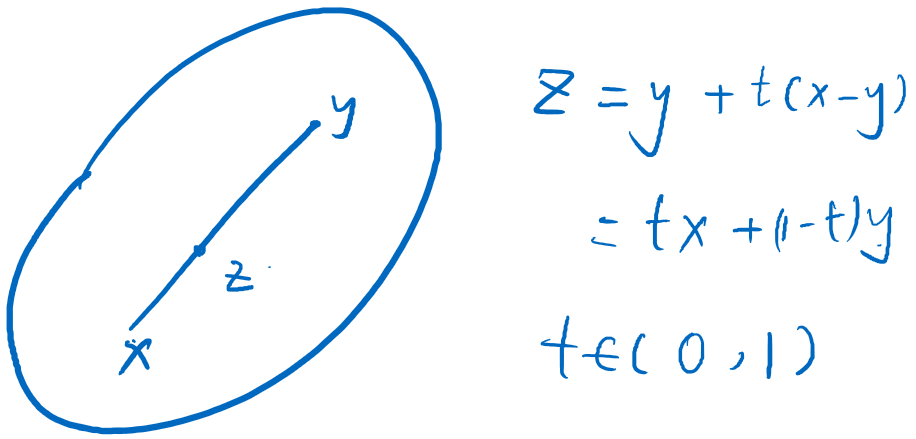
\includegraphics[scale=0.22]{./fig/3.1.2.png}
\end{figure}
\begin{theorem}
    设$(X,||\cdot||)$是赋范线性空间,原点的球邻域$B_r(0)$是凸集。
\end{theorem}
\textbf{Proof:} $B_r(0)=\{x|x \in X \ ,||x||<r\}$,设$x,y \in B_r(0) \ , \ t \in (0,1)$
\[||tx+(1-t)y|| \leq ||tx||+||(1-t)y||=|t|||x||+|1-t|||y||<tr+(1-t)r=r \ \Rightarrow \ tx+(1-t)y \in B_r(0)\]
\textbf{Q.E.D.}
\begin{proposition}
    $(X,||\cdot||)$中任意球是凸集。
\end{proposition}
凸集还有其他基本性质,如任意个凸集的交集是凸集,具体的例子就是赋范线性空间中任意个球的交集是凸集。

关于凸集的性质也有与不动点定理相关的,下面我们简要叙述一下该定理。
\begin{theorem}[$Schauder$不动点定理]
    设$X$是$Banach$空间,$A \subset X$是紧凸集,$T:A \to A$是连续映射,则$T$有不动点(不一定唯一,例如恒等映射)。
\end{theorem}
\paragraph*{例} \quad $T:[0,1] \to [0,1]$
\begin{figure}[htbp]
    \center
    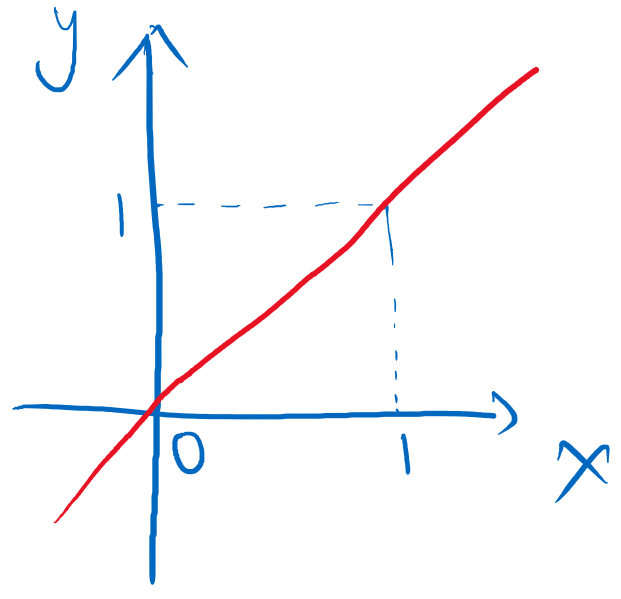
\includegraphics[scale=0.2]{./fig/3.1.2-1.png}
\end{figure}
不动点在$y=x$上,连续映射保证了任意一个$T$都必然与$y=x$有交点。

下面我们将要详细讨论一个赋范线性空间的例子:$L^p(E)$空间 $(p \geq 1)$。

\section{$L^p$空间} \label{lp}
出于方便,我们讨论$L^p$空间的时候都假设$E$是$\mathbb{R}$上的可测集。$L^p$空间定义为
\[L^p(E)=\left\{x(t) \ \text{可测} \ , \ \int_E|x(t)|^p<+\infty\right\}\]
这里$x(t)$是等价类,为方便书写取一代表元,这里$x(t) \sim y(t)$当且仅当$x(t)=y(t) \ a.e. \quad (t \in E)$,在这个集合上我们定义范数:
\[||x(t)||_{L^p(E)}=\left(\int_E|x(t)|^p\dd t\right)^{\frac{1}{p}}\]
验证:\\
\textbf{1、正定性}
\[||x(t)|| \geq 0 \ \text{显然,若}||x(t)||=0 \ \Rightarrow \ \int_E|x(t)|^p\dd t=0 \ \text{,不妨设} \ mE>0 \ \Rightarrow \ x(t)=0 \ a.e.\]
\textbf{2、齐次性}
\[||kx(t)||=\left(\int_Ek|x(t)|^p\dd t\right)^{\frac{1}{p}}=\left(|k|^p\int_E|x(t)|^p\dd t\right)^{\frac{1}{p}}=|k|\left(\int_E|x(t)|^p\dd t\right)^{\frac{1}{p}}\]
\textbf{3、三角不等式}: $Minkowski$不等式\\
要证明上述不等式,我们需要一些其他的基础不等式:
\begin{theorem}[$Young$不等式]
    \[\text{若} \forall p,q>0 \ \text{满足} \ \frac{1}{p}+\frac{1}{q}=1 \ \text{,则对} \ \forall a,b>0 \ \text{都有} \ |ab| \leq \frac{|a|^p}{p}+\frac{|b|^q}{q}\]
\end{theorem}
\textbf{Proof:}不妨设$a,b>0$
\[\frac{1}{p}+\frac{1}{q}=1 \ \Leftrightarrow \ \frac{q}{p}+1=q \ \Leftrightarrow \ 1-q=-\frac{q}{p}\]
\[|ab| \leq \frac{|a|^p}{p}+\frac{|b|^q}{q} \ \Leftrightarrow \ ab^{1-q} \leq \frac{1}{p}\left(\frac{a^p}{b^q}\right)+\frac{1}{q} \ \Leftrightarrow \ \left(\frac{a^p}{b^q}\right)^{\frac{1}{p}}-1 \leq \frac{1}{p}\left(\frac{a^p}{b^q}-1\right)\]
令$t=a^p/b^q>0$,则只需证
\[t^{\frac{1}{p}}-1 \leq \frac{1}{p}(t-1) \quad (t>0 \ ,p>0)\]
令
\[f(t)=t^{\frac{1}{p}}-\frac{1}{p}t-1+\frac{1}{p} \quad (t>0 \ ,p>0)\]
则
\[f'(t)=\frac{1}{p}t^{\frac{1}{p}-1}-\frac{1}{p}=\frac{1}{p}\left(t^{\frac{1}{p}-1}-1\right)\]
易证明$x=1$为$f(x)$的极大值点:
\[f(x) \leq f(1)=0 \ \Rightarrow \ t^{\frac{1}{p}}-1 \leq \frac{1}{p}(t-1) \quad (t>0 \ ,p>0)\]
原命题得证。

\textbf{Q.E.D.}

在使用$Young$不等式的时候我们可以用到一下小技巧:
\[\text{若} \forall p,q>0 \ \text{满足} \ \frac{1}{p}+\frac{1}{q}=1 \ \text{,则对} \ \forall a,b>0 \ , \ \forall \varepsilon>0 \ \text{都有} \ |ab|=|\varepsilon a \cdot \frac{1}{\varepsilon}b| \leq \varepsilon^p\frac{|a|^p}{p}+\frac{1}{\varepsilon^q}\frac{|b|^q}{q}\]
由于$\varepsilon$的任意性,可以用这种小技巧将一些性质不好的项(我不喜欢的项)压住。
\begin{theorem}[$H\ddot{o}lder$不等式]
    设$E$是可测集,$x(t),y(t)$是$E$上的可测函数,则有
    \[\int_E|x(t)y(t)|\dd t \leq \left(\int_E|x(t)|^p\dd t\right)^{\frac{1}{p}}\left(\int_E|y(t)|^q\dd t\right)^{\frac{1}{q}} \quad (p,q>0 \ , \ \frac{1}{p}+\frac{1}{q}=1)\]
    若$x(t) \in L^p(E) \ , \ y(t) \in L^q(E)$则
    \[\int_E|x(t)y(t)|\dd t \leq ||x(t)||_{L^p(E)}||y(t)||_{L^q(E)}\]
\end{theorem}
\textbf{Proof:}设
\[A=||x(t)||_{L^p(E)}=\left(\int_E|x(t)|^p\dd t\right)^{\frac{1}{p}} \qquad B=||y(t)||_{L^q(E)}=\left(\int_E|y(t)|^q\dd t\right)^{\frac{1}{q}}\]
由$Young$不等式:
\[\frac{|x(t)| \cdot |y(t)|}{A \cdot B} \leq \frac{1}{p}\frac{|x(t)|^p}{A^p}+\frac{1}{q}\frac{|y(t)|^q}{B^q} \ \Rightarrow \ \frac{\int_E|x(t)y(t)|\dd t}{A \cdot B} \leq \frac{1}{p}\frac{\int_E|x(t)|^p\dd t}{A^p}+\frac{1}{q}\frac{\int_E|y(t)|^q\dd t}{B^q}=1\]
\[\Rightarrow \ \int_E|x(t)y(t)|\dd t \leq A \cdot B\]

\textbf{Q.E.D.}

下面我可以来证明$Minkowski$不等式($L^p$空间的三角不等式):
\begin{theorem}[$Minkowski$不等式]
    设$x(t),y(t) \in L^p(E) \ (p \geq 1)$,则有
    \[\left(\int_E|x(t)+y(t)|^p\dd t\right)^{\frac{1}{p}} \leq \left(\int_E|x(t)|^p\dd t\right)^{\frac{1}{p}}+\left(\int_E|y(t)|^p\dd t\right)^{\frac{1}{p}}\]
    即
    \[||x(t)+y(t)||_{L^p(E)} \leq ||x(t)||_{L^p(E)}+||y(t)||_{L^p(E)}\]
\end{theorem}
\textbf{Proof:} $p=1$时,显然;$p>1$时,由$H\ddot{o}lder$不等式:
\[\int_E|x(t)+y(t)|^p\dd t=\int_E|x(t)+y(t)||x(t)+y(t)|^{p-1}\dd t\]
\[\leq \int_E|x(t)||x(t)+y(t)|^{p-1}\dd t+\int_E|y(t)||x(t)+y(t)|^{p-1}\dd t\]
\[\leq \left(\int_E|x(t)|^p\dd t\right)^{\frac{1}{p}}\left(\int_E|x(t)+y(t)|^{q(p-1)}\dd t\right)^{\frac{1}{q}}+\left(\int_E|y(t)|^p\dd t\right)^{\frac{1}{p}}\left(\int_E|x(t)+y(t)|^{q(p-1)}\dd t\right)^{\frac{1}{q}}\]
\[\frac{1}{p}+\frac{1}{q}=1 \ \Leftrightarrow \ p=(p-1)q\]
\[\leq \left(\int_E|x(t)|^p\dd t\right)^{\frac{1}{p}}\left(\int_E|x(t)+y(t)|^{p}\dd t\right)^{1-\frac{1}{p}}+\left(\int_E|y(t)|^p\dd t\right)^{\frac{1}{p}}\left(\int_E|x(t)+y(t)|^{p}\dd t\right)^{1-\frac{1}{p}}\]
\[\Rightarrow \ \left(\int_E|x(t)+y(t)|^p\dd t\right) \cdot \left(\int_E|x(t)+y(t)|^{p}\dd t\right)^{\frac{1}{p}-1} \leq \left(\int_E|x(t)|^p\dd t\right)^{\frac{1}{p}}+\left(\int_E|y(t)|^p\dd t\right)^{\frac{1}{p}}\]
\[\Leftrightarrow \ \left(\int_E|x(t)+y(t)|^{p}\dd t\right)^{\frac{1}{p}} \leq \left(\int_E|x(t)|^p\dd t\right)^{\frac{1}{p}}+\left(\int_E|y(t)|^p\dd t\right)^{\frac{1}{p}}\]

\textbf{Q.E.D.}

\section{$L^p$空间的性质}
\begin{theorem}[$Riesz-Fischer$定理]
    $L^p(E) \ (p \geq 1)$是$Banach$空间。\footnote{这里我们指定$E$是$\mathbb{R}$上的可测集,因为说明这种情况比较简单(懒}
\end{theorem}
\textbf{Proof:} \\
(想法是通过$L^p$中的收敛控制$L^1$的收敛($H\ddot{o}lder$不等式),进而得到柯西列收敛从而证明完备性)
\[\text{设} \ \{x_n(t)\} \ \text{是} \ L^p(E) \ \text{中的柯西列,取子列} \ \{x_{n_k}(t)\} \ \text{满足} \ ||x_{n_{k+l}}-x_{n_k}||<\frac{1}{2^k} \ (k=1,2,3,\cdots)\]
(做法是
\[\forall k,m>0 \ , \ \exists \, n_k>0 \quad \text{s.t.} \quad n_{k}>n_{k-1} \ , \ ||x_{n_k+m}-x_{n_k}||<\frac{1}{2^k} \ \Rightarrow \ \text{子列} \ \{x_{n_k}(t)\} \ \text{满足要求}\]
)\\
在下面的讨论中我们需要用到$m(E)<+\infty$这个条件,但是这并不是总能满足的,所有我们取可测集$E_1 \subset E \ , \ m(E_1)<+\infty$,由$H\ddot{o}lder$不等式:
\[\int_{E_1}|x_{n_{k+1}}(t)-x_{n_k}(t)|\dd t \leq \left(\int_{E_1}1^q\dd t\right)^{\frac{1}{q}}\left(\int_{E_1}|x_{n_{k+1}}(t)-x_{n_k}(t)|^p\right)^{\frac{1}{p}}\]
\[\leq \left[m(E_1)\right]^{\frac{1}{q}}||x_{n_{k+1}}(t)-x_{n_k}(t)||_{L^p(E_1)} \leq \left[m(E_1)\right]^{\frac{1}{q}}\frac{1}{2^k}\]
由$Fatou$引理:
\[\Rightarrow \ \int_{E_1} \lim_{n \to \infty}\sum_{k=1}^n|x_{n_{k+1}}(t)-x_{n_k}(t)|\dd t \leq \lim_{n \to \infty} \int_{E_1} \sum_{k=1}^n|x_{n_{k+1}}(t)-x_{n_k}(t)|\dd t \leq \left[m(E_1)\right]^{\frac{1}{q}}\sum_{k=1}^{\infty}\frac{1}{2^k}<\infty\]
\[\Rightarrow \ \sum_{k=1}^{\infty}|x_{n_{k+1}}(t)-x_{n_k}(t)| \ \text{在} \ E_1 \ \text{上} \ a.e. \ \text{收敛}\]
我们知道以下两个事实:1、$E$可以写成可数个有限测度的子集的并集;2、由可列可加性保证可数个零测集的并集还是零测集。
\[\Rightarrow \ \sum_{k=1}^{\infty}|x_{n_{k+1}}(t)-x_{n_k}(t)| \ \text{在} \ E \ \text{上} \ a.e. \ \text{收敛}\]
\[\Rightarrow \ x_{n_l}(t)=x_{n_1}(t)+\sum_{k=1}^{l-1}\left(x_{n_{k+1}}(t)-x_{n_k}(t)\right) \leq x_{n_1}(t)+\sum_{k=1}^{l-1}|x_{n_{k+1}}(t)-x_{n_k}(t)| \ \text{在} \ E \ \text{上} \ a.e. \ \text{收敛}\]

记$x_{n_l}(t)$极限为$x(t)$,柯西列得到的是逐点收敛,为了证明完备性,下面要证明的自然是$x(t) \in L^p(E)$且$x_{n_l}(t) \to x(t) \ (l \to \infty)$,由$Fatou$引理(也可以用控制收敛定理)及柯西列的有界性:
\[\int_E|x(t)|^p\dd t=\int_E\lim_{l \to \infty}|x_{n_l}(t)|^p\dd t \leq \lim_{l \to \infty}\int_E|x_{n_l}(t)|^p\dd t=\lim_{l \to \infty}||X_{n_l}(t)||^p_{L^p(E)}<+\infty\]
即$x(t) \in L^p(E)$。
\[||x_{n_k}(t)-x(t)||^p_{L^p(E)}=\int_E|x_{n_k}(t)-x(t)|^p\dd t=\int_E\lim_{l \to \infty}|x_{n_k}(t)-x_{n_l}(t)|^p\dd t\]
\[\leq \lim_{l \to \infty}\int_E|x_{n_k}(t)-x_{n_l}(t)|^p\dd t=\lim_{l \to \infty}||x_{n_k}(t)-x_{n_l}(t)||^p_{L^p(E)} \leq \left(\frac{1}{2^k}\right)^p \to 0 \ (k \to \infty)\]
即$x_{n_k}(t) \to x(t) \ (k \to \infty)$

\textbf{Q.E.D.}
\begin{theorem}
    $L^p(E) \ (p \geq 1)$是可分的。
\end{theorem}
\textbf{Proof} (只证明$E=[a,b]$的情形,其他的不太好证):\\
想法:逐步逼近(用$\Leftarrow$表示逼近):
\[L^p \ \Leftarrow \ \text{有界}L^p \ \Leftarrow \ \text{连续函数} \ \Leftarrow \ \text{多项式} \ \Leftarrow \ \text{有理多项式}\]
(i) 设$x(t) \in L^p(E)$,令
\[x_n(t)=\left \{
\begin{array}{ll}
    x(t) & , \ |x(t)| \leq n \\ 0 & , \ |x(t)|>n
\end{array}
\right.
\]
\[\int_E|x(t)|^p\dd t=\sum_{n=1}^{\infty} \ \int\limits_{E \cap \{n<|x(t)| \leq n+1\}}|x(t)|^p\dd t<\infty\]
\[\Rightarrow \ \forall \varepsilon>0 \ , \ \exists \, N>0 \quad \text{s.t.} \quad n \geq N \ , \ \int\limits_{E \cap \{|x(t)|>n\}}|x(t)|^p\dd t<\left(\frac{\varepsilon}{3}\right)^p\]
\[\Rightarrow \ ||x_n(t)-x(t)||_{L^p(E)}=\left(\int_E|x_n(t)-x(t)|^p\dd t\right)^{\frac{1}{p}}=\left( \ \int\limits_{E \cap \{|x(t)|>n\}}|x(t)|^p\dd t\right)^{\frac{1}{p}}<\left(\frac{\varepsilon}{3}\right)^{p \cdot \frac{1}{p}}=\frac{\varepsilon}{3}\]
(ii) 取定一个$n \geq N$,由$Lusin$定理:
\[\exists \, y(t) \in C[a,b] \ , \ \mathop \text{sup}\limits_{t \in [a,b]}|y(t)| \leq 2n \quad \text{s.t.} \quad m(\{y(t) \neq x(t)\} \cap E)<\left(\frac{\varepsilon}{3}\right)^p \cdot \frac{1}{(3n)^p}\]
\[(\text{可取上述$|y(t)|$的理由:} \ y(t) \in C[a,b] \ \Rightarrow \ \mathop \text{min}\limits_{t \in [a,b]}\{y(t),2n\} \in C[a,b]\]
\[\text{且} \ |x_n(t)| \leq n \ \Rightarrow \ m(\{y(t)=x_n(t)\})\text{不受影响})\]
\[\Rightarrow \ ||x_n(t)-y(t)||_{L^p(E)}=\left(\int_E|x_n(t)-y(t)|^p\dd t\right)^{\frac{1}{p}}=\left( \ \int\limits_{E \cap \{x_n(t) \neq y(t)\}}|x_n(t)-y(t)|^p\dd t\right)^{\frac{1}{p}}\]
\[\leq \left( \ \int\limits_{E \cap \{x_n(t) \neq y(t)\}}(n+2n)^p\dd t\right)^{\frac{1}{p}} \leq \left(\left(\frac{\varepsilon}{3}\right)^p \cdot \frac{1}{(3n)^p} \cdot (3n)^p\right)^{\frac{1}{p}}=\frac{\varepsilon}{3}\]
(iii) 由$Weierstrass$定理,存在有理系数多项式$P(t)$使得
\[\mathop \text{sup}\limits_{t \in [a,b]}|P(t)-y(t)|<\frac{\varepsilon}{3m(E)^{\frac{1}{p}}}\]
\[||P(t)-y(t)||_{L^p(E)}=\left(\int_E|P(t)-y(t)|^p\dd t\right)^{\frac{1}{p}} \leq \left(m(E) \cdot \frac{\varepsilon^p}{3^pm(E)}\right)^{\frac{1}{p}}=\frac{\varepsilon}{3}\]
由三角不等式
\[||P(t)-x(t)||_{L^p(E)} \leq ||P(t)-y(t)||_{L^p(E)}+||y(t)-x_n(t)||_{L^p(E)}+||x_n(t)-x(t)||_{L^p(E)}<\varepsilon\]
由$\varepsilon$的任意性,得$||P(t)-x(t)||_{L^p(E)} \to 0$。即有理多项式集合在$L^p(E)$中稠密,即$L^p(E)$可分。

\textbf{Q.E.D.}

在这$Riesz-Fischer$定理的证明中,我们有提到过不同范数之间的强弱,我们下面对这件事进行以下严格地叙述。

设$m(E)<\infty \ , \ p_1<p_2$,由$H\ddot{o}lder$不等式:
\[\left(\int_E|x(t)|^{p_1}\dd t\right)^{\frac{1}{p_1}} \leq \left[\left(\int_E\left(|x(t)|^{p_1}\right)^{\frac{p_2}{p_1}}\dd t\right)^{\frac{p_1}{p_2}}\left(\int_E1^{\frac{p_2}{p_2-p_1}}\dd t\right)^{1-\frac{p_1}{q_2}}\right]^{\frac{1}{p_1}}\]
\[\leq \left(\int_E|x(t)|^{p_2}\dd t\right)^{\frac{1}{p_2}} \cdot m(E)^{\frac{1}{p_1}-\frac{1}{p_2}}\]
\[\text{即} \ x(t) \in L^{p_2}(E) \ \Rightarrow \ x(t) \in L^{p_1}(E) \ \text{即} \ L^{p_2}(E) \subset L^{p_1}(E) \ (p_2>p_1)\]

我们自然会好奇,当上面这个性质当$p \to \infty$时成立吗?下面我们来看看$L^{\infty}(E)$空间。我们先引入一些辅助概念来定义$L^{\infty}(E)$空间。
\begin{definition}[本质有界]
    若存在零测集$E_0 \ , \ m(E_0)=0$使$x(t)$在$E/E_0$上有界,则称$x(t)$在$E$上本质有界($essentially \ bounded$)。
\end{definition}
我们将$L^{\infty}(E)$空间定义为:
\[L^{\infty}(E)=\left\{E\text{上本质有界的可测函数构成的集合}\right\}\]
并且定义$L^{\infty}(E)$范数:
\[||x(t)||_{L^p(E)}=\mathop \text{inf}\limits_{\substack{E_0 \subset E \\ m(E_0)=0}}\mathop \text{sup}\limits_{E/E_0}|x(t)|\]
可以验证$||x(t)||_{L^p(E)}$也是范数。我们可以证明,$||x(t)||_{L^p(E)}<\infty \ \Leftrightarrow \ $本质有界。\\
\textbf{Proof:} 若$x(t)$本质有界,则$\exists \, E_0 \quad \text{s.t.} \quad E/E_0$上$|x(t)|$有界$ \ \Rightarrow \ ||x(t)||_{L^{\infty}(E)}<\infty$。\\
反之,由下确界的性质有:
\[\forall n \in \mathbb{Z}_+ \ , \ \exists \,E_n \subset E \ , \ m(E_n)=0 \quad \text{s.t.} \quad \mathop \text{sup}\limits_{E/E_n}|x(t)|<||x(t)||_{L^{\infty}(E)}+\frac{1}{n}\]
令
\[E_0=\bigcup_{n=1}^{\infty}E_n \ , \ m(E_n)=0 \ \Rightarrow \ m(E_0)=0 \ \Rightarrow \ \mathop \text{sup}\limits_{E/E_0}|x(t)|<||x(t)||_{L^{\infty}(E)}<\infty\]
那么$x(t)$本质有界。\\
\textbf{Q.E.D.}
\begin{definition}[本质上界] \label{infty}
    我们称$||x(t)||_{L^{\infty}} (E)$为$x(t)$在$E$上的本质上界(确实是对$|x(t)|$而言的)。
\end{definition}
这里我们不加证明的叙述一些$L^{\infty}(E)$空间的性质,如果我们限定$m(E)<+\infty$,则$\forall x(t) \in L^{\infty}(E) \ , \ x(t) \in L^p(E) \ (p \geq 1)$,反之则不然,这也即:
\[L^{\infty}(E) \subset \bigcap_{p \geq p_0}L^{p}(E) \ (\forall p_0 \geq 1)\]
但需要注意
\[L^{\infty}(E) \neq \bigcap_{p \geq p_0}L^{p}(E) \ (\forall p_0 \geq 1)\]
同时我们也容易看出来$||x||_{L^p(E)} \leq ||x||_{L^{\infty}(E)}$,毕竟正常$L^p$范数可以看作是对函数值的p次几何平均,而$L^{\infty}$范数只取了极大值。下面我们可以看一个具体的例子:
\paragraph*{例} \quad $x(t)=\ln t \ , \ t \in (0,1]$,可以验证$x(t) \in L^p(0,1] \ (p \geq 1)$但$x(t) \notin L^{\infty}(E)(0,1]$。

下面我们看看其他$L^{\infty}(E)$空间的性质。
\begin{theorem}
    $(L^{\infty}(E),||\cdot||_{L^{\infty}(E)})$是$Banach$空间。
\end{theorem}
\textbf{Proof:}设$\{x_n(t)\}$是柯西列,则
\[\exists \, \{x_{n_{k}}(t)\} \subset \{x_n(t)\} \quad \text{s.t.} \quad \forall k,l \in \mathbb{N} \ , \ ||x_{n_{k+l}}(t)-x_{n_{k}}(t)||<\frac{1}{2^k}\]
\[\Rightarrow \ \exists \, E_{k,l} \ , \ m(E_{k,l})=0 \quad \text{s.t.} \quad \forall k,l \in \mathbb{N} \ , \ |x_{n_{k+l}}(t)-x_{n_{k}}(t)|<\frac{1}{2^k} \ , \ \forall t \in E/E_{k,l}\]
由可列可加性:
\[E_0=\bigcup_{k,l\in \mathbb{N}}E_{k,l} \ \Rightarrow \ m(E_0)=0\]
\[\Rightarrow \ \forall t \in E/E_0 \quad \text{s.t.} \quad \forall k,l \in \mathbb{N} \ , \ |x_{n_{k+l}}(t)-x_{n_{k}}(t)|<\frac{1}{2^k}\]
\[\Rightarrow \ \forall t \in E/E_0 \quad \text{s.t.} \quad \sum_{k=1}^{\infty}|x_{n_{k+1}}(t)-x_{n_{k}}(t)|<\sum_{k=1}^{\infty}\frac{1}{2^k}=1<+\infty\]
\[\Rightarrow \ x(t):=\lim_{k \to \infty}x_{n_k}(t) \quad \forall t \in E/E_0 \quad \text{s.t.} \quad |x(t)|=\left|x_{n_1}(t)+\sum_{k=1}^{\infty}(x_{n_{k+1}}(t)-x_{n_{k}}(t))\right|<+\infty\]
$\Rightarrow \ x_{n_k}(t) \to x(t) \ (k \to \infty)$,即$x_{n_k}(t)$逐点收敛到$x(t)$,证明完逐点收敛后下证依范数收敛。
\[\forall t \in E/E_0 \quad \text{s.t.} \quad |x_{n_{k+l}}(t)-x_{n_{k}}(t)|<\frac{1}{2^k} \ \Rightarrow \ \mathop \text{sup}\limits_{E/E_0}|x_{n_{k+1}}(t)-x_{n_{k}}(t)| \leq \frac{1}{2^k} \ (\forall l=1,2,\cdots)\]
当$l \to \infty$时,
\[\mathop \text{sup}\limits_{E/E_0}|x(t)-x_{n_{k}}(t)| \leq \frac{1}{2^k} \ (\forall l=1,2,\cdots)\]
\[\Rightarrow \ ||x(t)-x_{n_k}(t)||_{L^{\infty}(E)}=\mathop \text{inf}\limits_{\substack{E_0 \subset E \\ m(E_0)=0}} \mathop \text{sup}\limits_{E/E_0}|x(t)-x_{n_{k}}(t)| \leq \frac{1}{2^k} \ (\forall k=1,2,\cdots)\]
令$k \to \infty \ , \ x_{n_k}(t) \to x(t)$即$x_{n_k}(t)$依范数收敛到$x(t)$。\\
\textbf{Q.E.D.}

$L^p$空间也有离散情形下的例子,在$\mathbb{Z}_+$上考虑计数测度$\mu_c$,数列$x=\{\xi_n\}_{n=1}^{\infty}$可视为$\mathbb{Z}_+$的可测函数,他的积分:
\[\int_{\mathbb{Z}_+}|x|^p\dd\mu_c=\sum_{n=1}^{\infty}|\xi_n|^p\]
我们定义:
\[l^p=\{\{\xi_n\}_{n=1}^{\infty} \ , \ \sum_{n=1}^{\infty}|\xi_n|^p<\infty\} \qquad ||x||_{l^p}=\left(\sum_{n=1}^{\infty}|\xi_n|^p\right)^{\frac{1}{p}}\]
当$p=\infty$时
\[l^{\infty}=\{\{\xi_n\}_{n=1}^{\infty} \ , \ \mathop \text{sup}\limits_{n \in \mathbb{Z}_+}|\xi_n|<\infty\} \qquad ||x||_{l^{\infty}}=\mathop \text{sup}\limits_{n \in \mathbb{Z}_+}|\xi_n|\]
可以证明$l^p \ , \ l^{\infty}$是$Banach$空间。
\paragraph*{$L^p \ , \ L^{\infty}$的应用举例——纳什迭代($Nash-Moser \ iteration$)} \quad \\
$\Delta u=fu \ , \ f$是给定函数 $u:\Omega \subset \mathbb{R}^n \to \mathbb{R}$,若$f \in L^q(\Omega)$,则$\exists \, c>0 \quad \text{s.t.} \quad ||u||_{L^{\infty}(\Omega)} \leq ||u||_{L^p(\Omega)}$

\section{赋范线性空间的其他性质}
\subsection{赋范线性空间的子空间与完备化}
设$(X,||\cdot||)$是赋范线性空间,$X_1$是$X$的子空间,$(X_1,||\cdot||)$是赋范线性空间,则称$(X_1,||\cdot||)$是$(X,||\cdot||)$的一个子空间。
\begin{theorem}
    \paragraph*{1.} 赋范线性空间的完备子空间是$Banach$空间;
    \paragraph*{2.} $Banach$空间的闭子空间是$Banach$空间。
\end{theorem}
\paragraph*{例} $l^{\infty}$是$Banach$空间,$||x||=\mathop \text{sup}\limits_{n \in \mathbb{Z}_+}|\xi_n| \ , \ x=\{\xi_n\}$,记$c=l^{\infty}$中的收敛数列的集合。可证明$c$是$Banach$空间。\\
\textbf{Proof:} 只需证明$c$是$l^{\infty}$的闭子空间。

设$x_n=\{\xi_{n,i}\}_{i=1}^{\infty}$是$c$中的收敛点列,设$x_n \to x=\{\xi_i\}_{i=1}^{\infty}$,需证$x \in c$,即证$\{\xi_i\}_{i=1}^{\infty}$是收敛数列。
\[\forall \varepsilon>0 \ , \ \exists \, N>0 \quad \text{s.t.} \quad n \geq N \ , \ ||x_n-x||_{l^{\infty}}<\varepsilon \ \Rightarrow \ \exists \, N>0 \quad \text{s.t.} \quad n \geq N \ , \ \mathop \text{sup}\limits_{i \in \mathbb{Z}_+}|\xi_{n,i}-\xi_i|<\varepsilon\]
由于$\{\xi_{n,i}\}_{i=1}^{\infty}$是收敛点列,故它是柯西列,则有
\[\forall \varepsilon>0 \ , \ \exists \, I_n>0 \quad \text{s.t.} \quad i,j \geq I_n \ , \ |\xi_{n,i}-\xi_{n,j}|<\varepsilon\]
则当$i,j \geq I_n$时,有
\[|\xi_{i}-\xi_{j}| \leq |\xi_{i}-\xi_{n,1}|+|\xi_{n,i}-\xi_{n,j}|+|\xi_{n,j}-\xi_{j}|<3\varepsilon\]
即$x=\{\xi_i\}_{i=1}^{\infty}$是柯西列且是实数列,故$x$收敛,从而$x \in c$。\\
\textbf{Q.E.D.}

在上述子空间的内容中我们用到了完备赋范线性空间($Banach$空间),我们自然就会关心赋范线性空间如何完备化的。

我们知道,赋范线性空间是一个距离空间,距离空间是可以完备化的,那么我们自然就会去思考,这样完备化得到的距离空间还是不是赋范线性空间呢?为此我们需要验证其线性结构(加法,数乘)、范数。
\begin{theorem}
    设$(X,||\cdot||)$是不完备的赋范线性空间,它作为距离空间有完备化$\tilde{X}$,可以证明$\tilde{X}$是$Banach$空间。
\end{theorem}
\paragraph*{recall} \quad 设$\tilde{x}=[\{x_n\}] \in \tilde{X}$是$X$中柯西列的等价类。
\paragraph*{定义加法} \quad $\tilde{x}+\tilde{y}=[\{x_n+y_n\}]$\\
容易验证: 1.柯西列相加还是柯西列; 2.加法的定义与等价类无关。
\paragraph*{定义数乘} \quad $k\tilde{x}=[\{kx_n\}]$\\
容易验证: 1.柯西列数乘后还是柯西列; 2.数乘的定义与等价类无关。
\paragraph*{定义范数}
\[||\tilde{x}||_{\tilde{X}}=\lim_{n \to \infty}||x_n||_X\]
我们需要验证:1.$\{\tilde{x}_n\}$是柯西列; 2.$||\tilde{x}||_{\tilde{X}}$的取值与代表元的选取无关。\\
我们知道,$\{x_n\}_{n=1}^{\infty} \subset X$是柯西列时,可以得到$\{||x_n||\}_{n=1}^{\infty}$是收敛的柯西列。
\[\forall \varepsilon>0 \ , \ \exists \, N>0 \quad \text{s.t.} \quad \forall m>n \geq N \ , \ ||x_n-x_m||<\varepsilon\]
\[\forall \varepsilon>0 \ , \ \exists \, N>0 \quad \text{s.t.} \quad \forall m>n \geq N \ , \ \left|||x_n||-||x_m||\right| \leq ||x_n-x_m||<\varepsilon\]
当$m \to \infty$时,记$x:=x_m \ (m \to \infty)$:
\[\forall \varepsilon>0 \ , \ \exists \, N>0 \quad \text{s.t.} \quad \forall n \geq N \ , \ \left|||x_n||-||x||\right|<\varepsilon\]
1.即证。

我们定义等价类为$x \mapsto \tilde{x}=[\{x,x,\cdots\}]$,则$x$可嵌入$\tilde{x}$中,则
\[||\tilde{x}||_{\tilde{X}}=\lim_{n \to \infty}||x_n||_X=||x||_X\]
两个范数的定义是一致的,2.也证毕。\\
\textbf{Q.E.D.}

\subsection{商空间与乘积空间}
在有限维空间中,商空间的定义如下,我们先定义$V$是定义在数域$\mathbf{K}$上的一个向量空间:
\begin{definition}[商空间]
    商空间$V/A=\{\tilde{x}=x+A\}$,其中$\tilde{x}$是一个等价类,等价关系$\sim$定义如下:$x \sim y$当且仅当$x-y \in A$。
\end{definition}
再者,我们定义商映射$\pi:V \to V/A \ , \ x \mapsto \tilde{x}$,显然,这是个线性映射且是满射。
\[\text{加法:}\tilde{x}+\tilde{y}=\tilde{x+y} \qquad \text{数乘:}k\tilde{x}=\tilde{kx} \ (x,y \in V \ , \ k \in \mathbb{K})\]
注:有限维的子空间都是闭子空间。

可以看到,商空间其实是我们所熟知的平行这个概念的推广,现在这个空间中的跟某个$x$之差属于$A$的元素$\tilde{x}$视作一个等价类,可以说说$\tilde{x}$跟x只差了一个$A$。

下面我们来看无限维的情况:假设X是赋范线性空间,$M$是$X$的闭子空间,在商空间$X/M$中定义范数
\[||\tilde{x}||=\mathop \text{inf}\limits_{y \in \tilde{x}}||y||=\mathop \text{inf}\limits_{y-x \in M}||y||=\mathop \text{inf}\limits_{z \in M}||x+z||\]
则课称$X/M$是关于$M$的赋范商空间。我们可以验证$||\tilde{x}||$是范数:
\paragraph*{1、正定性} \quad $||\tilde{x}||>0$是显然的,而当
\[||\tilde{x}||=0 \ , \ \exists \, \{y_n\}_{n=1}^{\infty} \subset \tilde{x} \quad \text{s.t.} \quad \lim_{n \to \infty}||y_n||=0\]
而由于$M$是闭子空间,$x+M$也是闭子空间,故$\exists \, y \in \tilde{x} \quad \text{s.t.} \quad y_n \to y \ (n \to \infty)$
\[||y||=\lim_{n \to \infty}||y_n||=0 \ \Rightarrow \ y=0 \ \Rightarrow \ \tilde{x}=\tilde{y}=\tilde{0}\]
\paragraph*{2、齐次性}
\[||k\tilde{x}||=\mathop \text{inf}\limits_{y \in k\tilde{x}=\tilde{kx}}||y||=\mathop \text{inf}\limits_{z \in \tilde{x}}||kz||=|k|\mathop \text{inf}\limits_{z \in \tilde{x}}||z||=|k|||\tilde{x}||\] 
\paragraph*{3、三角不等式} \quad $\tilde{x},\tilde{y} \in X/M$
\[||\tilde{x}+\tilde{y}||=\mathop \text{inf}\limits_{z \in \tilde{x+y}}||z||=\mathop \text{inf}\limits_{z \in M}||x+y+z|| \leq \mathop \text{inf}\limits_{z \in M}\left(||x+\frac{1}{2}z||+||y+\frac{1}{2}z||\right)\]
\[\leq \mathop \text{inf}\limits_{z \in M}||x+\frac{1}{2}z||+||y+\mathop \text{inf}\limits_{z \in M}\frac{1}{2}z||=||\tilde{x}||+||\tilde{y}||\]
关于商空间,我们有以下定理。
\begin{theorem}
    若$X$是$Banach$空间,$M$是$X$的闭子空间,那么$X/M$是$Banach$空间。
\end{theorem}
\textbf{Proof:} 设$\{\tilde{x}_n\}$是$X/M$中的柯西列,取其子列$\{\tilde{x}_{n_k}\}$使得$||\tilde{x}_{n_{k+1}}-\tilde{x}_{n_k}||<1/2^k \ (k=1,2,\cdots)$,由范数的定义:
\[\mathop \text{inf}\limits_{y_k \in \tilde{x}_{n_{k+1}}-\tilde{x}_{n_k}}||y_k||<\frac{1}{2^k} \quad (\forall k \in \mathbb{Z}_+) \quad \Leftrightarrow \quad \exists \, y_k \in \tilde{x}_{n_{k+1}}-\tilde{x}_{n_k} \quad \text{s.t.} \quad ||y_k||<\frac{1}{2^k}\]
\[\Rightarrow \quad \sum_{k=1}^{\infty}y_k \ \text{在$X$中收敛} \quad \Rightarrow \quad x_{n+1}+\sum_{k=1}^{\infty}y_k \ \text{在$X$中收敛,记极限为} \ S\]
记上述级数的部分和为$S_i$,则易知$S_i$在$X$中的收敛
\[S_i=x_{n_1}+\sum_{k=1}^{i-1}y_k\]
则
\[\tilde{S}_i=\tilde{x}_{n_1}+\sum_{k=1}^{i-1}\tilde{y}_k=\tilde{x}_{n_1}+\sum_{k=1}^{i-1}\left(\tilde{x}_{n_{k+1}}-\tilde{x}_{n_k}\right)=\tilde{x}_{n_i}\]
\[\Rightarrow \quad ||\tilde{x}_{n_i}-\tilde{x}||=||\tilde{S}_i-\tilde{x}||=\mathop \text{inf}\limits_{y \in \tilde{S}_i-\tilde{x}}||y|| \leq ||S_i-x||\rightarrow 0 \quad (i \rightarrow \infty)\]
子列收敛,故原柯西列也收敛。

\textbf{Q.E.D.}
\begin{definition}[乘积空间]
    设$(X_1,||\cdot||_{X_1})$与$(X_2,||\cdot||_{X_2})$是赋范线性空间,则称$(X_1 \times X_2,||\cdot||)$为乘积空间,其中范数定义如下
    \[||(x_1,x_2)||=||x_1||_{X_1}+||x_2||_{X_2} \quad (\forall x_1 \in X_1,x_2 \in X_2)\]
\end{definition}
若$(X_1,||\cdot||_{X_1})$与$(X_2,||\cdot||_{X_2})$是$Banach$空间,则$(X_1 \times X_2,||\cdot||)$也为$Banach$空间。

\subsection{赋范线性空间的基} \label{baseset}
对有限维赋范线性空间$X$,如果我们称$\{e_i\}_{i=1}^{\infty} \subset X$为是$X$的一组基,则其应满足
\[\forall x \in X \ , \ \exists \, ! (\xi_1,\xi_2,\cdots,\xi_n) \in \mathbb{R}^n \quad \text{s.t.} \quad x=\sum_{i=1}^n\xi_ie_i\]

类似的,我们也希望基的概念能拓展到无限维的赋范线性空间上来\footnote{毕竟泛函分析又名无穷维线性代数(乐},类似的我们可能会有以下两种想法(然而并不会):
\paragraph*{$Hamel$基}
如果我们保留有限组合这个性质,我们按照如下方式可以定义$Hamel$基:
\begin{definition}[$Hamel$基]
    设无穷维赋范线性空间$X$的线性无关子集为$\{x_{\alpha}\} \ (\alpha \in \Lambda)$,若其张成的空间(称为线性包)满足$\text{Span}\{x_{\alpha}\}=X$,则称$\{x_{\alpha}\}$为$X$的一个$Hamel$基。
\end{definition}
这样的基是有限维赋范线性空间的基的直接推广,它总是存在的(这点可以利用$Zorn$引理证明,但这个结果其实挺显然而且我不关心这个证明所以我不证),但缺点也很明显,就是基的个数可能会太多,这显然会给运算带来很大的麻烦。

于是便有了另外一种基的出现:
\paragraph*{$Schauder$基}
我们将组合的个数适当拓展到至多可数,我们便可按照如下方式定义$Schauder$基:
\begin{definition}[$Schauder$基]
    设无穷维赋范线性空间$X$中的点列$\{e_n\}_{n=1^{\infty}}$若满足
    \[\forall x \in X \ , \ \exists \, !\{\xi_n\}_{n=1}^{\infty} \ (\xi_n \in \mathbb{R}^1) \quad \text{s.t.} \quad x=\sum_{i=1}^{\infty}\xi_ie_i\]
    则称$\{e_n\}_{n=1^{\infty}}$是$X$的一个$Schauder$基。
\end{definition}
当然,从定义可以看出,不是所有赋范线性空间都有$Schauder$基,$Schauder$基的存在要求其赋范线性空间是可分的。
\paragraph*{例1} \quad $l^p \ (p \geq 1) \ , \ e_i=\{0,\cdots,0,1,0,\cdots\}$ (第$i$位为1),可验证$\{e_n\}_{n=1}^{\infty}$是$Schauder$基。
\paragraph*{例2} \quad $L^2[0,2\pi]$可验证$\{1,\cos nx,\sin nx \ (n=1,2,\cdots)\}$是$Schauder$基。

对于$Schauder$基还有以下小结论:
\[x=\sum_{i=1}^{\infty}\xi_ie_i=\lim_{n \to \infty}\sum_{i=1}^{n}\xi_ie_i \quad \Leftrightarrow \quad ||x-\sum_{i=1}^n\xi_ie_i||=||\sum_{i=n+1}^{\infty}\xi_ie_i|| \rightarrow 0 \quad (n \rightarrow 0) \quad \Rightarrow \quad \xi_i \rightarrow 0 \ (i \to \infty)\]
该结论可以用于快速判断某些点列是不是$Schauder$基,同时,这其实也暗示了可分的赋范线性空间其实“维数”也并不是很多。
\paragraph*{例1} \quad $l^{\infty} \ , \ e_i=\{0,\cdots,0,1,0,\cdots\}$ (第$i$位为1),$\{e_n\}_{n=1}^{\infty}$不是$Schauder$基。

这是显然的,因为该点列末端并不$\to 0$。
\begin{theorem}
    $Banach$空间$X$有$Schauder$基,则$X$可分。
\end{theorem}
\textbf{Proof:}
\[\text{令}A=\left\{\left.x=\sum_{i=1}^nr_ie_i\right|r_i \in \mathbb{Q} \ , \ n \in \mathbb{N}\right\}\text{,则$A$是可数集}\]
下证$A$在$X$中稠密,即:
\[\forall \varepsilon>0 \ , \ x \in X \ , \ x=\sum_{i=1}^{\infty}\xi_ie_i \quad \Leftrightarrow \quad \lim_{n \to \infty}||x-\sum_{i=1}^n\xi_ie_i||=0 \quad \Leftrightarrow \quad \exists \, N \in \mathbb{N} \quad \text{s.t.} \quad ||x-\sum_{i=1}^N\xi_ie_i||<\frac{\varepsilon}{2}\]
容易看出:
\[\exists \, r_1,r_2,\cdots,r_N \in \mathbb{Q} \ , \ y=\sum_{i=1}^Nr_ie_i \in A \quad \text{s.t.} \quad ||y-\sum_{i=1}^N\xi_ie_i||=||\sum_{i=1}^N(r_i-\xi_i)e_i|| \leq \sum_{i=1}^N|r_i-\xi_i|\cdot||e_i||\]
利用$Schwartz$不等式:
\[\sum_{i=1}^N|r_i-\xi_i|\cdot||e_i|| \leq \sqrt{\sum_{i=1}^N|r_i-\xi_i|^2} \cdot \sqrt{\sum_{i=1}^N||e_i||^2} \leq N \cdot \mathop \text{max}\limits_i||e_i|| \cdot \mathop \text{max}\limits_i|r_i-\xi_i|<\frac{\varepsilon}{2}\]
故有
\[||x-y|| \leq ||x-\sum_{i=1}^N\xi_ie_i||+||y-\sum_{i=1}^N\xi_ie_i||<\varepsilon\]

\textbf{Q.E.D.}

但是反之并不一定成立,可分的$Banach$空间并不一定有$Schauder$基。
\vspace{0.5cm}
同一个空间可以定义不同的范数,也即不同的距离函数,那我们自然而然地会想问不同距离函数之间是否有关系,他们的收敛性如何让,拓扑关系如何?
\begin{definition}[等价范数]
    设$||\cdot||_1,||\cdot||_2$是赋范线性空间$X$上的两个范数,若满足
    \[\forall x \in X \ , \ \exists \, c>0 \quad \text{s.t.} \quad ||x||_1 \leq c||x||_2\]
    则称$||\cdot||_2$比$||\cdot||_1$强。\\
    如果$||\cdot||_1$比$||\cdot||_2$强且$||\cdot||_2$比$||\cdot||_1$强,则称$||\cdot||_2,||\cdot||_1$等价,即
    \[\forall x \in X \ , \ \exists \, c_1,c_2>0 \quad \text{s.t.} \quad c_1||x||_1 \leq ||x||_2 \leq c_2||x||_1\]
\end{definition}
一个范数比一个范数更强,这种说法看起来比较模糊,其实强想描述的事情就是一个范数能被另外一个范数控制:
\begin{theorem}
    $||\cdot||_2$比$||\cdot||_1$强$ \quad \Leftrightarrow \quad \forall \{x_n\}_{n=1}^{\infty} \subset X \ , \ \text{if} \ ||x_n||_2 \to 0 \ , \ ||x_n||_1 \to 0$
\end{theorem}
\textbf{Proof:}\\
$"\Rightarrow" \quad \exists \, c>0 \quad \text{s.t.} \quad 0 \leq ||x_n||_1 \leq c||x_n||_2 \to 0 \quad \Rightarrow \quad ||x_n||_1 \to 0$\\
$"\Leftarrow" \quad$ 反证法,如若不然,则有:$\forall k \in \mathbb{N} \ , \ \exists \, x_k \in X \quad \text{s.t.} \quad ||x_k||_1>k||x_n||_2$\\
\[\text{令} \ y=\frac{x_k}{||x_k||_1} \ , \ \text{则} \ ||y_k||_1=\left\|\frac{x_k}{||x_k||_1}\right\|_1=1>k\frac{||x_k||_2}{||x_k||_1}=k\left\|\frac{x_k}{||x_k||_1}\right\|_2\]
\[\Rightarrow \quad ||y_k||_2<\frac{1}{k} \to 0 \quad (k \to \infty) \ \text{,但} \ ||y_k||_1=1\]
推出矛盾,故原命题成立。

\textbf{Q.E.D.}

\section{有限维赋范线性空间}
我们常常戏称希尔伯特空间是大号欧氏空间,是因为两者具有类似的空间结构和内积定义,加之可数和有限其实没多大差别。
但是在更一般的距离空间中,如果我们还想获得和欧氏空间类似的性质时,我们对空间的要求可以预料到会有相应的提高。
但这样的提高具体的条件是什么呢,看看本小结的标题就知道了。
\begin{theorem}\label{the:B}
    \textbf{1.} \quad 有限维赋范线性空间上的任意两个范数等价;\\
    \textbf{2.} \quad 任意$n$维赋范线性空间$X$与$\mathbb{R}^n$代数同构,拓扑同胚\footnote{代数同构指的是作为线性空间两者同构,可以用一个保持线性结构的双射关联;拓扑同胚指的是两者可以用一个双连续映射关联。}。
\end{theorem}
\textbf{Proof:} \quad 设$X$是$n$维赋范线性空间,$\{e_1,e_2,\cdots,e_n\}$是$X$的基,定义如下映射
\[T: \qquad X \to \mathbb{R}^n \qquad x=\sum_{i=1}^n\xi_ie_i \mapsto \xi=(\xi_1,\xi_2,\cdots,\xi_n)\]
易知$T$是良定义的,且是双射(因为基表示是唯一的),则$X$与$\mathbb{R}^n$线性同构,下证同胚。

考虑范数$||\cdot||_X$和$||x||_T:=||TX||_{\mathbb{R}^n}$,任意验证后者确实是范数。

第一步,通过算子的有界即连续(不知道为什么算子范数的内容会出现在这里)验证$T^{-1}$的连续性。
\[\forall x \in X \ , \ ||x||_X\left\|\sum_{i=1}^n\xi_ie_i\right\| \leq \sum_{i=1}^n|\xi_i|||e_i|| \leq \left(\sum_{i=1}^n|\xi_i|^2\right)^{\frac{1}{2}}\left(\sum_{i=1}^n||e_i||^2\right)^{\frac{1}{2}}:=\alpha||\xi||_{\mathbb{R}^n}\]
\[\Leftrightarrow \quad ||TX||_{\mathbb{R}^n} \geq \frac{1}{\alpha}||x|| \quad \Leftrightarrow \quad ||\xi||_{\mathbb{R}^n} \geq \frac{1}{\alpha}||T^{-1}\xi|| \quad \Rightarrow \quad \alpha \geq ||T^{-1}||\]
然后由$T^{-1}$的有界性知其连续,这个性质的证明等下一章再说。

第二步,同样的方法,利用上一步的结论,考虑函数$f$:
\[f: \qquad \mathbb{R}^n \to \mathbb{R} \qquad \xi \mapsto ||T^{-1}\xi||=||x||\]
容易验证$f$连续,$\forall \xi \eta \in \mathbb{R}^n \ , \ x:=T^{-1}\xi \ , \ y:=T^{-1}\eta$
\[|f(\xi)-f(\eta)|=|||x||-||y||| \leq ||x-y|| \leq \alpha ||T(x-y)||_{\mathbb{R}^n}=\alpha ||\xi-\eta||_{\mathbb{R}^n}\]

由于有限维,$f$限制在单位球面$S^{n-1} \subset \mathbb{R}^n$(紧集)上的最值可被达到,这里考虑最小值,即
\[\exists \, \xi_0=\sum_{i=1}^n\xi_0^ie_i \in S^{n-1} \quad \text{s.t.} \quad \beta:=f(\xi_0)=\mathop \text{min}\limits_{x \in S^{n-1}}f(x)=\left\|\sum_{i=1}^n\xi_0^ie_i\right\|>0\]
记$q=||\xi||_{\mathbb{R}^n}$,则
\[||x||=q\left\|\frac{x}{q}\right\|=qf\left(\frac{\xi}{q}\right) \geq q\beta=\beta||Tx||_{\mathbb{R}^n}\]
同上可知然后由$T$连续。

综上所述,$T$的拓扑同胚可证,最后由于范数$||x||$的任意性可知原命题成立。(实际上证明的是两个范数$||\cdot||_X$和$||x||_T:=||TX||_{\mathbb{R}^n}$等价)

\textbf{Q.E.D.}

上述定理告诉我们有限维的赋范线性空间基本上可以直接当成欧氏空间来看,当然是在范数意义下。
从证明中我们还可以知道,任意有限维赋范线性空间都是完备的,其上点列的依范数收敛直接等价于坐标分量收敛,这点可以通过证明中定义的映射$T$看出。

最重要的,有限维赋范线性空间中的有界集列紧,有界闭集是紧集。这个性质还可以用于判定一个赋范线性空间是否为有限维,我们将在后面证明这个定理,但在证明之前我们需要先介绍一个非常有用的工具——$Riesz$引理。
\begin{theorem}[$Riesz$引理]\label{Riesz}
    设$X_0$是赋范线性空间$X$的真闭子空间(不要求有限维),则
    \[\forall \varepsilon>0 \ , \ \exists \, x_0 \in X / X_0 \quad \text{s.t.} \quad ||x_0||=1 \ , \ d(x_0,X_0):=\mathop \text{inf}\limits_{x \in X_0}d(x_0,x) \geq 1-\varepsilon\]
\end{theorem}
\textbf{Proof:} 依照定理描述,我们知道
\[\forall x_1 \in X/X_0 \ , \ d:=d(x_1,X_0)=\mathop \text{inf}\limits_{x \in X_0}d(x_1,x)=\mathop \text{inf}\limits_{x \in X_0}||x_1-x||\]
由于$X_0$闭,可知$d>0$,且由下确界性质可知
\[\forall \varepsilon \in (0,1) \ , \ \exists \, x_2 \in X_0 \quad \text{s.t.} \quad d(x_1,x_2)=||x_1-x_2||<\frac{d}{1-\varepsilon}\]
则此时我们如下定义$x_0$
\[x_0=\frac{x_1-x_2}{||x_1-x_2||} \quad \Rightarrow \quad ||x_0||=1 \ , \ \forall x \in X_0 \ , \ ||x-x_0||=\left\|x-\frac{x_1-x_2}{||x_1-x_2||}\right\|=\frac{1}{||x_1-x_2||}\left\|||x_1-x_2||x+x_2-x_1\right\|\]
式中$||x_1-x_2||x+x_2 \in X_0$,故
\[\forall x \in X_0 \ , \ ||x-x_0|| \geq \frac{1}{||x_1-x_2||} \cdot d >\frac{1-\varepsilon}{d} \cdot d=1-\varepsilon\]

\textbf{Q.E.D.}

关于$Riesz$引理有很多可以细嗦的东西,但是我们先来看一幅图直观感受一下。
\begin{figure}[H]
    \center
    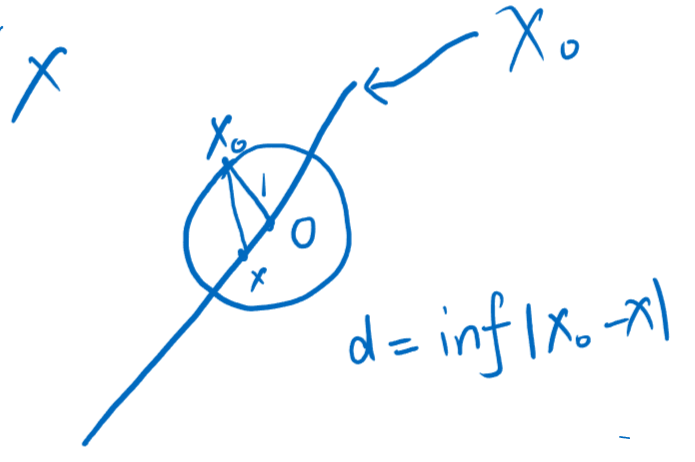
\includegraphics[scale=0.25]{./fig/3.5-1.png}
\end{figure}

对于$d(x_0,X_0)$我们首先应该能想到应该对应于$x_0 \perp X_0$,但是在赋范线性空间我们没办法定义垂直这件事,而$Riesz$引理告诉我们我们能找到一个差不多垂直的元素,当然由于差不多垂直,所以并不能保证$d(x_0,X_0) \geq 1$成立。
但是如果我们在有限维空间中考虑这件事,由完备性可知确实一定存在一个点满足$d(x_0,X_0) \geq 1$,\textbf{所以还是有限维香啊}。
我们可以严格描述并证明上面这句话。

\begin{proposition}
    若$X_0$为有限维真闭子空间,则$\exists \, x_0 \in S \quad \text{s.t.} \quad d(x_0,X_0)=1$。
\end{proposition}
\textbf{Proof:} 
\[\forall y_0 \in X/X_0 \ , \ d:=d(y_0,X_0)>0 \ , \ \exists \, x_0 \in X_0 \quad \text{s.t.} \quad d \leq d(t_0,x_n)<d(y_0,x_0)-\frac{1}{n}\]
通过上述方式构造出的点列$\{x_n\}$满足$||x_n|| \leq ||x_n-y_0||+||y_0||<+\infty$,是有限维闭子空间上的点列,由有限维赋范线性空间的性质可知$\{x_n\}$列紧,不妨设$x_n \to x_0 \in X_0$,其中$x_0$被称为\textbf{最佳逼近元}。
\[d \leq d(y_0,x_n)<d(y_0,x_0)-\frac{1}{n} \ (n \to \+\infty) \quad \Rightarrow \quad d(y_0,x_0)=d\]
取球面上另外一点$x'$满足如下条件可验证$d(x',X_0)=1$。
\[x'=\frac{y_0-x_0}{||y_0-x_0||} \quad \Rightarrow \quad d(x',X_0)=\mathop \text{inf}\limits_{z \in X_0}\left\|\frac{y_0-x_0}{||y_0-x_0||}-z\right\|=\frac{1}{||y_0-x_0||}\mathop \text{inf}\limits_{z \in X_0}\left\|||y_0-x_0||z+x_0-y_0\right\|=\frac{1}{d} \cdot d=1\]

\textbf{Q.E.D.}

顺便严格定义一下最佳逼近元。
\begin{definition}[最佳逼近元]
    设$(X,||\cdot||)$是赋范线性空间,$Y$是$X$的子空间,对$x \in X$,如果
    \[\exists \, y_0 \in Y \quad \text{s.t.} \quad ||x-y_0||=d(x,Y)=\mathop \text{inf}\limits_{y \, \in Y}||x-y||\]
    则称$y_0$为$Y$上关于$X$的最佳逼近元。
\end{definition}

但是在一般的情形下(无限维),最佳逼近元可能不存在,我们可以看下面一个例子。

\paragraph*{例1} \quad 设$X=\left\{f \in C[0,1]|f(0)=0\right\}$,其中$X_0 \in X$为
\[X_0=\left\{f \in X \Big{|} \int_0^1f(x)\dd x=0\right\}\]
则不存在$f \in S \quad \text{s.t.} \quad d(f,X_0)=1$。\\
\textbf{Proof:} \quad 采用反证法,假设$\exists \, f \in S \quad \text{s.t.} \quad d(f,X_0)=1$。
\[f_0 \in X \quad \Rightarrow \quad f_0 \in C[0,1] \ , \ f_0(0)=0 \ , \ ||f_0||=\mathop \text{sup}\limits_{x \in [0,1]}|f(x)|=1 \quad \Rightarrow \quad \left|\int_0^1f_0(x)\dd x\right|<1\]
另一方面
\[\forall f \in X/X_0 \ , \ \exists \, a \in \mathbb{R}^1 \quad \text{s.t.} \quad \int_0^1(f_0-af)\dd x=0 \quad (a=\int_0^1f_0(x)\dd x \Big{/} \int_0^1f(x)\dd x)\]
即$f_0-af \in X_0$,则
\[||f_0-(f_0-af)||=|a|||f|| \geq d(f_0,X_0)=1 \quad \Rightarrow \quad \left|\int_0^1f_0(x)\dd x\right|||f|| \geq \left|\int_0^1f(x)\dd x\right|\]
特别的,我们可以取$f$为一族函数$f_n(x)=x^{1/n}$,则
\[||f_n||=1 \ , \ \left|\int_0^1f_n(x)\dd x\right|=\frac{n}{n+1}\]
进而
\[\left|\int_0^1f_0(x)\dd x\right|||f_n|| \geq \left|\int_0^1f_n(x)\dd x\right|=\frac{n}{n+1} \to 1 \quad (n \to +\infty)\]
得出矛盾。\\
\textbf{Q.E.D.}

同时,即使最佳逼近元存在也可能不唯一,再看一个例子。

\paragraph*{例2} \quad $X=\mathbb{R^2} \ , \ ||\mathbf{x}||=||(x_1,x_2)||=\text{max}\left\{|x_1|,|x_2|\right\}$,取$\mathbf{x}_0=(0,1) \ , \ \mathbf{e}_1=(1,0) \ , \ X_0=\text{span}\{\mathbf{e}_1\}$,
\[\forall \mathbf{y} \in X_0 \ , \ \mathbf{y}=\lambda \mathbf{e}_1=(\lambda,0) \ , \ ||\mathbf{x}_0-\mathbf{y}||\text{max}\left\{|\lambda|,1\right\} \geq 1\]
则可知$\forall ||\mathbf{y}|| \leq 1$都是最佳逼近元。

下面我们就可以开始证明之前提到过的判定赋范线性空间有限维的定理了。

\begin{theorem}
    赋范线性空间$X$为有限维当且仅当$X$中任意有界集都是列紧的。
\end{theorem}
\textbf{Proof:} 一方面,由于$X$与$\mathbb{R}^n$同胚,在$X$上的有界集$E$的像集$T(E)$在$\mathbb{R}^n$有界,而$\mathbb{R}^n$上的有界集$T(E)$列紧,再由同胚可知$X$上的有界集$E$列紧。

另一方面,采用反证法,假设$X$是无穷维,任取$e_1 \in S=\{x \in X | \, ||x||=1\}$,由$Riesz$引理
\[X_1=\text{span}\{e_1\} \ , \ \exists \, e_2 \in S \ , \ d(e_2,X_1)>1-\frac{1}{2}=\frac{1}{2}\]
进而
\[X_2=\text{span}\{e_1,e_2\} \ , \ e_3 \in S \ , \ d(e_3,X_2)>\frac{1}{2} \quad \Rightarrow \quad d(e_3,e_1)>\frac{1}{2} \ , \ d(e_3,e_2)>\frac{1}{2}\]
由反证条件,上述操作可以一直做下去,可以得到序列$\{e_n\} \subset X$满足
\[\forall i,j \in \mathbb{N} \ , \ d(e_i,e_j)>\frac{1}{2} \ , \ ||e_i||=1\]
由于$X$中任意有界集都是列紧的可知$\exists \, \{e_{n_k}\} \subset \{e_i\}$收敛,故矛盾。

\textbf{Q.E.D.}
\chapter{有界线性算子}
\begin{introduction}
    \item 有界线性算子~\ref{BX}
    \item $Banach$-$Steinhaus$定理~\ref{BS}
    \item 开映射定理与闭图像定理~\ref{kb}
\end{introduction}
\section{有界线性算子}\label{BX}
在正式介绍赋范线性空间的有界线性算子之前,我们可以回忆一下有限维的情形,设$X,Y$为有限维空间,根据上一小节的描述,我们不妨假设$X=\mathbb{R}^m,Y=\mathbb{R}^n$,考虑线性变换$L:\mathbb{R}^m \to \mathbb{R}^n$,选取基底$\{e_i\}_{i=1}^m \subset X , \{f_j\}_{j=1}^n \subset Y$,线性变换$L$在基底上有如下关系
\[Le_i=\sum_j^na_{ij}f_j \ (a_{ij} \in \mathbb{R})\]
则$L$等价于矩阵$A=(a_{ij})_{1 \leq i \leq m , 1 \leq j \leq n}$,取
\[x=\sum_{i=1}^m\xi_ie_i \in X \ , \ y=\sum_{j=1}^n\eta_jf_j \quad \text{则} \quad Lx=
\begin{pmatrix}
    a_{11} & a_{12} & \cdots & a_{1m} \\
    a_{21} & a_{22} & \cdots & a_{2m} \\
    \vdots & \vdots & \ddots & \vdots \\
    a_{n1} & a_{n2} & \cdots & a_{nm} \\
\end{pmatrix}
\begin{pmatrix}
    \xi_1 \\ \xi_2 \\ \vdots \\ \xi_m \\
\end{pmatrix}
=\begin{pmatrix}
    \eta_1 \\ \eta_2 \\ \vdots \\ \eta_n \\
\end{pmatrix}
=y
\]

众所周知,泛函分析至少无穷维的线性代数,所以类似的我们可以延拓线性变换的定义到线性算子。
\begin{definition}[线性算子]
    设$X,Y$是赋范线性空间,$T$是从$X$的线性子空间$D(T) \subset X$到$Y$的映射,若其满足
    \[\forall x,y \in X \ , \ \alpha,\beta \in \mathbb{K} \ , \ T(\alpha x+\beta y)=\alpha Tx+\beta Ty\]
\end{definition}
值得注意的是线性算子的定义并不要求其定义域是出发空间的全空间,只要求是出发空间的一个线性子空间即可,当然可以是平凡子空间$(D(T)=X)$,但是默认全空间更省事所以一般默认全空间,同时无穷维的子空间也可以是稠密的$(C[0,1] \subset L[0,1])$。

回应一下章节标题,现在该定义线性算子的有界。
\begin{definition}[有界线性算子]
    设$T:X \to Y$是线性算子,若其满足
    \[\exists \, M>0 \quad \text{s.t.} \quad ||Tx||_Y \leq M||x||_x \ (\forall x \in X)\]
    则称其为有界线性算子。
\end{definition}
从$X \to Y$的全体有界线性算子记为$\mathscr{B}(X,Y)$。有界线性算子具有一些不错的性质,可以看下面一个定理。
\begin{theorem}
    设$T:X \to Y$是线性算子,则:\\
    1、$T$连续等价于$T$在一点处连续;\\
    2、$T$连续等价于$T$有界。
\end{theorem}
\textbf{Proof} of (1):“$\Rightarrow$” 显然

“$\Leftarrow$” 设$T$在$x_0 \in X$连续$\quad \Leftrightarrow \quad x_n \to x \ \Rightarrow \ Tx_n \to Tx$,则有
\[Tx_n-Tx=T(x_n-x+y)-Ty \to 0 \quad (\forall y \in X)\]

\textbf{Proof} of (2):“$\Leftarrow$” 由(1)知只需证明在一点处连续,不妨取为原点,取收敛于原点的点列$\{x_n\}$,由有界性
\[||Tx_n|| \leq M||x_n|| \to 0 \quad \Rightarrow \quad Tx_n \to 0 \quad \Leftrightarrow \quad Tx_n-T0 \to 0 \ (x_n-0 \to 0)\]

“$\Rightarrow$” 反证,设$T$连续但是无界,$\forall n \in \mathbb{N} \ , \ \exists \, x_n \in X \quad \text{s.t.} \quad ||Tx_n||>n||x_n||$,令
\[y_n=\frac{x_n}{n||x_n||} \ , \ ||y_n||=\frac{||x_n||}{n||x_n||}=\frac{1}{n} \to 0 \quad \Rightarrow \quad y_n \to 0\]

由线性性可知$T0=0$,而
\[||Ty_n-T0||=||Ty_n||=\left\|\frac{Tx_n}{n||x_n||}\right\|>1\]

与连续性矛盾。

\textbf{Q.E.D.}

上面提到了算子的有界性,那么自然外面会想用一个指标来衡量一个算子到底多有界,于是就有了算子范数的概念。
\begin{definition}[算子范数]
    设$T \in \mathscr{B}(X,Y)$,定义算子范数
    \[||T||=\mathop \text{sup}\limits_{x \in X/\{0\}}\frac{||Tx||}{||x||}=\mathop \text{sup}\limits_{||x||=1}||Tx||=\mathop \text{sup}\limits_{||x|| \leq 1}||Tx||\]
\end{definition}
既然叫范数说明$||T||$满足范数要求的条件这里不过多赘述,同时上述三个定义也是等价的,这些内容留待读者自证(笑

因此$(\mathscr{B}(X,Y),||\cdot||)$就构成了一个赋范线性空间,这还是比较有意思的,当然后面会更有意思(笑

另外一件事关于之前提到的线性算子的定义域的内容,我们说线性算子的定义域可以是出发空间的一个子空间也可以是出发空间本身,这两者在叫法上就区分为:
1、$T:D(T)=X \to Y$在$X$上到$Y$上;2、$T:D(T) \subset X \to Y$在$X$中到$Y$上。

下面我们来看几个例子。
\paragraph*{例1} \quad $X=\mathbb{R}^m,Y=\mathbb{R}^n \ , \ L \in \mathscr{B}(X,Y)$,选定基底后$L$等价于矩阵$A=(a_{ij})_{m \times n}$,分别取$X,Y$空间中的两个元素,$x,y$满足
\[x=(\xi_1,\xi_2,\cdots,\xi_m)^{\text{T}} \ , \ y=(\eta_1,\eta_2,\cdots,\eta_n)^{\text{T}} \ , \ Lx=y\]
则
\[||Lx||=||y||=\sqrt{\sum_{i=1}^n|\eta_i|^2}=\sqrt{\sum_{i=1}^n\left|\sum_{j=1}^ma_{ij}\xi_j\right|^2} \leq \sqrt{\sum_{i=1}^n\sum_{j=1}^ma_{ij}^2 \cdot \sum_{j=1}^m\xi_j^2}=\text{tr}(A^{\text{T}}A)^{\frac{1}{2}}||x||:=||A||\cdot||X||\]
由上确界性质可知$||L|| \leq ||A||$,实际上是取等。

\paragraph*{例2} \quad 微分算子,一维情形下,考虑$X=C[0,1] \ , \ T:X \to X \ , \ x(t) \mapsto Tx=x'(t)$,则该算子为无解算子:
\[x_n(t)=\sin nt \ , \ ||x_n||=1 \quad \Rightarrow \quad Tx_n=x_n'(t)=n \cos nt \ , \ ||Tx_n||=n \to +\infty\]

高维情形下也类似,考虑$\Omega \subset \mathbb{R}^n$,记$C^k(\bar{\Omega})=\{f:\bar{\Omega} \to \mathbb{R}|\partial^{\alpha}f \in C(\bar{\Omega}) \ , \ |\alpha| \leq k\}$,其上范数为:
\[||f||_{C^k}=\mathop \text{max}\limits_{|\alpha| \leq k}||\partial^{\alpha}f||_{C^0}=\mathop \text{max}\limits_{|\alpha| \leq k}\mathop \text{max}\limits_{x \in \bar{\Omega}}|\partial^{\alpha}f(x)|\]
其中
\[\alpha=(\alpha_1,\alpha_2,\cdots,\alpha_n) \ , \ \partial^{\alpha}f=\partial^{\alpha_1}_{x_1}\partial^{\alpha_2}_{x_2}\cdots\partial^{\alpha_n}_{x_n}f(x_1,x_2,\cdots,x_n) \ , \ \sum_{i=1}^n\alpha_i \leq k\]
因此,在高维版本中上述的一维微分算子可表示为
\[X=C^{\infty}(\bar{\Omega})=\bigcap_{k=1}^{\infty}C^k(\bar{\Omega}) \ , \ T:X \to X \ , \ x(t) \mapsto Tx=\sum_{|\alpha| \leq k}a_{\alpha}(t)\cdot\partial^{\alpha}x(t)\]
其依然是无界算子,反例类似一维。

\paragraph*{例3} \quad 积分算子,考虑 $L^2$上的$Lebesgue$积分
\[X=L^2(\bar{\Omega}) \ , \ T:X \to \mathbb{R}^n \ , \ u(x) \mapsto Tu=\int_{\bar{\Omega}}u(x)\psi(x)\dd x\]
由柯西不等式
\[||Tu||=|Tu| \leq ||u||_{L^2}||\psi||_{L^2} \quad \Rightarrow \quad ||T|| \leq ||\psi||_{L^2}\]
再由
\[||T\psi||=|T\psi|=\int_{\bar{\Omega}}|\psi|^2=||\psi||_{L^2}^2 \quad \Rightarrow \quad ||T||=||\psi||_{L^2}\]

\section{有界线性算子空间}
上一小节中,我们提及有界线性算子全体构成一个赋范线性空间$(\mathscr{B}(X,Y),||\cdot||)$,自然而然我们也会想知道在这样一个赋范线性空间上,元素的收敛性该如何刻画,这对后面讨论空间完备性时至关重要。
\begin{theorem}
    点列$\{T_n\} \subset \mathscr{B}(X,Y)$依范数收敛于$T$当且仅当$\{T_n\}$在单位球面$S=\{x \in X| \, ||x||=1\}$一致收敛于$T$。
\end{theorem} 
在证明之前,先明确算子空间中的这两种收敛方式,依范数收敛指$||T_n-T|| \to 0$;一致收敛指的是$\forall \varepsilon>0 \ , \ x \in S \ , \ \exists \, N(\varepsilon) \in \mathbb{N} \quad \text{s.t.} \quad n>N \ , \ ||T_n(x)-T(x)||<\varepsilon$。
与一般赋范线性空间中的同名定义保持一致。

\textbf{Proof}:
\[||T_n-T|| \to 0 \quad \Rightarrow \quad \forall x \in S \ , \ ||T_n(x)-T(x)|| \leq \mathop \text{sup}\limits_{x \in S}||(T_n-T)x||=||T_n-T||<\varepsilon\]
\[\forall x \in S \ , \ \exists \, N \in \mathbb{N} \quad \text{s.t.} \quad n>N \ , \ ||T_n(x)-T(x)||<\varepsilon \quad \Rightarrow \quad ||T_n-T||=\mathop \text{sup}\limits_{x \in S}||(T_n-T)x||<\varepsilon\]

\textbf{Q.E.D.}

虽然这个定理一眼顶针鉴定为放屁,但既然上课讲了那我还是放进来了。

下面这个定理就没那么显然了,如果我们想知道一个算子空间完备需要什么条件,那么按照定义自然而然地就需要其上的所有柯西列都收敛于其中。
我们可能会猜想这需要出发空间和到达空间都完备,但如果考虑算子范数的定义,好像跟出发空间没什么太大关系,于是我们进一步猜测只跟到达空间有关系。
那么到底是不是呢,答案是yes,下面我们来叙述这件事并证明它。
\begin{theorem}
    如果$Y$是$Banach$空间,则$\mathscr{B}(X,Y)$也是$Banach$空间。
\end{theorem} 
\textbf{Proof}:设$\{T_n\}$为$\mathscr{B}(X,Y)$中的柯西列,则有
\[\forall \varepsilon>0 \ , \ \exists \, N \in \mathbb{N} \quad \text{s.t.} \quad \forall n>N \ , \ p \in \mathbb{N} \ , \ ||T_{n+p}-T_n||<\varepsilon\]
则
\[\forall x \in X \ , \ ||T_{n+p}(x)-T_n(x)|| \leq ||T_{n+p}-T_n|| \cdot ||x||<\varepsilon||x||\]
即$\{T_n(x)\}$是$Y$中的柯西列,由完备性知其收敛,设$\forall x \in X \ , \ T_n(x) \to T(x)$,则只需验证$T \in \mathscr{B}(X,Y)$即可:\\
1、线性
\[T(\alpha x+\beta y)=\lim_{n \to +\infty}T_n(\alpha x+\beta y)=\alpha\lim_{n \to +\infty}T_nx+\beta\lim_{n \to +\infty}T_ny=\alpha Tx+\beta Ty\]
2、有界性
\[\forall x \in X \ , \ ||Tx||=\left\|\lim_{n \to +\infty}T_nx\right\|=\lim_{n \to +\infty}||T_nx||<+\infty \quad \Rightarrow \quad ||Tx|| \leq M||x||\]
\[||Tx|| \leq ||Tx-T_nx||+||T_nx|| \leq (\varepsilon+M)||X|| \quad \Rightarrow \quad ||T||<\varepsilon+M\]

\textbf{Q.E.D.}

上面提到了算子空间中的依范数收敛和一致收敛,下面我们也把逐点收敛定义一下。
\begin{definition}[(算子空间的)逐点收敛]
    设$T_n,T \in \mathscr{B}(X,Y)$,若$\forall x \in X \ , \ T_nx \to Tx$则称,$T_n$强收敛(逐点收敛)于$T$,即
    \[\forall x \in X \ , \ \varepsilon>0 \ , \ \exists \, N(\varepsilon,x) \in \mathbb{N} \quad \text{s.t.} \quad \forall n>N \ , \ ||T_nx-Tx||<\varepsilon\]
\end{definition}
显然,依范数收敛可以推出逐点收敛。下面我们来看个例子:
\paragraph*{例} \quad $X=l^p \ , \ \forall x=(\xi_1,\xi_2,\cdots,\xi_n,\cdots) \ , \ T_nx:=(\xi_{n+1},\xi_{n+2},\cdots)$,则
\[\forall x \in l^p \ , \ ||T_nx||=\left(\sum_{k=n}^{+\infty}|\xi_k|^p\right)^{\frac{1}{p}} \to 0\]
$\Rightarrow \quad T_n$逐点收敛于$0$。\\
但是$T_n$不依范数收敛于$0$,考虑$x_k=(0,0,\cdots,0,1,0,\cdots) \in S$ ($1$在第$k$位),则$||T_n(x_n)||=(1,0,\cdots) \leq ||T_n||$。

\section{$Banach$-$Steinhaus$定理}
冲本小结开始,我们将逐步介绍泛函中的几个最重要的定理,上一小节中我们初步讨论了算子空间中的收敛性问题,但是在收敛之前,我们也许可能大约应该先看看有界性。
一般的赋范线性空间中我们已经定义了逐点有界和一致有界,在算子空间中我们同样也能定义这两者,考虑算子空间中的一族算子$\{T_{\alpha}\}_{\alpha \in \Lambda} \subset \mathscr{B}(X,Y)$:

若称$\{T_{\alpha}\}$一致有界,即$\forall x \in X \ , \ \exists \, M>0 \quad \text{s.t.} \quad ||T_{\alpha}x|| \leq M||x|| \quad \Rightarrow \quad \exists \, M>0 \quad \text{s.t.} \quad ||T_{\alpha}|| \leq M$;

若称$\{T_{\alpha}\}$逐点有界,即$\forall x \in X \ , \ \exists \, M(x)>0 \quad \text{s.t.} \quad ||T_{\alpha}x|| \leq M(x)||x||$ or $M(x)$。

显然,在算子空间中一致有界还是强于逐点有界,那么我们自然会思考在什么条件下逐点有界能反推出一致有界,这就是$Banach$-$Steinhaus$定理所回答的问题。
\begin{theorem}[一致有界定理]
    $\{T_{\alpha}\}_{\alpha \in \Lambda} \subset \mathscr{B}(X,Y) \ , \ D(T_{\alpha})=X$ ,若$X$是$Banach$空间,则$\{T_{\alpha}\}$一致有界当且仅当$\{T_{\alpha}\}$逐点有界。
\end{theorem} 
\textbf{Proof}:证明分为两步,先证在某个开集(开球)上成立($Baire$纲定理),再证在全空间上成立(利用线性)。从一致有界到逐点有界显然,下证逐点有界到一致有界。定义映射
\[p:X \to \mathbb{R} \ , \ p(x)=\mathop \text{sup}\limits_{\alpha \in \Lambda}||T_{\alpha}x|| \quad \Rightarrow \quad \forall x \in X \ , \ \quad p(x)<+\infty\]
定义化分集合
\[M_k=\{x \in X|p(x) \leq k\}=\bigcup_{\alpha \in \Lambda}\{x \in X| \, ||T_{\alpha}x|| \leq k\} \quad (k \in \mathbb{N})\]
则
\[X=\bigcap_{k=1}^{\infty}M_k\]
由$Baire$纲定理,$X$是$Banach$空间,为第二纲集,从而存在$k_0 \in \mathbb{N}$使得$M_{k_0}$不是疏集,即
\[\exists \, B_r(x_0)=\{x \in X| \, ||x-x_0||<r\} \quad \text{s.t.} \quad B_r(x_0) \subset \overline{M}_k\]
由$T_{\alpha}$的连续性可知,$[0,k]$的原像$\{x \in X| \, ||T_{\alpha}x|| \leq k\}$是闭集,从而$M_k$也是闭集
\[B_r(x_0) \subset \overline{M}_k=M_k \quad \Leftrightarrow \quad \forall x \in B_r(x_0) \ , \ p(x)=\mathop \text{sup}\limits_{\alpha \in \Lambda}||T_{\alpha}x|| \leq k\]
第一步即证,利用线性可以将该结论推广至全空间
\[\forall y \in X \ , \ \alpha \in \Lambda \ , \ \exists \, M=\frac{2k}{r} \quad \text{s.t.} \quad ||T_{\alpha}y||=\left\|T_{\alpha}\left(x_0+\frac{r}{||y||}y\right)-T_{\alpha}x_0\right\| \cdot \frac{||y||}{r} \leq \frac{||y||}{r}(k+k)=M||y||\]

\textbf{Q.E.D.}

从上面的证明来看,一致有界定理可以扩展到出发空间是第二纲集,其逆否定理叫共鸣定理。
\begin{theorem}[共鸣定理]
    $\{T_{\alpha}\}_{\alpha \in \Lambda} \subset \mathscr{B}(X,Y) \ , \ D(T_{\alpha})=X$ , $X$是$Banach$空间,若$||T_{\alpha}||=+\infty$则,$\exists \, x \in X \quad \text{s.t.} \quad ||T_{\alpha}x||=+\infty$。
\end{theorem} 
相比于一般的常见赋范线性空间,算子空间的性质不是那么任意直观看出,如果能利用出发空间和到达空间的性质判断算子空间的性质自然是最好的。
为了回答这个问题,结合上一小节的收敛性和这一小节的有界性,我们介绍$Banach$-$Steinhaus$定理。
\begin{theorem}[$Banach$-$Steinhaus$定理]\label{BS}
    $\{T_n\}_{n=1}^{+\infty} \subset \mathscr{B}(X,Y) \ , \ D(T_{\alpha})=X$ ,若$Y$是$Banach$空间,若:\\
    1、$\{T_n\}$一致有界;\\
    2、$\{T_n\}$在$X$的一个稠密$G$上逐点收敛($\forall g \in G \ , \ \{T_ng\}$收敛);\\
    则,$\exists \, T \in \mathscr{B}(X,Y) \quad \text{s.t.} \quad \{T_n\}$逐点收敛于$T$,且
    \[||T|| \leq \varliminf\limits_{n\to\infty}||T_n||\]
\end{theorem} 
\textbf{Proof}:由于$G$在$X$上稠密,即$\forall x \in X \ , \ \varepsilon>0\ , \ \exists \, g \in G \quad \text{s.t.} \quad ||x-g||<\varepsilon$,$\exists \, N \in \mathbb{N} \quad \text{s.t.} \quad \forall m>n>N$
\[||T_mx-T_nx|| \leq ||T_mx-T_mg||+||T_mg-T_ng||+||T_ng-T_nx|| \leq \left(||T_m||+||T_n||\right)||x-g||+\varepsilon \leq (2M+1)\varepsilon\]
即$\{T_nx\}$是$Y$空间中的$Cauchy$列,由$Y$空间完备
\[\exists \, y \in Y \quad \text{s.t.} \quad \lim_{n \to \infty}T_nx=y:=Tx\]
下面只需验证$T$为有界线性算子:\\
1、线性
\[T(\alpha x+\beta y)=\lim_{n \to +\infty}T_n(\alpha x+\beta y)=\alpha\lim_{n \to +\infty}T_nx+\beta\lim_{n \to +\infty}T_ny=\alpha Tx+\beta Ty\]
2、有界性
\[||Tx||=\left\|\lim_{n \to +\infty}T_nx\right\|=\varliminf\limits_{n\to\infty}||T_nx|| \leq \varliminf\limits_{n\to\infty}||T_n|| \cdot ||x|| \quad \Rightarrow \quad ||T|| \leq \varliminf\limits_{n\to\infty}||T_n||\]

\textbf{Q.E.D.}

$Banach$-$Steinhaus$定理告诉我们利用完备到达空间的收敛怎么样推出算子空间的收敛,这无疑是一种极大的方便。
同时,该定理也说明了$\mathscr{B}(X,Y)$在强收敛意义下完备。下面看几个例子。

\paragraph*{例1(机械求积分公式)} \quad 令$X=C[a,b] \ , \ \forall x \in X$有
\[\int_a^bx(t)\dd t \approx \sum_{k=1}^nA_kx(t_k) \quad (a \leq t_1<t_2<\cdots<t_k\leq b\text{是}[a,b]\text{的分割})\]
则下式
\[\int_a^bx(t)\dd t=\lim_{n \to \infty}\sum_{k=1}^nA_k^{(n)}x(t_k^{(n)}) \quad (\text{其中}A_k^{(n)}\text{只与参数}n\text{有关而与}x(t)\text{无关}) \tag{*}\]
成立的充要条件为
\[\mathbf{1.} \ \forall n \in \mathbb{N} \ , \ \exists \, M>0 \quad \text{s.t.} \quad \sum_{k=1}^n\left|A_k^{(n)}\right| \leq M \qquad \mathbf{2.} \ (*)\text{式对} \, C[a,b] \, \text{的一个稠密子集} \, G \, \text{成立}\]
\textbf{Proof}:构造一列$X=C[a,b]$上的泛函$\{f_n\}$:
\[f_n:X \to \mathbb{R} \ , \ f_n(x)=\sum_{k=1}^nA_k^{(n)}x(t_k^{(n)})\]

为了保证$\{f_n\}$强收敛于原积分,必须保证其线性,至此我们只需要验证
\[||f_n||=\sum_{k=1}^n\left|A_k^{(n)}\right|\]
即可利用$Banach$-$Steinhaus$定理证明原命题。\\
一方面
\[\forall x \in X \ , \ ||f_n(x)||=\left|\sum_{k=1}^nA_k^{(n)}x(t_k^{(n)})\right| \leq ||x||\sum_{k=1}^n\left|A_k^{(n)}\right| \quad \Rightarrow \quad ||f_n|| \leq \sum_{k=1}^n\left|A_k^{(n)}\right|\]
另一方面
\[\exists \, x_0 \in X \ , \ s_0(t_k^{(n)})=\text{sgn}(A_k^{(n)}) \quad \Rightarrow \quad ||x_0||=1 \ , \ ||f_n(x_0)||=\left|\sum_{k=1}^nA_k^{(n)}\text{sgn}(A_k^{(n)})\right|=\sum_{k=1}^n\left|A_k^{(n)}\right| \leq ||f_n||\]
综上所述
\[||f_n||=\sum_{k=1}^n\left|A_k^{(n)}\right|\]

\textbf{Q.E.D.}

\paragraph*{例2($Fourier$级数的发散性)} \quad 考虑
\[X=C_{2\pi}=\{x \in C[0,2\pi]|x(0)=x(2\pi)\}=\{x \in C(\mathbb{R})|x(t+2\pi)=x(t) \ , \ \forall t \in \mathbb{R}\}\]
$\forall x \in X$,考察$Fourier$级数
\[x(t) \sim \frac{a_0}{2}+\sum_{i=1}^{+\infty}(a_k \cos kt+b_k \sin kt):=\lim_{n \to \infty}F_nx(t)\]
其中c
\[a_k=\frac{1}{\pi}\int_{-\pi}^{\pi}x(s) \cos ks \dd s \ , \ b_k=\frac{1}{\pi}\int_{-\pi}^{\pi}x(s) \sin ks \dd s\]

这里回顾一下$Dirichlet$条件,他只是判断$Fourier$级数收敛的一个充分条件。
\begin{theorem}[$Dirichlet$条件]
    若$x \in C_{2\pi}$在$[0,2\pi]$上满足:1、之多有限个第一类间断点;2、至多有限个极值点,则
    \[\lim_{n \to \infty}F_nx(t)=\left\{
        \begin{array}{rl}
            x(t) & ,x\text{在}t\text{处连续} \\
            \frac{1}{2}(x(t^-)+x(t^+)) & ,t\text{是}x\text{的第一类间断点}
        \end{array}
    \right.\]
\end{theorem} 
下面我们将利用共鸣定理说明不加条件时,$Fourier$级数可能不收敛。定义
\[f_n:X \to \mathbb{R} \ , \ x(t) \mapsto f_nx(0)=\int_{-\pi}^{\pi}x(s)k_n(s,0) \dd s \quad \text{其中 }k_n(s,t)=\frac{1}{\pi}\left(\frac{1}{2}+\sum_{k=1}^n\cos k(s-t)\right)\]
可以证明如下两个事实
\[\mathbf{1.} \ ||f_n||=\int_{-\pi}^{\pi}|k_n(s,0)| \dd s \qquad \mathbf{2.} \ ||f_n|| \to 0\]
然后由共鸣定理可知
\[\exists \, x \in X \quad \text{s.t.} \quad |f_nx(0)| \to +\infty\]

\section{开映射定理与闭图像定理}\label{kb}
在介绍标题的两个定理之前,我们需要补充一下算子的复合和逆算子的概念。
\begin{definition}[算子复合(乘法)]
    设$X,X_1,X_2$是赋范线性空间,$T_1:X \to X_1$,$T_2:X_1 \to X_2$,$R(T_1) \subset D(T_2)$,定义算子复合$T=T_2 \circ T_1=T_2T_1$,
    \[\forall x \in X \ , \ Tx=(T_2 \circ T_1)x=T_2(T_1x)\]
\end{definition}
若$T_1 \in \mathscr{B}(X,X_1) \ , \ T_2 \in \mathscr{B}(X_1,X_2)$,则$T \in \mathscr{B}(X,X_2)$。
\[||Tx||=||T_2(T_1x)|| \leq ||T_2||\cdot||T_1||\cdot||x|| \quad \Rightarrow \quad ||T|| \leq ||T_1||\cdot||T_2||\]
另一方面,这也说明了连续算子的复合得到的还是连续算子。

下面我们可以定义逆算子:
\begin{definition}[逆算子]
    设$X,Y$是赋范线性空间,$T_1:X \to Y$,若$\exists \, T_1:Y \to X \quad \text{s.t.} \quad T_1 \circ T=I_X \ , \ T \circ T_1=I_Y$,则称$T$可逆,$T_1$是$T$的逆算子,记$T_1=T^{-1}$。
\end{definition}
逆算子有一些显然的性质,比如$T$是线性的则$T^{-1}$也是线性的;算子$T$可逆当且仅当$T$是一一映射;若$T^{-1}$存在则唯一等等。

那么我们会思考如果$T$是有界线性算子,$T^{-1}$是否也是有界,或者说$T^{-1}$是否连续呢?这件事开映射定理及逆算子定理会告诉我们。但是在正式介绍这两个定理之前我们可以从一些比较具体的情况开始逐步推广。
\begin{theorem}
    设$T \in \mathscr{B}(X)$是满射,且$\forall x \in X \ , \ \exists \, m>0 \quad \text{s.t.} \quad ||Tx|| \geq m||x||$,则$T$可逆且$T^{-1} \in \mathscr{B}(x)$。
\end{theorem} 
\textbf{Proof}:\\
$T$是单射:
\[\forall x_1,x_2 \in X \ , \ ||Tx_1-Tx_2|| \geq m||x_1-x_2|| \ , \ ||Tx_1-Tx_2||=0 \quad \Leftrightarrow \quad ||x_1-x_2||=0\]
$T^{-1}$有界:
\[\forall y \in X \ , \ ||T^{-1}Y||:=||x|| \leq m||Tx||=m||y||\]

\textbf{Q.E.D.} 
\begin{theorem}
    设$X$是$Banach$空间,$T \in \mathscr{B}(X) \ , \ ||T||<1$,则算子$I-T$可逆,且
    \[||(I-T)^{-1}|| \leq \frac{1}{1-||T||}\]
\end{theorem} 
\textbf{Proof}:设
\[S_n=\sum_{k=0}^{n-1}T^k \ , \ T^0:=I\]
\[\forall m>n \ , \ ||S_m-S_n||=\left\|\sum_{k=n}^{m-1}T^k\right\| \leq \sum_{k=n}^{m-1}||T^k|| \leq \sum_{k=n}^{m-1}||T||^k=||T||^n \cdot \frac{1-||T||^{m-n}}{1-||T||}<\frac{||T||^n}{1-||T||} \to 0\]
可知$\{S_n\}$是柯西列,由于$X$是$Banach$空间,故$\{S_n\}$收敛,记其收敛极限为
\[S:=\sum_{k=0}^{+\infty}T^k\]
为了证明$S$是$I-T$的逆,我们考虑
\[S_n \circ (I-T)=(I-T) \circ S_n=I-T^n\]
\[(I-T) \circ S=S \circ (I-T)=\lim_{n \to +\infty}S_n \circ (I-T)=\lim_{n \to +\infty}(I-T^n)\]
注意到
\[\lim_{n \to +\infty}||T^n|| \leq \lim_{n \to +\infty}||T||^n=0 \quad \Rightarrow \quad \lim_{n \to +\infty}T^n=\mathbf{0} \ (\text{零算子})\]
故
\[(I-T) \circ S=S \circ (I-T)=I \quad \Rightarrow \quad S=(I-T)^{-1}\]
\[||(I-T)^{-1}||=||S||=\left\|\lim_{n \to +\infty}S_n\right\|=\left\|\lim_{n \to +\infty}\sum_{k=0}^{n-1}T^k\right\| \leq \lim_{n \to +\infty}\sum_{k=0}^{n-1}||T||^k=\lim_{n \to +\infty}\frac{1-||T||^n}{1-||T||}=\frac{1}{1-||T||}\]

\textbf{Q.E.D.}

上述定理向我们展示了恒同算子加上一个小的扰动($||T||<1$)时依然可逆,那我们自然会考虑这件事是否对任意可逆算子成立。
\begin{theorem}
    设$X$是$Banach$空间,$T \in \mathscr{B}(X)$,$T^{-1} \in \mathscr{B}(X)$可逆,若
    \[\Delta T \in \mathscr{B}(X) \ , \ ||\Delta T||<\frac{1}{||T^{-1}||} \ , \ S:=T+\Delta T \in \mathscr{B}(X) \ \text{可逆且} \ S^{-1}=\sum_{k=0}^{+\infty}(-1)^k(T^{-1}\Delta T)^kT^{-1}\]
\end{theorem} 
\textbf{Proof}:设
\[S=T+\Delta T=T \circ (I+T^{-1}\Delta T) \ , \ ||T^{-1}\Delta T|| \leq ||T^{-1}|| \cdot ||\Delta T||<1\]
由上一定理知$I+T^{-1}\Delta T$可逆,且
\[(I+T^{-1}\Delta T)^{-1}=\sum_{k=0}^{+\infty}(-T^{-1}\Delta T)^k \quad \Rightarrow \quad S^{-1}=\sum_{k=0}^{+\infty}(-1)^k(T^{-1}\Delta T)^kT^{-1}\]
\textbf{Q.E.D.}

上述定理中提及的$T,T^{-1} \in \mathscr{B}(X)$的这类算子称为正则算子,$Banach$空间到$Banach$空间的正则算子构成的集合为开集。

经过上述铺垫我们现在可以介绍开映射定理了。
\begin{theorem}[开映射定理]
    设$X,X_1$是$Banach$空间,$T \in \mathscr{B}(X,X_1) \ , \ TX=X_1$,则$T$是开映射。
\end{theorem} 
在证明该定理前,我们需要先介绍一下开映射以及考虑一下是否能简化证明流程。开映射顾名思义是指将开集映为开集,即$\forall y \in TX \ , \ \exists \, \delta>0 \quad \text{s.t.} \quad B_1(y,\delta) \subset TU$,由线性可知只需要对零点证明该定理即可。
\[\forall y=Tx \in TU \ , \ \exists \, \varepsilon>0 \ \text{s.t.} \ B(x,\varepsilon) \subset U \ \Rightarrow \ \exists \, \delta>0 \ , \ TB(x,\varepsilon)=T(x+\varepsilon B(0,1)) \supset Tx+B_1(0,\delta)=B_1(y,\delta)\]

\begin{figure}[H]
    \center
    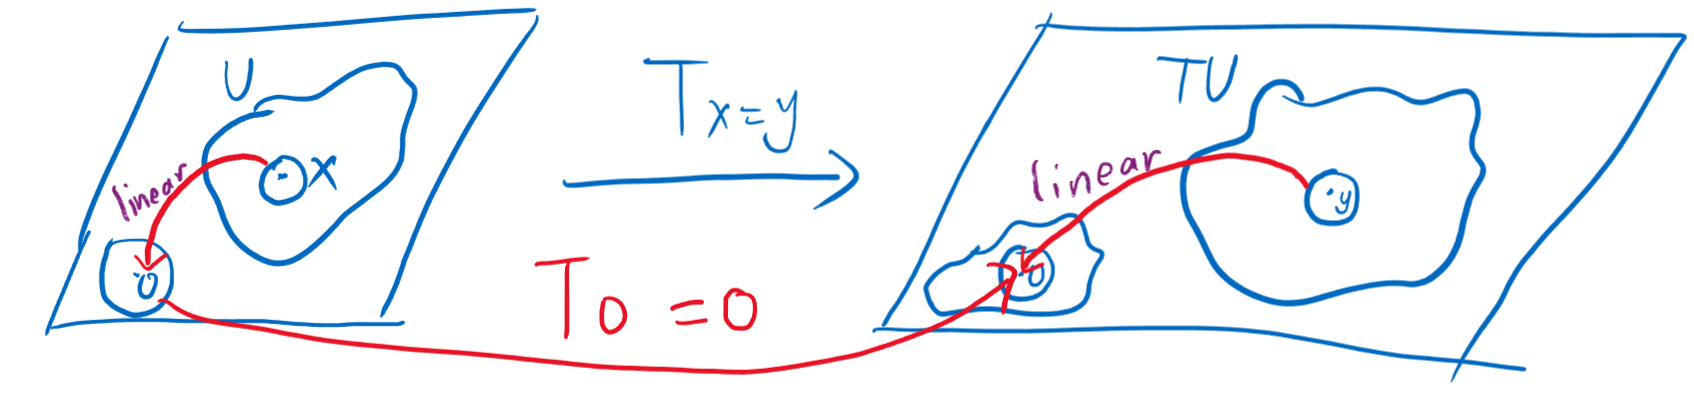
\includegraphics[scale=0.3]{./fig/4.4-1.png}
\end{figure}

\textbf{Proof}:分两步证明$T0$是$TB(0,1)$的内点。

\textbf{Step 1. }证明$T\overline{B(0,1)}$在某个$B_1(0,\delta)$中稠密。

由于$T$是满射,即$TX=X_1$,且$X_1$是全空间
\[X=\bigcup_{k=1}^{\infty}\overline{B(0,k)} \quad \Rightarrow \quad X_1 \subseteq \bigcup_{k=1}^{\infty}T\overline{B(0,k)} \quad \Rightarrow \quad X_1=\bigcup_{k=1}^{\infty}T\overline{B(0,k)}\]

由于$X_1$是$Banach$空间,为第二纲集,故存在某个开球$B_1(y_0,r_0) \subset T\overline{B(0,K_0)}$。
\[\forall y \in B_1(0,r_1) \ , \ y=\frac{1}{2}[(y_0+y)-(y_0-y)]:=\frac{1}{2}(y_1-y_2) \ , \ y_1,y_2 \in B_1(y_0,r_0)\]
\[\forall \varepsilon>0 \ , \ y_1,y_2 \in B_1(y_0,r_0) \ , \ \exists \, x_1,x_2 \in \overline{B(0,k_0)} \quad \text{s.t.} \quad ||Tx_1-y_1||<\varepsilon \ , \ ||Tx_2-y_2||<\varepsilon\]
\[\forall \varepsilon>0 \ , \ y=\frac{y_1-y_2}{2} \in B_1(0,r_1) \ , \ \exists \, x=\frac{x_1-x_2}{2} \in \overline{B(0,k_0)} \quad \text{s.t.} \quad ||Tx-y||=\left\|T\left(\frac{x_1-x_2}{2}\right)-\frac{1}{2}(y_1-y_2)\right\|<\varepsilon\]
即$T\overline{B(0,k_0)}$在$B_1(0,r_0)$中稠密,从而$\forall \varepsilon>0 \ , \ T\overline{B(0,\varepsilon)}$在$B_1(0,\delta\varepsilon)$中稠密,其中$\delta=r_0/k_0$,可取$\varepsilon=1$。

\textbf{Step 2. }证明$T\overline{B(0,1)} \supset B_1(0,\delta/2)$。

由$T\overline{B(0,1/2)}$在$B_1(0,\delta/2)$中稠密,可知
\[\forall y \in B_1(0,\frac{\delta}{2}) \ , \ \exists \, x_1 \in B(0,\frac{1}{2}) \quad \text{s.t.} \quad ||y-Tx_1||<\frac{\delta}{2^2} \quad \Leftrightarrow \quad y_1:=y-Tx_1 \in B_1(0,\frac{\delta}{2^2})\]
以此类推可得
\[\exists \, \{x_n\} \subset B(0,1) \ , \ ||x_n|| \leq \frac{1}{x^n} \ , \ \left\|y-T\left(\sum_{k=1}^nx_k\right)\right\|<\frac{\delta}{2^{n+1}}\]
\[S_n:=\sum_{k=1}^nx_k \ , \ m>n>N \ , \ ||S_m-S_n||=\left\|\sum_{k=n+1}^mx_k\right\| \leq \sum_{k=n+1}^m||x_k||<\frac{1}{2^{n+1}} \to 0\]
$\{S_n\}$是$Cauchy$列,在完备空间$X$中收敛,记为$S$,则
\[||y-TS||=\left\|y-T\lim_{n \to +\infty}\sum_{k=1}^nx_k\right\| \leq \lim_{n \to +\infty}\left\|y-T\sum_{k=1}^nx_k\right\|=0\]
命题即证。

综上所述,有
\[TB(0,1) \supset T\overline{B(0,\frac{1}{2})} \supset B_1(0,\frac{\delta}{4})\]

即对$x=0 \in B(0,1)$我们能找到$y=Tx=0 \in TB(0,1)$是$TB(0,1)$内点。结合之前的分析,定理得证。

\textbf{Q.E.D.}

完成上面这么一个大工程,我们现在终于能回答一开提及的关于逆算子性质的问题了。
\begin{theorem}[逆算子定理]
    设$X,X_1$是$Banach$空间,$T \in \mathscr{B}(X,X_1)$是一一映射(保证开映射),$TX=X_1$,则$T^{-1} \in \mathscr{B}(X_1,X)$。
\end{theorem} 
\textbf{Proof}:由开映射定理中的Step 2可知
\[T\overline{B(0,1)} \supset B_1(0,\frac{\delta}{2}) \quad \Rightarrow \quad \forall z \in X_1 \ , \  \frac{z\delta}{4||z||} \in B_1(0,\frac{\delta}{2}) \ , \ \exists ! \, T^{-1}\left(\frac{z\delta}{4||z||}\right) \in \overline{B(0,1)}\]
\[\left\|T^{-1}\left(\frac{z\delta}{4||z||}\right)\right\| \leq ||T^{-1}|| \cdot \left\|\frac{z\delta}{4||z||}\right\| \leq 1 \quad \Rightarrow \quad \frac{||T^{-1}z||}{||z||} \leq \frac{4}{\delta} \quad \Rightarrow \quad ||T^{-1}|| \leq \frac{4}{\delta}\]

\textbf{Q.E.D.}

由逆算子定理我们还有个推论。
\begin{proposition}
    若线性空间$X$上有两个范数$||\cdot||_1,||\cdot||_2$,使得$(X,||\cdot||_1),(X,||\cdot||_2)$都是$Banach$空间,且$||\cdot||_1$强于$||\cdot||_2$,则$||\cdot||_1$与$||\cdot||_2$等价。
\end{proposition}
\textbf{Proof}:定义映射$I:(X,||\cdot||_1) \to (X,||\cdot||_2) \ , \ x \mapsto x$。
显然$I$是可逆算子,且由$||Ix||_2=||x||_2 \leq \alpha ||x||_1$可知$I$有界。
由逆算子定理,$I^{-1}:(X,||\cdot||_2) \to (X,||\cdot||_1) \ , \ x \mapsto x$,有$||Ix||_1=||x||_1 \leq \beta ||x||_2$,原命题得证。

\textbf{Q.E.D.}

本小结最后我们将介绍闭图像定理,首先先定义一下什么是图像。
\begin{definition}[图像,闭图像]
    设$T:X \to Y$是映射,称$G(T)=\{(x,Tx)|x \in X \times Y\}:=\{(x,Tx)|x \in X ,y \in Y\}$为$T$的图像。\\
    若$G(T)$是$X \times Y$中的闭集,则称$T$为闭算子,即
    \[\forall \{(x_n,y_n)\} \subset G(T) \ , \ x_n \to x \in X \ , \ y_n \to y \in Y \ , \ (x,y) \in G(T)\]
\end{definition}
\begin{theorem}[闭图像定理]
    设$X,Y$是$Banach$空间,若$T:X \to Y$是闭线性算子且$D(T)$是比线性子空间,则$T$是有界的。
\end{theorem} 
\textbf{Proof}:由于$T$是闭算子,故$G(T)=\{(x,Tx)|x \in D(T)\}$是$X \times Y$的闭线性子空间,从而$G(T)$是$Banach$空间,考虑算子$p:G(T) \to D(T) \ , \ (x,Tx) \mapsto x$,易知$p$良定义且为一一映射,且满足线性,且$p$有界
\[||p(x,Tx)||=||x||_X \leq ||(x,Tx)||_{X \times Y} \leq ||x||_X + ||Tx||_Y\]
由逆算子定理$\exists \, p^{-1}:D(T) \to G(T) \ , \ x \mapsto (x,Tx)$有界,即
\[||p^{-1}x||=||(x,Tx)||_{X \times Y}=||x||_X + ||Tx||_Y \leq \alpha ||x||_X \quad \Rightarrow \quad ||Tx||_Y \leq \beta ||x||_X\]

\textbf{Q.E.D.}

考虑$X,Y$是$Banach$空间,$T \in \mathscr{B}(X,Y)$,如果$D(T)$是闭的,则$G(T)$是闭的
\[\forall\{(x_n,y_n)\} \subset G(T) \ , \ x_n \to x \in D(T) \ , \ y_n=Tx_n \to Tx=y \in T(D(T)) \quad \Rightarrow \quad (x,y) \in G(T)\]
若$D(T)$不是闭的,可以考虑如下延拓
\[x_n \to x \in \overline{D(T)} \ , \ \overline{T}:\overline{D(T)} \to Y \ , \ x \mapsto T\overline{x}=\lim_{n \to \infty}Tx_n\]

一般来说闭算子不一定有界($X,Y$是$Banach$空间),因为$D(T)$不一定是闭子空间,如
\[X=C[0,1] \ , \ T=\dv{t} \ , \ D(T)=C^1[0,1]\]
这里,$D(T)$不是闭的,$T$是闭算子,设$x_n \to x \ , \ y_n=Tx_n=x_n' \to y$,则:
\[x_n(t)-x_n(0)=\int_0^tx_n'(s) \dd s \quad \Rightarrow \quad x(t)-x(0)=\int_0^ty(s) \dd s\]
即,$D(T)$中任意收敛于自身的点列在$T(D(T))$中也收敛于自身,但是$T$不为有界算子,因为存在反例如
\[\lim_{n \to \infty}T(\sin nx)=+\infty\]
\chapter{习题}
\paragraph*{1.}证明:任意开集的并为开集。\\
\textbf{Proof:}设$\Lambda$为指标集,$A_{\lambda} \ (\lambda \in \Lambda)$为开集。
\[\forall x \in \bigcup_{\lambda \in \Lambda}A_{\lambda} \ \Rightarrow \ x \in A_{\lambda_i} \ \Rightarrow \ B_{\varepsilon}(x) \subset A_{\lambda_i} \subset \bigcup_{\lambda \in \Lambda}A_{\lambda}\]
\textbf{Q.E.D.}

\paragraph*{2.}证明:在$(X,d)$中,$\bar{A}=A \ \Leftrightarrow \ A^c$是开集\\
Proof ($\bar{A}=A \ \Rightarrow \ A^c$是开集):
\[\forall x \in A^c \ \Rightarrow \ \exists \, B_{\varepsilon}(x) \cap A=\varnothing \ \Leftrightarrow \ B_{\varepsilon}(x) \subset A^c \ \Rightarrow \ A^c\text{是开集}\]
Proof ($A^c$是开集$ \ \Rightarrow \ \bar{A}=A$):
\[\forall x \in A^c \ \Rightarrow \ \exists \, B_{\varepsilon}(x) \subset A^c \ \Leftrightarrow \ B_{\varepsilon}(x) \cap A=\varnothing \ \Rightarrow \ A\text{的所有接触点都在$A$中} \ \Rightarrow \ \bar{A}=A\]
\textbf{Q.E.D.}

\paragraph*{3.}
\[D=C^1[0,1]=\{x(t),x'(t) \in C[0,1]\} \quad d(x,y)=\mathop \text{sup}\limits_{t \in [0,1]}|x(t)-y(y)|+\mathop \text{sup}\limits_{t \in [0,1]}|x'(t)-y'(y)|\]

证明:(1)$\ D$是距离空间; \quad (2)$\ x_n(t) \xrightarrow{d} x(t) \ \Leftrightarrow \ x_n(t) \rightrightarrows x(t)\text{且}x_n'(t) \rightrightarrows x'(t)$\\
\textbf{Proof:}这是好证的。

\paragraph*{4.}
\[\text{证明}: \ d\text{是距离} \ \Rightarrow \ \frac{d}{1+d}\text{是距离}\]
\textbf{Proof:}这是好证的。

\paragraph*{5.}
\[X=\{f(z)\text{在}|z|<1\text{上解析},\text{在}|z| \leq 1\text{上连续}\} \qquad d(x,y)=\mathop \text{sup}\limits_{|z|=1}|x(z)-y(z)|\]
证明:$\ d(x,y)=0$时有$x=y$
\textbf{Proof:}当$|z|=1$时这是好证的。\\
当$|z|<1$时,利用\textbf{极值原理}或\textbf{柯西积分公式}(以后者为例):
\[f(z):=x(z)-y(z) \quad \forall z_0 \in |z|<1 \ , \ f(z_0)=\int\limits_{|z|=1}\frac{f(z)}{z-z_0}\dd z=\int\limits_{|z|=1}\frac{x(z)-y(z)}{z-z_0}\dd z=0\]
\textbf{Q.E.D.}

\paragraph*{6.}考虑如下距离空间,下面这个例子告诉我们在距离空间中小球可能包含大球,但大球不能太大:
\begin{figure}[htbp]
    \center
    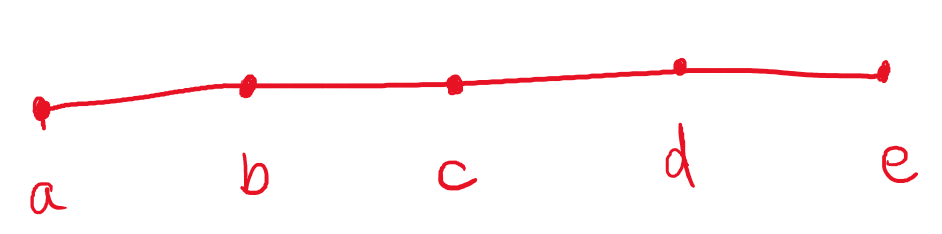
\includegraphics[scale=0.2]{./fig/ex-1.png}
\end{figure}
\[B_4(a)=\{a,b,c,d\} \subset B_3(c)=\{a,b,c,d,e\}\]
证明:若$B_7(a) \subset B_3(b)$则$B_7(a)=B_3(b)$。\\
\textbf{Proof:}
\[\forall x \in B_3(b) \ , \ d(x,a) \leq d(x,b)+d(b,a)<3+3=6<7 \ \Rightarrow \ x \in B_7(a)\]
\textbf{Q.E.D.}

\paragraph*{7.}$(X,d)$是距离空间,$A \subset X$,令$f(x)=\mathop \text{inf}\limits_{y \in A}d(x,y)$,证明$f(x)$连续。\\
\textbf{Proof:}
\[\forall x_1,x_2 \in X \ , \ y \in A \ , \ d(x_1,x_2) \leq d(x_1,y)+d(y,x_2)\]
取下极限
\[f(x_1) \leq d(x_1,x_2)+f(x_2) \ \Leftrightarrow \ f(x_1)-f(x_2) \leq d(x_1,x_2)\]
同理
\[f(x_2)-f(x_1) \leq d(x_1,x_2)\]
\[\Rightarrow \ |f(x_1)-f(x_2)| \leq d(x_1,x_2) \to 0\]
\[\forall \varepsilon>0 \ , \ d(x_1,x_2)<\delta=\varepsilon \quad \text{s.t.} \quad |f(x_1)-f(x_2)|<\varepsilon\]
\textbf{Q.E.D.}

\paragraph*{8.}证明$C^1[0,1]$是完备距离空间。\\
\textbf{Proof:}设$\{x_n(t)\}$是$C^1[0,1]$中的柯西列。
\[d(x_n(t),x_m(t))=\mathop \text{sup}\limits_{t \in [0,1]}|x_n(t)-x_m(t)|+\mathop \text{sup}\limits_{t \in [0,1]}|x_n'(t)-x_m'(t)|\]
由$C[0,1]$的完备性可知,我们只需要证明$\{x_n'(t)\}$是$C[0,1]$中的柯西列,即$x_n'(t) \rightrightarrows h(t) \in C[0,1]$。只需证
\[x_n(t) \rightrightarrows x(0)+\int_0^th(s)\dd s \qquad x(0)=\lim_{n \to \infty}x_n(0)\]
验证:
\[\left|x_n(t)-x(0)-\int_0^th(s)\dd s\right| \leq \left|x_n(0)+\int_0^tx_n'(s)\dd s-x(0)-\int_0^th(s)\dd s\right| \quad \text{微积分基本定理}\]
\[\leq \left|x_n(0)-x(0)\right|+\int_0^t|x_n'(s)-h(s)|\dd s \leq \left|x_n(0)-x(0)\right|+\mathop \text{sup}\limits_{t \in [0,1]}|x_n'(t)-h(t)| \to 0 \quad (n \to \infty)\]
且上述极限的取值与$t \in [0,1]$无关,故为一致收敛,原命题得证。\\
\textbf{Q.E.D.}

\paragraph*{8.}证明:闭球套定理成立的距离空间是完备距离空间。\\
\textbf{Proof:}原命题等价于设$(X,d)$中任一套闭球套$(r_n \to 0)$都有非空交,那么$(X,d)$完备。\\
设$\{x_n\}$是$X$中的柯西列,由它构造闭球套:
\[\forall k \in \mathbb{Z}_+ \ , \ \exists \, n_k>0 \quad \text{s.t.} \quad m,n \geq n_k \ , \ d(x_m,x_n)<\frac{1}{2^k} \ \Rightarrow \ x_n \in B_{\frac{1}{2^{k+1}}}(x_{n_k})\]
\[\Rightarrow \ \exists \, \{x_{n_k}\} \ (k=1,2,\cdots) \quad \text{s.t.} \quad \bar{B}_{\frac{1}{2^{k+1}}}(x_{n_{k+1}}) \subset \bar{B}_{\frac{1}{2^k}}(x_{n_k})\]
\[\text{由题设} \exists \,! \, x \in \bigcap_{k=1}^{\infty}\bar{B}_{\frac{1}{2^k}}(x_{n_k}) \ , \ d(x_{n_k},x) \to 0 \ (n \to \infty) \ \Rightarrow \ d(x_n,x) \to 0 \ (n \to \infty)\]
(柯西列+收敛子列$\ \Rightarrow \ $柯西列收敛)\\
\textbf{Q.E.D.}

\paragraph*{9.}设$(X,d)$完备,$\tilde{f}$为$X$上的一族连续函数,满足
\[\tilde{f}=\{F(x)|\forall x \in X \ , \exists \, M_x>0 \quad \text{s.t.} \quad |F(x)| \leq M_x\}\]

证明:$\exists \, M>0 \ , \ \exists \, U\text{(开集)} \in X \quad \text{s.t.} \quad \forall x \in U \ , \ F \in \tilde{f} \ , \ |F(x)| \leq M$\\
Proof($Baire$定理应用):设$E_n=\{x|x \in X \ , \ |F(x)| \leq n \ , \ F \in \tilde{f}\}$
\[\text{由题设} \forall x \in X \ , \ x \in E_{[M_x]+1} \ \Rightarrow \ X \subset \bigcup_{n=1}^{\infty}E_n \ \left(or \ X=\bigcup_{n=1}^{\infty}E_n \right)\]
$(X,d)$完备,由$Baire$定理,至少存在一个$M$使得$E_M$不是疏集,即存在一个开集$U \subset \bar{E}_M$
\[\forall x \in U \ , \ \exists \, \{x_n\} \subset E_M \ , \ x_n \to x \ (n \to \infty)\]
由连续性可知
\[|F(x)|=\lim_{n \to \infty}|F(x_n)| \leq M \ , \ \forall F \in \tilde{f}\]
\textbf{Q.E.D.}

\paragraph*{10.}在距离空间中证明:连续$\ \Leftrightarrow \ $开集的原像是开集。\\
Proof($\ \Rightarrow \ $):设$f:X \to Y$是连续映射,设$G \subset Y$是任一开集,要证$f^{-1}(G)$是$X$中的开集。
\[\forall x_0 \in f^{-1}(G) \ , \ f(x_0) \in G \ \Rightarrow \ \exists \, \varepsilon>0 \quad \text{s.t.} \quad B_{\varepsilon}(f(x_0)) \subset G\]
$f$是连续映射:
\[\exists \, \delta>0 \quad \text{s.t.} \quad d(y,x_0)<\delta \ , \ d_Y(f(y),f(x_0))<\varepsilon \ \Rightarrow \ f(B_{\delta}(x_0)) \subset B_{\varepsilon}(f(x_0)) \subset G\]
\[\Rightarrow \ B_{\delta}(x_0) \subset f^{-1}(G) \ \Leftrightarrow \ x_0\text{是}f^{-1}(G)\text{的内点,由}x_0\text{的任意性可得}f^{-1}(G)\text{是开集}\]
\begin{figure}[htbp]
    \center
    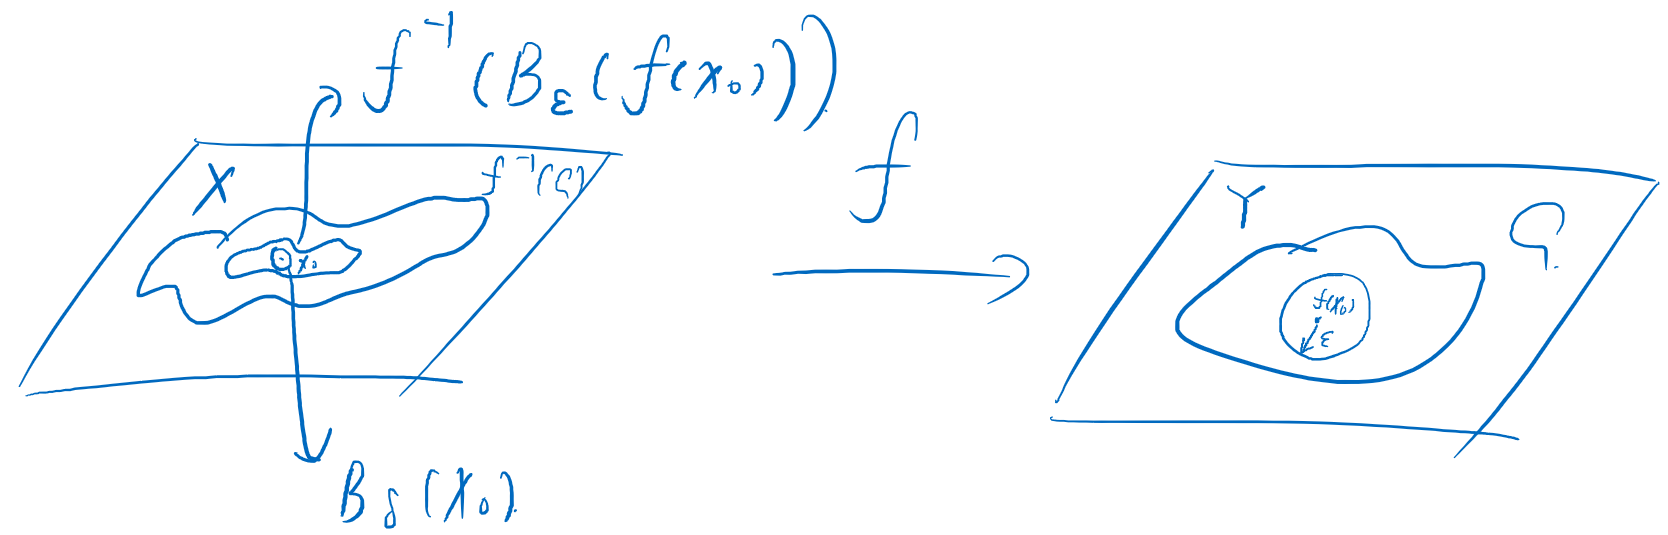
\includegraphics[scale=0.2]{./fig/ex-2.png}
\end{figure}
Proof($\ \Leftarrow \ $):设$f:X \to Y$满足开集的原像是开集,则$\forall x_0 \in X \ , \ \exists \, \varepsilon>0 \ , \ B_{\varepsilon}(f(x_0))$是$Y$中的开集。
\[\Rightarrow \ f^{-1}(B_{\varepsilon}(f(x_0)))\text{是$X$中的开集}, \ x_0 \in f^{-1}(B_{\varepsilon}(f(x_0)))\text{是内点}\]
\[\exists \, \delta>0 \ , \ f(B_{\delta}(x_0)) \subset B_{\varepsilon}(f(x_0)) \ \Rightarrow \ f\text{在}x_0\text{连续}\]
由$x_0$任意性可得$f$在$X$上连续。
\begin{figure}[htbp]
    \center
    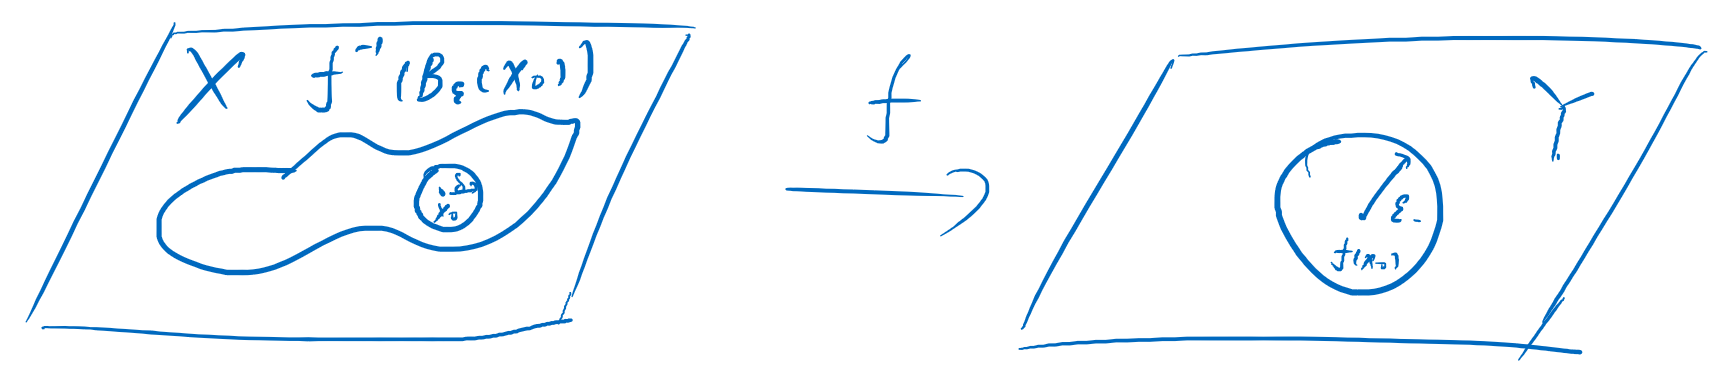
\includegraphics[scale=0.2]{./fig/ex-3.png}
\end{figure}
\textbf{Q.E.D.}

\paragraph*{11.}举例说明在压缩映射中(1)完备性不可少; \ (2)$d(Tx,Ty)<d(x,y) \ \forall x \neq y$是不充分的。
\[(1) \quad R-\{0\} \to R-\{0\} \quad x \mapsto \frac{1}{2}x \ \text{无不动点。}\]
\[(2) \quad T:[0,+\infty) \to [0,+\infty) \quad T(x)=x+\frac{1}{1+x}\]
Claim (2):
\[d(T(x),T(y))=\left|x+\frac{1}{1+x}-y-\frac{1}{1+y}\right|=\left|x-y-\frac{x-y}{(1+x)(1+y)}\right|\]
\[=\left|1-\frac{1}{(1+x)(1+y)}\right|d(x,y)<d(x,y)\]
\[T(x)=x \ \Rightarrow \ \frac{1}{1+x}=0 \ \Rightarrow \ x\text{无解,无不动点}\]
\textbf{Q.E.D.}

\paragraph*{12.}$T:X \to X \ , \ X$完备,$T$在闭球$\bar{B}_r(x_0) \ x_0 \in X$上为压缩映射,即满足
\[d(Tx,Ty) \leq \theta d(x,y) \ (\theta \in (0,1))\text{,且}d(x_0,Tx_0)<(1-\theta)r\]
证明:$T$在$\bar{B}_r(x_0)$上有唯一不动点。\\
\textbf{Proof:}只需证$T(\bar{B}_r(x_0)) \subset \bar{B}_r(x_0)$ (后续由完备闭子空间也是完备的可证)
\[\forall x \in \bar{B}_r(x_0) \ , \ d(Tx,x_0) \leq d(Tx,Tx_0)+d(Tx_0,x_0) \leq \theta d(x,x_0)+(1-\theta)r \leq \theta r+(1-\theta)r=r\]
\[\Rightarrow \ Tx \in \bar{B}_r(x_0) \ \text{由}x\text{的任意性} \ T(\bar{B}_r(x_0)) \subset \bar{B}_r(x_0)\]
把$T$限制在$\bar{B}_r(x_0)$上:$T:\bar{B}_r(x_0) \to \bar{B}_r(x_0) \ , \ T$为压缩映射,$\bar{B}_r(x_0)$是完备空间$X$上的闭子空间,所以$\bar{B}_r(x_0)$完备。由压缩映射定理即证。\\
\textbf{Q.E.D.}

\paragraph*{13.}$(t_0,s_0) \in \mathbb{R}^2 \ , \ f(t,s)$在$(t_0,s_0)$邻域$N$中连续,$s_0=f(t_0,s_0) \ , \ f_s(t,s)$在$N$中存在且在$(t_0,s_0)$连续,且$f_s(t_0,s_0)=0$。\\
证明:
\[\exists \, \delta>0 \ , \ x(t) \in C[t_0-\delta,t_0+\delta] \quad \text{s.t.} \quad x(t)=f(t,x(t)) \ , \ t \in [t_0-\delta,t_0+\delta] \ , \ x(t_0)=s_0 \ \text{有唯一解}\]
Solve:我们的思路是构造压缩映射$Tx=f(t,x(t))$来解决初值问题的证明:
\[d(Tx,Ty)=\mathop \text{sup}\limits_t|f(t,x)-f(t,y)|=\mathop \text{sup}\limits_t|f_x(t,\xi(t))||x-y| \leq \mathop \text{sup}\limits_t|f_x(t,\xi(t))|d(x,y)\]
\textbf{Proof:}
\[f_s(t,s) \in C(N) \ , \ f(t_0,s_0)=0 \ \Rightarrow \ \exists \, \delta>0 \quad \text{s.t.} \quad |t-t_0|,|s-s_0| \leq \delta \ , \ |f_s(t,s)|=\theta < 1\]
令
\[X=\{x(t) \in C[t_0-\delta,t_0+\delta] \ , \ x(t_0)=s_0 \ , \ \mathop \text{sup}\limits_{t \in [t_0-\delta,t_0+\delta]}|x(t)-s_0| \leq \frac{\delta}{2}\}\]
(极限不保严格不等号,所以上式最后一项取闭保持闭性)\\
\textbf{Claim} $X$是完备的\\
(\textbf{Proof:}$C[t_0-\delta,t_0+\delta]$是完备的,所以有
\[\forall \{x_n(t)\} \subset C[t_0-\delta,t_0+\delta] \ , \ \exists \, X_{\infty}(t) \quad \text{s.t.} \quad x_n(t) \rightrightarrows x_{\infty}(t)\]
\[\Rightarrow \ x_{\infty}(t_0)=\lim_{n \to \infty}X_n(t_0)=\lim_{n \to \infty}s_0=s_0\]
故$X$完备。\\
\textbf{Q.E.D.})\\
定义$T:X \to X \ : \ T(x(t))=f(t,x(t))$,下面验证定义良好(满足初值条件以及像在原空间中):
\[\text{1、} \ T(x(t_0))=f(t_0,x(t_0))=f(t_0,s_0)=s_0=x(t_0)\]
\[\text{2、} \ \mathop \text{sup}\limits_{t \in [t_0-\delta,t_0+\delta]}|T(x(t))-s_0|=\mathop \text{sup}\limits_{t \in [t_0-\delta,t_0+\delta]}|f(t,x(t))-s_0|=\mathop \text{sup}\limits_{t \in [t_0-\delta,t_0+\delta]}|f_s(t,\xi(t))||x-s_0| \leq \frac{\delta}{2}\]
\[\Rightarrow \ T(x(t)) \in X\]
\[d(Tx,Ty)=\mathop \text{sup}\limits_{t \in [t_0-\delta,t_0+\delta]}|f(t,x(t))-f(t,y(t))|=\mathop \text{sup}\limits_{t \in [t_0-\delta,t_0+\delta]}|f_s(t,\xi(t))||x(t)-y(t)| \leq \theta d(x,y)\]
$T$是压缩映射
\[\exists \, ! \, x(t) \in X \quad \text{s.t.} \quad x(t)=f(t,x(t))\]
\textbf{Q.E.D.}

\paragraph*{14.}证明:全有界集$A$的有限$\varepsilon$-网可取为$A$的子集。\\
这题主要用到了以下事实:
\[d(x,y)<r \ \Leftrightarrow \ x \in B_r(y) \ \Rightarrow \ B_r(y) \subset B_{2r}(x)\]
\begin{figure}[htbp]
    \center
    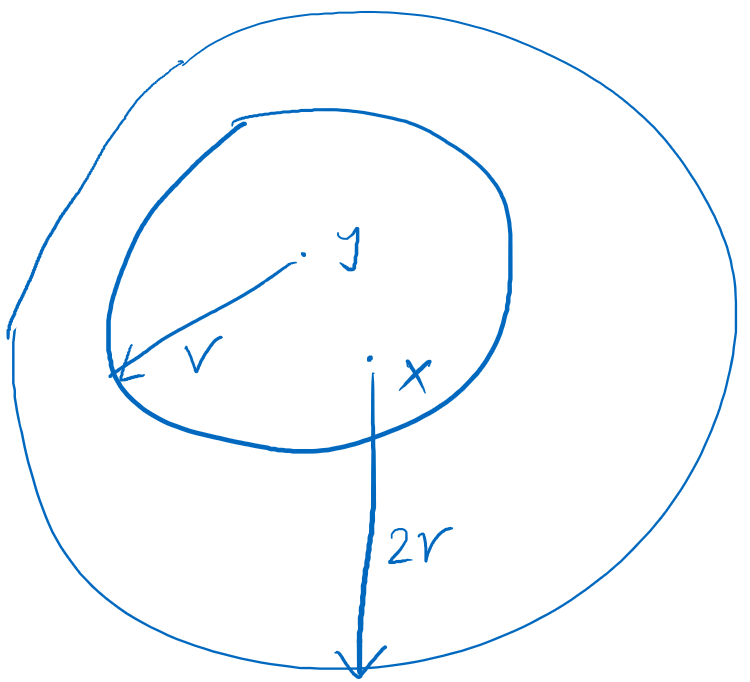
\includegraphics[scale=0.2]{./fig/ex-4.png}
\end{figure}
\textbf{Proof:}
\[\forall \varepsilon>0 \ , \ \exists \, A\text{有限}\frac{\varepsilon}{2}\text{-网} \ , \ N=\{x_1,x_2,\cdots,x_k\} \ , \ \text{若}B_{\frac{\varepsilon}{2}}(x_i) \cap A =\varnothing \ , \ \text{则可以把$x_i$从$N$中去掉}\]
\[\text{不妨设对每个} \ x_i \in N \ , \ B_{\frac{\varepsilon}{2}}(x_i) \cap A \neq \varnothing \ , \ \text{取} \ y_i \in B_{\frac{\varepsilon}{2}}(x_i) \cap A \ \Rightarrow \ B_{\frac{\varepsilon}{2}}(x_i) \subset B_{\varepsilon}(y_i)\]
\[\Rightarrow \ \tilde{N}=\{y_1,y_2,\cdots,y_k\}\text{为$A$的有限$\varepsilon$-网且} \ \tilde{N} \subset A\]
\textbf{Q.E.D.}

\paragraph*{15.}证明:$ \ C^1[0,1]$中的有界集$A$是$C[0,1]$中的相对紧集。
\begin{definition}[相对紧集]
    若集合$M$的闭包$\bar{M}$在空间中是紧集,则称$M$是相对紧集。
\end{definition}
$C[0,1]$是距离空间,故$C[0,1]$中的紧集是列紧的闭集,$\bar{A}$是闭集,故只需证明$\bar{A}$是列紧的。显然接下来我们是要利用$Arzela$定理分三步证明:

1、$A$在距离空间$C[0,1]$中有界(即一致有界); \ 2、$A$等度连续 ;\\
由1、2以及$Arzela$定理可以证明$A$是列紧的;

3、证明列紧集的闭包还是列紧的。\\
\textbf{Proof:}\\
\textbf{1.}
\[A\text{在}C^1[0,1]\text{中有界} \ \Rightarrow \ \exists \, K>0 \ , \ \forall x(t) \in A \quad \text{s.t.} \quad d_{C^1}(x(t),0) \leq K\]
\[\Rightarrow \ d_C(x(t),0) \leq d_{C^1}(x(t),0) \leq K \ \Rightarrow \ \text{$A$在距离空间$C[0,1]$中有界}\]
\textbf{2.}
\[\forall \varepsilon>0 \ , \ x(t) \in A \ , \ \exists \, t_1,t_2 \in [0,1] \quad \text{s.t.} \quad |x(t_1)-x(t_2)|=|x'(\xi)||t_1-t_2| \leq K|t_1-t_2|\]
\[\text{取} \ |t_1-t_2|<\frac{\varepsilon}{K} \ \Rightarrow \ |x(t_1)-x(t_2)|<\varepsilon\]
由1、2以及$Arzela$定理可得,$A$是列紧的;
\textbf{3.}
\[\text{任取}\{x_n(t)\}_{n=1}^{\infty} \subset \bar{A} \ \Rightarrow \ \forall x_n(t) \in \bar{A} \ , \ \exists \, y_n(t) \in A \quad \text{s.t.} \quad d_C(x_n(t),y_n(t))<\frac{1}{n}\]
因为$A$是列紧的:
\[\exists \, n_k \quad \text{s.t.} \quad y_{n_k}(t) \to y(t) \ (k \to \infty)\]
\[d_C(x_{n_k}(t),y(t)) \leq d_C(x_{n_k}(t),y_{n_k}(t))+d_C(y_{n_k}(t),y_{n_k}(t))\]
\[\leq \frac{1}{n_k}+d_C(y_{n_k}(t),y_{n_k}(t)) \to 0 \ (k \to \infty) \ \Rightarrow \ \bar{A}\text{列紧}\]
\textbf{Q.E.D.}

\paragraph*{16.}$X$是紧距离空间,$T:X \to X$是连续映射,满足$d(Tx,Ty)<d(x,y) \ \forall x \neq y$。\\
证明:$T$存在唯一不动点。

需要注意的是这里$T$不是一定压缩映射:\\
\textbf{例}
\[X=[0,1] \qquad Tx=\frac{x}{1+x}\]
\[|Tx-Ty|=\left|\frac{x}{1+x}-\frac{y}{1+y}\right|=\frac{|x-y|}{|1+x||1+y|}<|x-y| \quad (\forall x \neq y \in [0,1])\]
$T$有唯一不动点$T0=0$\\
\textbf{Proof:} 定义$f(x)=d(x,Tx)$,容易证明,$f$在$X$上连续,故由于$X$是紧集可知$f$有最小值,设$x_0$是$f$的极小值点。
\[\text{if} \ f(x_0)>0 \ \text{then} \ f(x_0) \leq d(Tx_0,T^2X_0)<d(x_0,Tx_0)=f(x_0)\]
矛盾,故$f(x_0)=0 \ \Rightarrow \ Tx_0=x_0$是不动点。\\
若$\exists \, y_0 \quad \text{s.t.} \quad Ty_0=y_0$,若$y_0 \neq x_0$,则
\[0<d(x_0,y_0)=d(Tx_0,Ty_0)<d(x_0,y_0)\]
矛盾,所有$y_0=x_0$,不动点唯一。\\
\textbf{Q.E.D.}

\paragraph*{17.}证明$Banach$空间$c_0$可分。
\[c_0=\{x=\{\xi_k\}_{k=1}^{\infty}|\lim_{k \to \infty}\xi_k=0\} \qquad ||x||=\mathop \text{sup}\limits_{k}|\xi_k|\]
\textbf{Proof:}\\
\[\text{由} \ \lim_{k \to \infty}\xi_k=0 \ \text{可知,我们可以构造下列序列组成$c_0$的子集} \ c_0'=\{x'=(\xi_i,\xi_2,\cdots,\xi_k,0,0,\cdots)\}\]
令$A=\{r=\{r_k\}_{k=1}^{\infty}|r_k \in \mathbb{Q} \ , \ \exists \, n>0 \ , \ \forall j>n \ , \ r_j=0\}$
\[\forall \varepsilon>0 \ , \ x=\{\xi_k\}_{k=1}^{\infty} \in c_0 \ , \ \lim_{k \to \infty}\xi_k=0 \ \Rightarrow \ \exists \, N>0 \ , \ \forall n \geq N \quad \text{s.t.} \quad |\xi_n|<\varepsilon\]
\[\exists \, r=(r_1,r_2,\cdots,r_N,0,0,\cdots) \in A \quad \text{s.t.} \quad ||x-r||=\mathop \text{sup}\limits_{k \in \mathbb{N}_+}|r_k-\xi_k| \leq \text{max}\left\{\mathop \text{sup}\limits_{k \in \mathbb{N}_+}|r_k-\xi_k| \ , \ \varepsilon\right\}<\varepsilon\]
因为
\[A=\bigcup_{k=1}^N\mathbb{Q} \qquad \text{card}(c_0')=\text{card}(A)=\text{card}(\mathbb{Q})\]
故$c_0$是可分的。\\
\textbf{Q.E.D.}

\paragraph*{18.}证明离散形式的$H\ddot{o}lder$不等式
\[\sum_{i=1}^n|x_iy_i| \leq \left(\sum_{i=1}^n|x_i|^p\right)^{\frac{1}{p}}\left(\sum_{i=1}^n|y_i|^q\right)^{\frac{1}{q}} \quad (p,q>0 \ , \ \frac{1}{p}+\frac{1}{q}=1 \ , \ x_i,y_i \in \mathbb{R} \ \text{or} \ \mathbb{C})\]
和$Minkowski$不等式
\[\left(\sum_{i=1}^n|x_i+y_i|^p\right)^{\frac{1}{p}} \leq \left(\sum_{i=1}^n|x_i|^p\right)^{\frac{1}{p}}+\left(\sum_{i=1}^n|y_i|^p\right)^{\frac{1}{p}} \quad (p \geq 1 \ , \ x_i,y_i \in \mathbb{R} \ \text{or} \ \mathbb{C})\]
Proof($H\ddot{o}lder$不等式):设
\[A=\left(\sum_{i=1}^n|x_i|^p\right)^{\frac{1}{p}} \qquad B=\left(\sum_{i=1}^n|y_i|^q\right)^{\frac{1}{q}}\]
由$Young$不等式:
\[\frac{|x_i| \cdot |y_i|}{A \cdot B} \leq \frac{1}{p}\frac{|x_i|^p}{A^p}+\frac{1}{q}\frac{|y_i|^q}{B^q} \ \Rightarrow \ \frac{1}{A \cdot B}\sum_{i=1}^n|x_iy_i| \leq \frac{1}{pA^p}\sum_{i=1}^n|x_i|^p+\frac{1}{qB^q}\sum_{i=1}^n|y_i|^q=1\]
\[\Rightarrow \ \sum_{i=1}^n|x_iy_i| \leq A \cdot B=\left(\sum_{i=1}^n|x_i|^p\right)^{\frac{1}{p}} \cdot \left(\sum_{i=1}^n|y_i|^q\right)^{\frac{1}{q}}\]
\textbf{Q.E.D.}\\
Proof($Minkowski$不等式):
\[\sum_{i=1}^n|x_i+y_i|^p=\sum_{i=1}^n|x_i+y_i||x_i+y_i|^{p-1} \leq \sum_{i=1}^n|x_i||x_i+y_i|^{p-1}+\sum_{i=1}^n|y_i||x_i+y_i|^{p-1}\]
\[\leq \left(\sum_{i=1}^n|x_i|^p\right)^{\frac{1}{p}}\left(\sum_{i=1}^n|x_i+y_i|^{q(p-1)}\right)^{\frac{1}{q}}+\left(\sum_{i=1}^n|y_i|^p\right)^{\frac{1}{p}}\left(\sum_{i=1}^n|x_i+y_i|^{q(p-1)}\right)^{\frac{1}{q}}\]
\[\frac{1}{p}+\frac{1}{q}=1 \ \Leftrightarrow \ p=(p-1)q\]
\[\leq \left(\sum_{i=1}^n|x_i|^p\right)^{\frac{1}{p}}\left(\sum_{i=1}^n|x_i+y_i|^{p}\right)^{1-\frac{1}{p}}+\left(\sum_{i=1}^n|y_i|^p\right)^{\frac{1}{p}}\left(\sum_{i=1}^n|x_i+y_i|^{p}\right)^{1-\frac{1}{p}}\]
\[\Rightarrow \ \left(\sum_{i=1}^n|x_i+y_i|^p\right) \cdot \left(\sum_{i=1}^n|x_i+y_i|^{p}\right)^{\frac{1}{p}-1} \leq \left(\sum_{i=1}^n|x_i|^p\right)^{\frac{1}{p}}+\left(\sum_{i=1}^n|y_i|^p\right)^{\frac{1}{p}}\]
\[\Leftrightarrow \ \left(\sum_{i=1}^n|x_i+y_i|^{p}\right)^{\frac{1}{p}} \leq \left(\sum_{i=1}^n|x_i|^p\right)^{\frac{1}{p}}+\left(\sum_{i=1}^n|y_i|^p\right)^{\frac{1}{p}}\]
\textbf{Q.E.D.}

\paragraph*{19.}设$m(E)<+\infty \ , \ f \in L^{\infty}(E)$,证明:
\[\lim_{p \to \infty}||f||_{L^p}=||f||_{L^{\infty}}\]
\textbf{Proof:}
\[||f||_{L^p(E)}=\left(\int_E|f|^p\dd t\right)^{\frac{1}{p}}=\left(\int_{E/E_0}|f|^p\dd t\right)^{\frac{1}{p}} \leq \left(m(E) \cdot ||f||^p_{L^{\infty}(E)}\right)^{\frac{1}{p}}=m(E)^{\frac{1}{p}}||f||^p_{L^{\infty}(E)}\]
\[\lim_{p \to \infty}||f||_{L^p(E)} \leq \lim_{p \to \infty}m(E)^{\frac{1}{p}}||f||^p_{L^{\infty}(E)}=||f||^p_{L^{\infty}(E)}\]
另一方面,我们令$\forall \varepsilon>0 \ , \ m(|f| \geq M-\varepsilon)=\delta>0 \ \text{where} \ M:=||f||_{L^{\infty}(E)}$
\[||f||_{L^p(E)}=\left(\int_E|f|^p\dd t\right)^{\frac{1}{p}}=\left(\int_{f \geq M-\varepsilon}|f|^p\dd t+\int_{f<M-\varepsilon}|f|^p\dd t\right)^{\frac{1}{p}}\]
\[\geq \left(\int_{|f| \geq M-\varepsilon}|M-\varepsilon|^p\dd t+\int_{|f|<M-\varepsilon}|f|^p\dd t\right)^{\frac{1}{p}} \geq |M_\varepsilon|\delta^{\frac{1}{p}}\]
由$\varepsilon$的任意性:
\[\lim_{p \to \infty}||f||_{L^p(E)} \geq \lim_{p \to \infty} |M_\varepsilon|\delta^{\frac{1}{p}}=||f||_{L^{\infty}(E)}\]
综上所述,有
\[\lim_{p \to \infty}||f||_{L^p}=||f||_{L^{\infty}}\]
\textbf{Q.E.D.}
\end{document}
